\chapter{Simulação}
\label{chap:simulation}
Nessa seção, busca-se validar a abordagem integrada de Modelagem por meio de Redes de Petri Coloridas (RPC) e Controle Cooperativo. Para realizar essa validação, optou-se por empregar a estratégia de simulação, utilizando um sistema multiagente composto por diversos componentes, os quais foram concebidos para representar um ambiente similar a um sistema industrial.

Neste processo de simulação, são utilizadas ferramentas de software dedicadas à modelagem em RPC, com destaque para o CPN-Tools.\footnote{pode ser acessada em \texttt{https://cpntools.org/}} Essa ferramenta oferece funcionalidades específicas para a edição, simulação e análise de Redes de Petri Coloridas. A escolha do CPN-Tools visa proporcionar uma representação fiel e detalhada do sistema em estudo.

Para a implementação do algoritmo matemático de consenso, optou-se por utilizar a linguagem de programação Python. Essa escolha deve-se à reputação da linguagem como sendo de alto nível, funcional e orientada a objetos, oferecendo assim uma abordagem versátil e eficiente para a execução do algoritmo em questão.

Ao unir a simulação do sistema multiagente com as capacidades do CPN-Tools e a flexibilidade do Python, almeja-se obter resultados robustos que validem a eficácia da abordagem proposta. Esta seção detalhará o processo de simulação, desde a definição dos parâmetros até a análise crítica dos resultados obtidos, proporcionando uma compreensão clara e abrangente da validade e desempenho da abordagem integrada.

No método integrado de modelagem e controle baseado em Redes de Petri Coloridas e sistemas multiagentes, propõe-se uma subdivisão de responsabilidade entre os sistemas envolvidos no processo. Esses sistemas são o sistema supervisório, o sistema de automação e o sistema de controle cooperativo. A organização desses sistemas é ilustrada na figura \ref{fig:topologia_integrada}, onde o sistema supervisório se comunica com o sistema de automação, e este, por sua vez, com o sistema de controle cooperativo.

\begin{figure}[ht]
\centering
\caption{Organização dos sistemas na Abordagem Integrada para sistemas multiagentes industriais.}
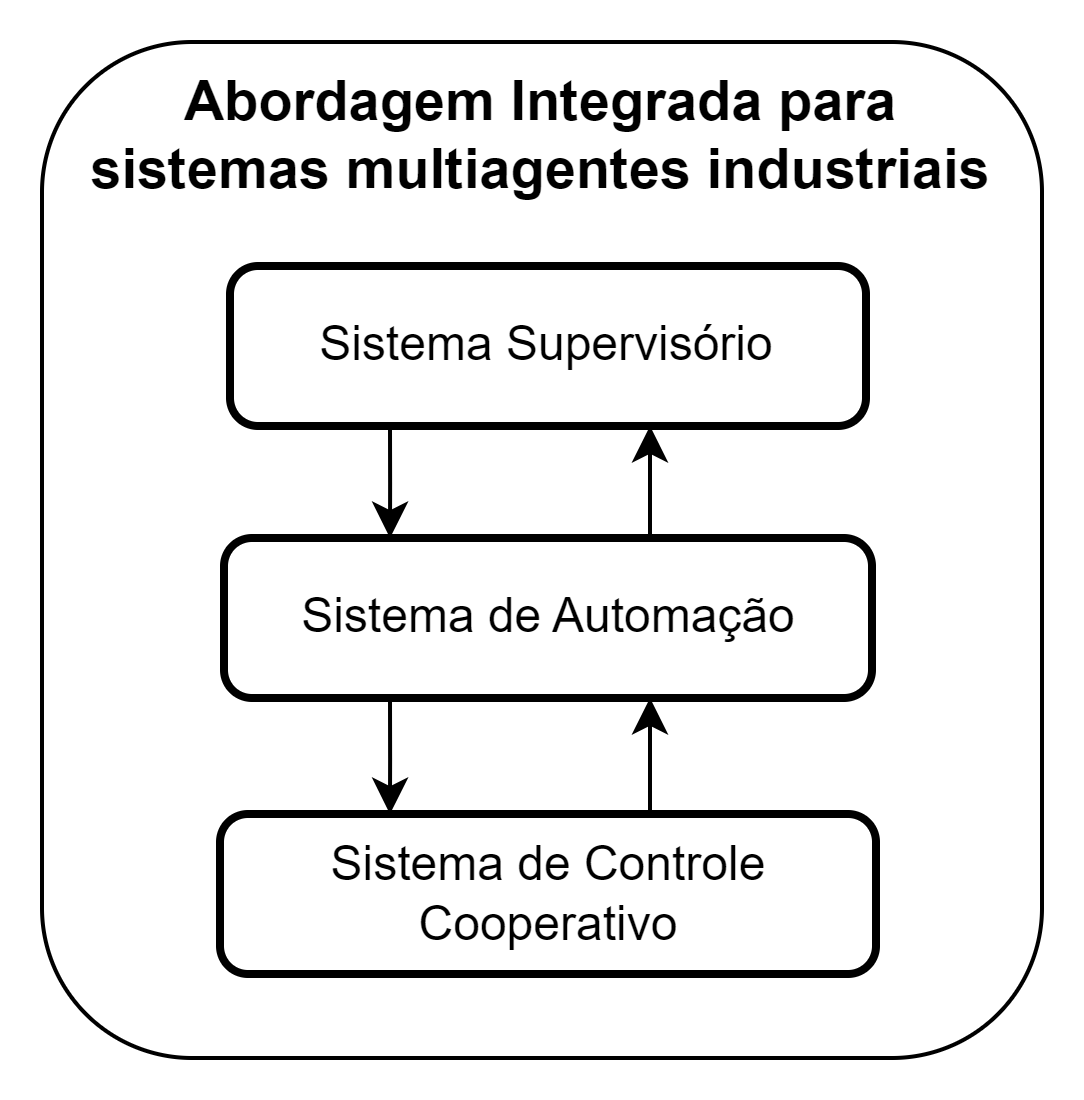
\includegraphics[width=0.5\linewidth]{figures/Simulation/Planta/topologia_integrada.png}
\label{fig:topologia_integrada}
\legend{Fonte: Elaborado pelo autor.}
\end{figure}

Na modelagem proposta, o sistema supervisório é encarregado dos requisitos e comandos para o sistema, como o controle dos horários, a ordem de chegada dos trens e outros parâmetros de alto nível. Abaixo, o sistema de automação é responsável por promover um protocolo para o segmento de trajetória e ultrapassagens, conforme ordenado pelo sistema supervisório. Este sistema de automação pode ser modelado utilizando as Redes de Petri Coloridas.

Por fim, abaixo do sistema de automação, temos o sistema de controle cooperativo, responsável por otimizar as referências de velocidade e trajetória dentro das restrições e protocolos estabelecidos pelo sistema de automação.







\section{Planta Industrial}
A gestão de vagões em uma planta industrial, que permite a ultrapassagem entre eles por meio de mudanças nas pistas, representa uma abordagem inovadora no contexto ferroviário industrial. Esse sistema dinâmico busca otimizar o movimento e a alocação de vagões, proporcionando flexibilidade e eficiência operacional.

A otimização da trajetória e da velocidade tornou-se uma prioridade devido à necessidade de reduzir o consumo de energia nos trens de carga para combater o efeito estufa. No estudo de \cite{train2023}, foi proposto um método de aprendizado por reforço para otimizar a velocidade de múltiplos agentes, visando alcançar eficiência energética, pontualidade e precisão no estacionamento. O autor examinou estudos de caso em Pequim, explorando abordagens como controle preditivo fuzzy, algoritmos genéticos e algoritmos de operação inteligente de trens.

O estudo conduzido por \cite{wang2017} propõe uma nova abordagem de otimização de trajetória para trens em linhas de via única, com foco na minimização de atrasos operacionais e na redução do consumo de energia. A metodologia desenvolvida tem como objetivo principal encontrar perfis de velocidade ótimos que permitam mitigar os atrasos e otimizar o uso de energia dos trens. Este método utiliza conjuntos de restrições de horários para trens em situações de atraso, os quais fornecem janelas de tempo e velocidade viáveis e eficientes ao longo das rotas. Além disso, a minimização do consumo de energia é considerada como uma função objetivo relevante. A aplicabilidade dessa abordagem é demonstrada por meio de estudos de caso envolvendo trens operando em um corredor ferroviário de via única na Holanda, considerando diferentes cenários de atraso inicial.

No contexto da planta apresentada, foram realizadas duas simulações distintas. A primeira envolveu apenas dois agentes, representados por autômatos, que colaboram no transporte e descarregamento de objetos. Nesse cenário mais simples, os agentes têm necessidades de ultrapassagem simples entre si, com um autômato responsável por mover objetos e cargas, e o outro encarregado de transportá-las. No segundo caso, foi modelada e controlada uma planta mais complexa, composta por um circuito dinâmico de trens. Estes apresentam restrições físicas de ultrapassagem e obedecem a protocolos determinados pelo controle supervisório, que emite comandos de ultrapassagem conforme as movimentações das junções de trilhos nas pistas.



\section{Caso de Simulação - Ultrapassagem Simples}
No primeiro cenário de simulação, foi delineado um sistema com uma única restrição: cada agente possui uma função específica e é essencial que cooperem para realizar o processo. Além disso, foi proposto um sistema de ultrapassagem simplificado, no qual não há restrições para ultrapassar, porém os agentes devem cooperar para executar a tarefa conjuntamente.
\subsection{Apresentação da planta}
No cenário de simulação simplificada, uma configuração composta por dois agentes é estabelecida, no qual um agente detém a responsabilidade específica pelo transporte, enquanto o outro é encarregado da manipulação da carga. Este arranjo é visualizado na Figura \ref{fig:simple_case}, onde ambos os agentes cooperam para efetuar o movimento de um objeto de uma coluna para outra, uma descrição de cada momento é dada no quadro \ref{quadro:sequencia_eventos}.

\begin{figure}[ht]
\centering
\caption{Ambiente com dois agentes: um responsável pela manipulação de objetos e o outro pelo transporte.}
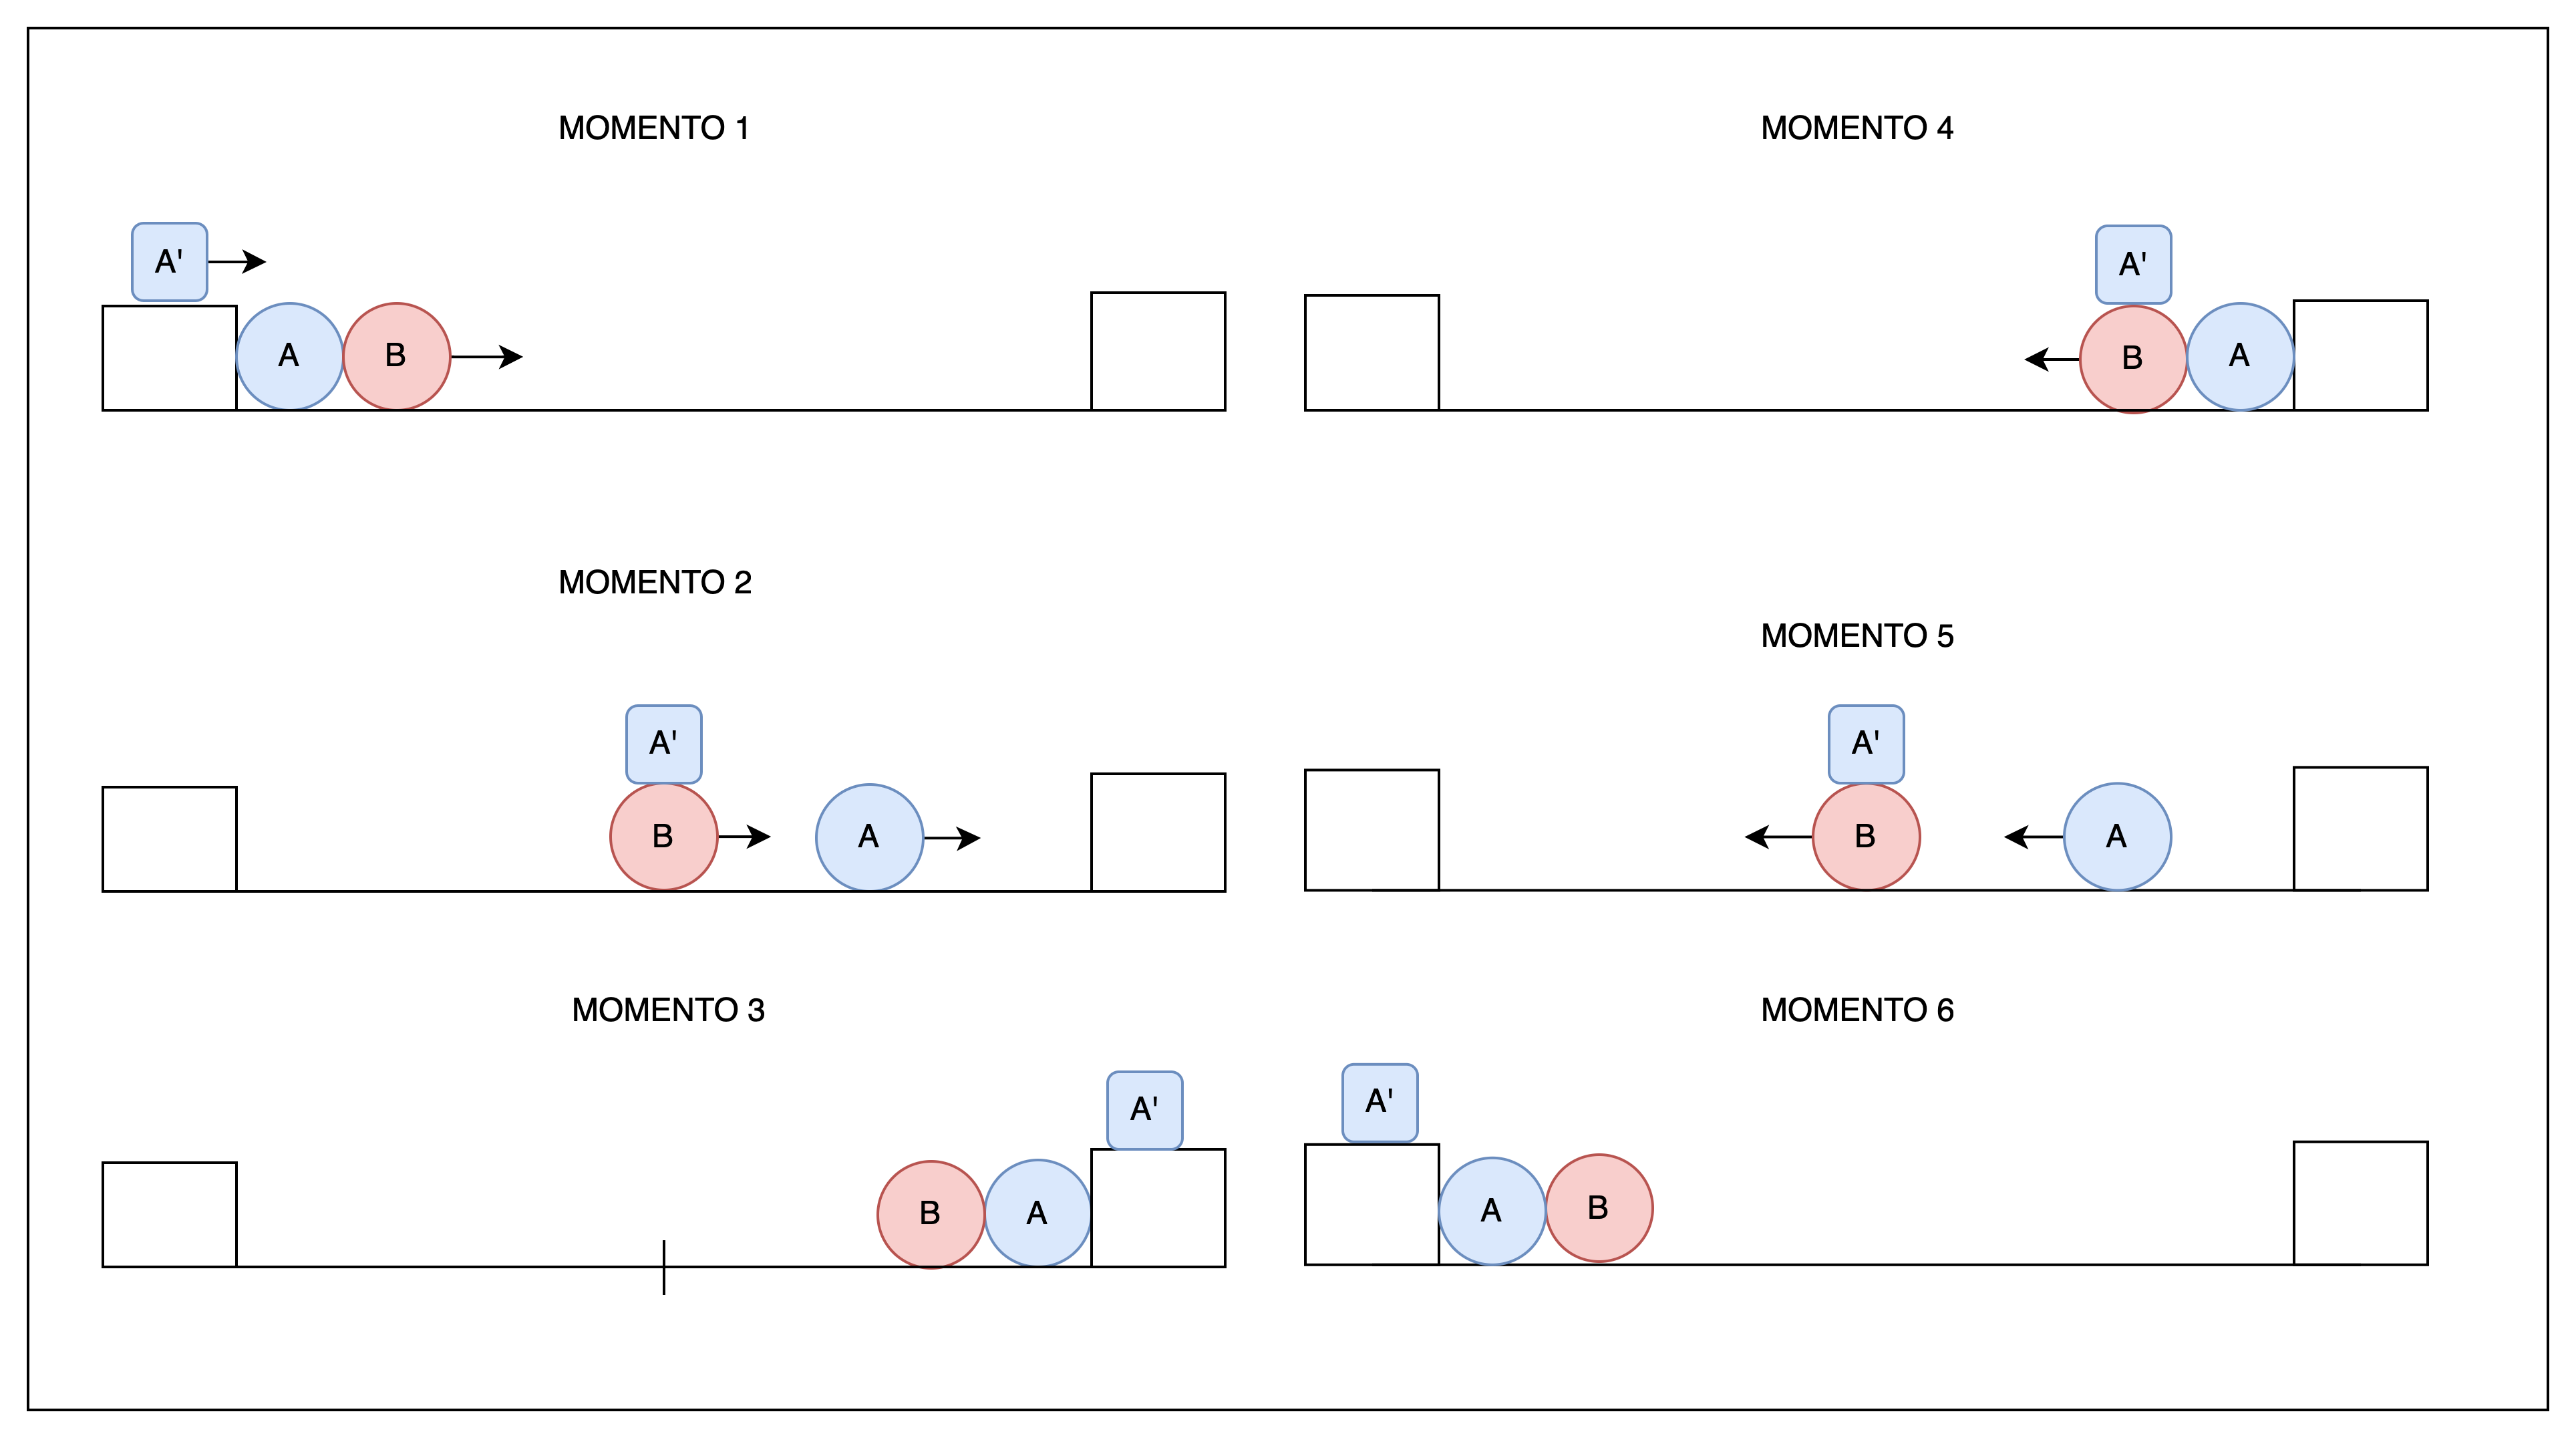
\includegraphics[width=1\linewidth]{figures/Simulation/Simples/caso_simples.png}
\label{fig:simple_case}
\legend{Fonte: Elaborado pelo autor.}
\end{figure}

\begin{quadro}[h]
\centering
\caption{Sequência de Eventos para Manipulação e Transporte de Objetos}
\begin{tabularx}{\textwidth}{|c|X|}
\hline
\textbf{Momento} & \textbf{Descrição} \\
\hline
1 & O manipulador A encontra-se na posição inicial com o transportador B, e A' encontra-se na coluna da esquerda. O manipulador A coloca o objeto em B para transporte e posteriormente sai em direção à segunda coluna. \\
\hline
2 & O manipulador ultrapassa o transportador em direção à segunda coluna. \\
\hline
3 & Os dois agentes chegam ao mesmo tempo na referência desejada e o manipulador retira o objeto A' do transportador e passa para a segunda coluna. \\
\hline
4 & O manipulador pega A' e põe no transportador. \\
\hline
5 & O manipulador sai atrasado em direção à primeira coluna. \\
\hline
6 & O manipulador e o transportador chegam na coluna à esquerda ao mesmo tempo, e o manipulador retira A' do transportador e põe na primeira coluna. \\
\hline
\end{tabularx}
\legend{Fonte: Elaborado pelo autor.}
\label{quadro:sequencia_eventos}
\end{quadro}

\subsection{Modelagem em redes de Petri}
Na modelagem em Rede de Petri Colorida, foram estabelecidos dois conjuntos de cores distintos. O primeiro conjunto, em cor vermelha, é designado para representar o recurso necessário à movimentação dos agentes, enquanto o segundo conjunto, em azul, simboliza o objeto A'. Na figura \ref{fig:simple_case_rpc}, é possível visualizar a representação em RPC, onde a porção superior da rede denota o protocolo de IDA (esquerda para direita), enquanto a parte inferior corresponde ao protocolo de Volta (direita para esquerda). Dentro do processo de IDA e VOLTA, houve uma subdivisão em lugares referentes ao Agente B (retângulo superior) e ao Agente A (retângulo inferior).
Na RPC, ainda na figura \ref{fig:simple_case_rpc} as transições T1 e T2 representam os momentos de sincronização e transferência de material entre agentes. Em T1, ocorre a ação em que o manipulador A remove o material da coluna e o coloca no transportador B, enquanto em T2, o manipulador realiza o movimento inverso, retirando o material do transportador. A porção inferior do grafo representa o mesmo processo de movimentação, porém de direita para esquerda, denotando o caminho de volta.    
\begin{figure}[ht]
\centering
\caption{Modelagem e rede de Petri Colorida para o caso com 2 agentes}
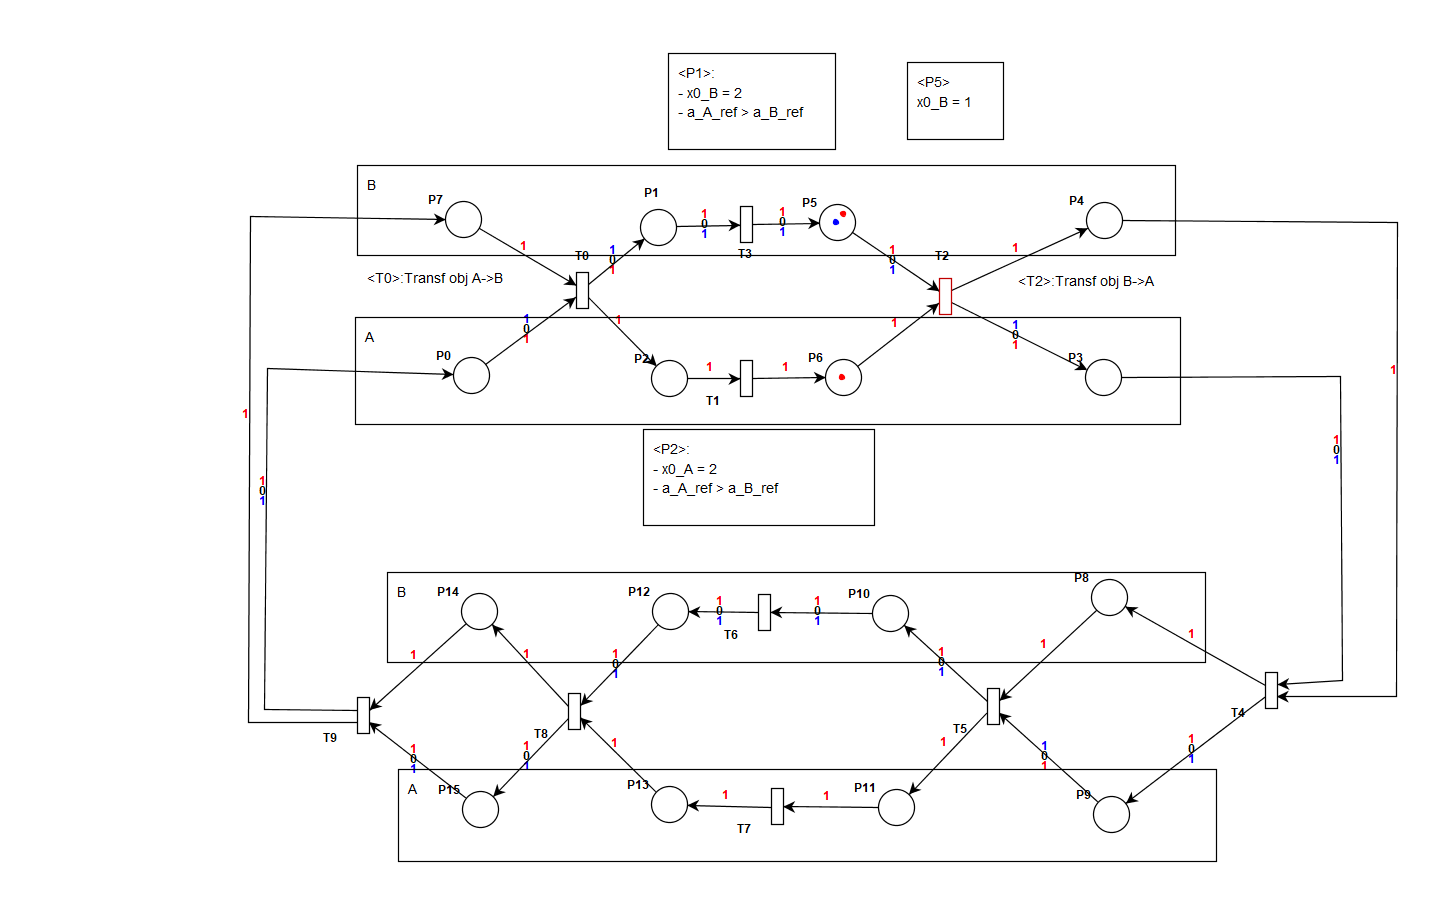
\includegraphics[width=1\linewidth]{figures/Simulation/Simples/simple_case_rpc.png}
\label{fig:simple_case_rpc}
\legend{Fonte: Elaborado pelo autor.}
\end{figure}

\subsection{Controle Cooperativo Aplicado}
No contexto da aplicação do controle cooperativo para dois agentes, é estabelecida a matriz de grafos, conforme representado na Figura \ref{fig:grafo_simple_case}. 

\begin{figure}[ht]
\centering
\caption{Grafo Multiagente para o caso com 2 agentes}
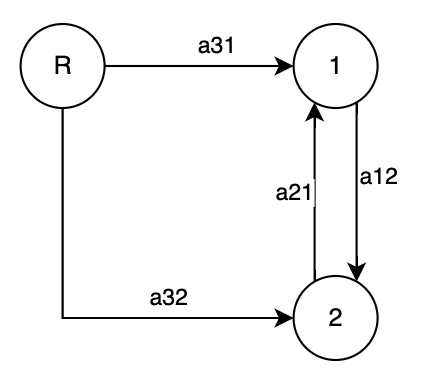
\includegraphics[width=0.3\linewidth]{figures/Simulation/Simples/grafo_simple_case.png}
\label{fig:grafo_simple_case}
\legend{Fonte: Elaborado pelo autor.}
\end{figure}

A primeira parte do algoritmo de controle cooperativo é definir os valores dos pesos entre agentes, onde o agente \( R \) é considerado como a referência. No problema proposto, foram definidos \( a_{31} = 0.5 \), \( a_{12} = 0.1 \), \( a_{21} = 0.1 \) e \( a_{32} = 0.3 \). Posteriormente, define-se a matriz de adjacência \( A \) e a matriz diagonal tal que \( A^T[0] \) corresponde à primeira linha de \( A \) transposta, \( A^T[1] \) à segunda linha e assim por diante, como demonstrado a seguir:
\[
A = \begin{bmatrix}
0 & a_{12} & 0 \\
a_{21} & 0 & 0 \\
a_{31} & a_{32} & 0
\end{bmatrix} ,
D = \begin{bmatrix}
sum(A^{T}[0]) & 0 & 0 \\
0 & sum(A^{T}[1]) & 0 \\
0 & 0 & sum(A^{T}[2])
\end{bmatrix}
\]
Para a construção da matriz Laplaciana, o valor final da matriz é determinado de acordo com a Equação \ref{eq:matriz_L1}, resultando no seguinte valor de L.
\[
L = \begin{bmatrix}
    sum(A^{T}[0]) & -a_{12} & 0 \\
    -a_{21} & sum(A^{T}[1]) & 0 \\
    -a_{31} & -a_{32} & sum(A^{T}[2])
    \end{bmatrix}
\]
Por fim o sistema resultante em espaço de estados é dado pelos seguintes valores de $A$, $B$, $C$ e $D$;
\[
A = -L 
 , 
 B = \begin{bmatrix}
    1\\
    0\\
    0\\
\end{bmatrix}
 ,
C = \begin{bmatrix}
    1 & 0 & 0\\
    0 & 1 & 0\\
    0 & 0 & 1\\
\end{bmatrix}
 ,
D = 0
\]
Na realização da simulação, foram estabelecidos dois cenários distintos. No primeiro cenário, ilustrado pelo gráfico de ultrapassagem na figura \ref{fig:simple_ultrapassagem}, ocorre uma situação na qual o Manipulador (Agente A) necessita ultrapassar o Transportador (Agente B) para atingir a referência, resultando em uma proximidade temporal notável na chegada dos dois agentes à posição desejada.
\begin{figure}[ht]
\centering
\caption{Comportamento do sistema em condição de ultrapassagem}
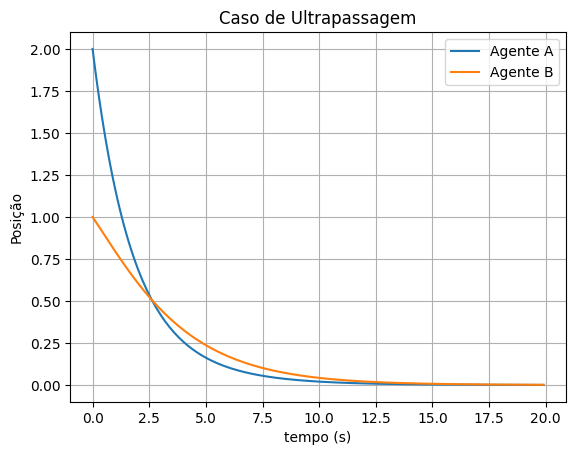
\includegraphics[width=0.8\linewidth]{figures/Simulation/Simples/simple_ultrapassagem.png}
\label{fig:simple_ultrapassagem}
\legend{Fonte: Elaborado pelo autor.}
\end{figure}

No segundo cenário, onde não ocorre ultrapassagem, foram atribuídos diferentes pesos entre os agentes e a referência. O agente com o maior peso (Agente A) apresenta um deslocamento mais rápido, enquanto o outro agente possui um movimento mais lento, o que simboliza o consenso para diferentes dinâmicas, conforme exemplificado na figura \ref{fig:simple_n_ultrapassagem}.

\begin{figure}[ht]
\centering
\caption{Comportamento do sistema em condição de não ultrapassagem}
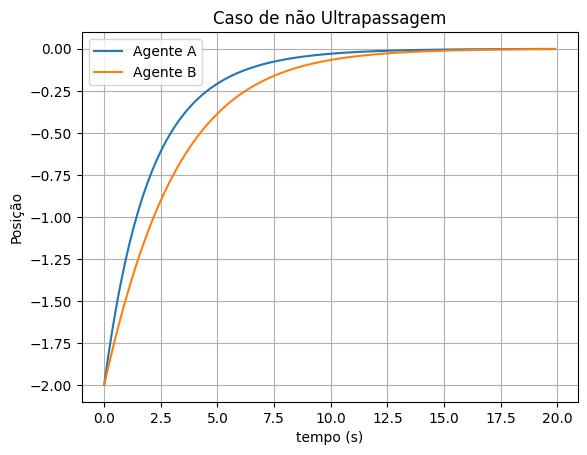
\includegraphics[width=0.8\linewidth]{figures/Simulation/Simples/simple_n_ultrapassagem.png}
\label{fig:simple_n_ultrapassagem}
\legend{Fonte: Elaborado pelo autor.}
\end{figure}


\section{Caso de simulação - Ultrapassem Complexa}
No contexto da simulação empregada nesse capítulo, ao incorporar a capacidade de ultrapassagem, a planta industrial adquire versatilidade, possibilitando a reorganização estratégica dos vagões para atender a demandas específicas. Essa funcionalidade torna-se particularmente valiosa em situações onde é necessário priorizar determinados vagões, reduzir tempos de espera ou melhorar o desempenho global do sistema ferroviário dentro do contexto da planta industrial.

A implementação de mudanças nas pistas como um meio de permitir a ultrapassagem requer uma coordenação precisa e um controle eficaz do sistema. Técnicas como Redes de Petri Coloridas (RPC) ou algoritmos de controle cooperativo podem ser empregados para modelar e simular o comportamento dinâmico da planta, considerando as interações entre os vagões e as mudanças nas pistas.

Um exemplo de representação desse sistema escolhido é demonstrada na figura \ref{fig:pista_com_dois_agentes}, tal que:
\begin{itemize}
    \item Os componentes $L_1$ e $L_2$ ilustrados em formato triangular são os vagões que representam os dois autômatos, ou agentes do sistema.
    \item As curvas $d_1,d_2,..,d_6$ representam as pistas pelas quais os vagões se locomovem, de modo os dois vagões estão posicionados incialmente na pista denominada de $d_1$.
    \item os elementos $x_1,x_2,x_3,x_4$ representam as quatro chaves responsáveis por fazer a mudança de via, elas podem comutar em duas posições diferentes a posição $b$ que representa o caminho de menor comprimento ou a posição $a$ que representa o caminho de maior comprimento.
\end{itemize}

\begin{figure}[h]
\centering
\caption{Planta com pista, vagões e pontos de mudança de via }
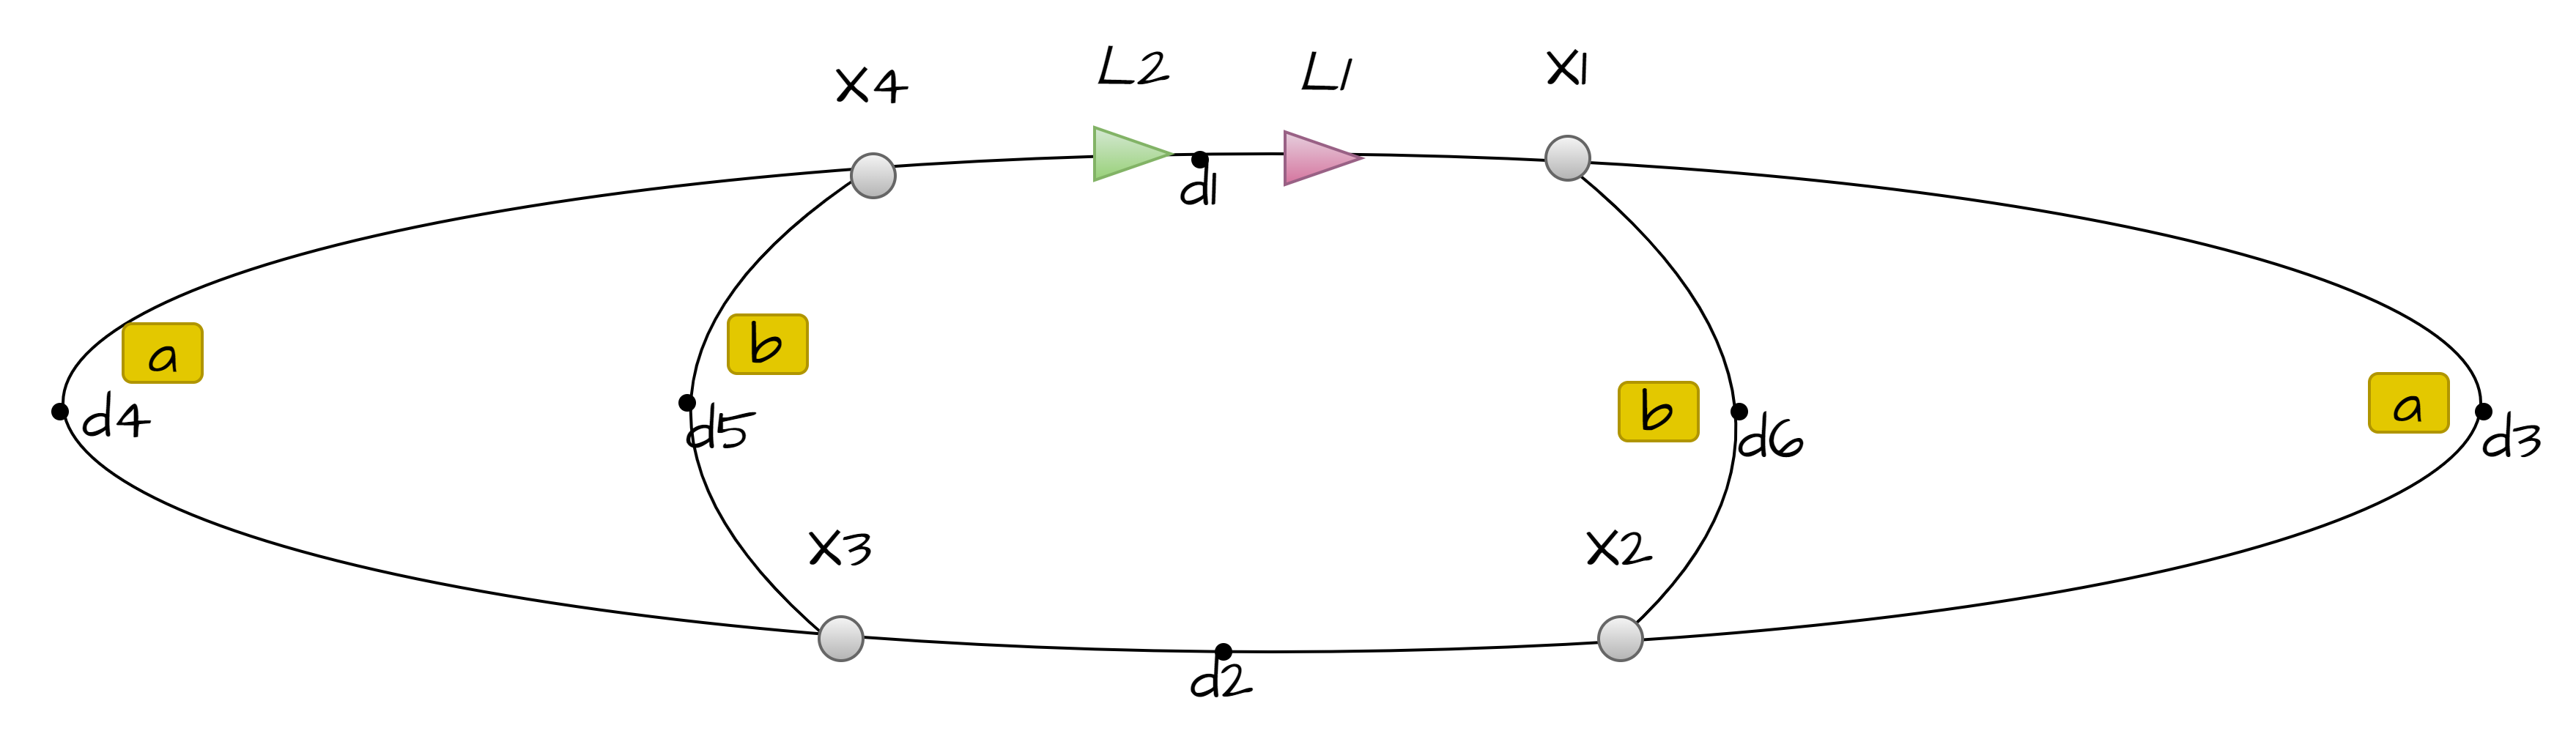
\includegraphics[width=1\linewidth]{figures/Simulation/Planta/planta_dois_agentes.png}
\label{fig:pista_com_dois_agentes}
\legend{Fonte: Elaborado pelo autor.}
\end{figure}

Para a simulação específica, os vagões movem-se entre pistas, e para efetuar uma ultrapassagem, é necessário que o vagão a ser ultrapassado siga pelo caminho mais longo, enquanto o vagão ultrapassante escolhe o caminho mais curto.

A chave de ultrapassagem foi designada como $x_1$. Quando o comando de ultrapassagem é acionado, inicialmente a chave se move para a posição $a$, assegurando o desvio para a pista mais longa. Em seguida, ela se move para a posição $b$, garantindo o desvio para a pista mais curta.

A chave $x_2$ desempenha o papel de primeiro desviar para a posição $b$, para receber o vagão da pista $d_6$. Posteriormente, comuta para a posição $a$, para receber o vagão da pista $d_3$.

As chaves $x_3$ e $x_4$ permanecem fixas na posição $b$, assegurando o percurso mais curto. Esse arranjo permite uma ultrapassagem de vagões de forma segura e otimizada entre as pistas.

\subsection{Modelagem em Redes de Petri Colorida}
\label{sec:model_RPC}
Para a modelagem do sistema proposto em Redes de Petri Colorida, foi definido o seguinte conjunto de cores para representar o tipo de token que vai ser alocado nos lugares da RPC de acordo com o seguinte quadro \ref{qua:conj_cores}.

\begin{quadro}[h]
\centering
\caption{Conjunto de Cores na RPC}
\begin{tabularx}{\textwidth}{|c|c|X|X|}
\hline
\textbf{Nomenclatura} & \textbf{Tipo}    & \textbf{Comando}                             & \textbf{Descrição} \\
\cline{1-4}
D & Inteiro & \texttt{colset D = int;} 
& Conjunto que indica a sequência dos vagões, onde o número 1 representa o vagão à frente, o número 2 representa o vagão atrás do 1, e assim por diante. \\ 
\cline{1-4}
X & String  & \texttt{colset X = string;} 
& Conjunto que representa a posição em que a chave se encontra, exemplo "a" para a posição A e "b" para a posição B. \\
\cline{1-4}
L & String  & \texttt{colset L = string;}         
& Conjunto de cores que representa os vagões ao longo da pista em que "L\_1" é o vagão L1 e "L\_2" o vagão L2. \\
\cline{1-4}
Ord & Record  & \texttt{colset Ord = record seq:D * train:L;} 
& Conjunto de cores que representa a associação do vagão L com a posição D,
de modo que caso "L1" esteja na primeira posição, será representado por "seq:1,train:L1". \\ 
\cline{1-4}

\end{tabularx}
\legend{Fonte: Elaborado pelo autor.}
\label{qua:conj_cores}
\end{quadro}

 Para cada conjunto de cores foi definido as variáveis correspondentes que serão alocados na inscrição dos arcos ao longo da RPC, de acordo com o quadro \ref{qua:variaveis_RPC}.

\begin{quadro}[ht]
\caption{Conjunto de Variáveis na RPC}
\begin{tabularx}{\textwidth}{|c|c|c|X|}
\cline{1-4}
% Cabeçalho
\textbf{Variável} & \textbf{Tipo} & \textbf{Exemplo} & \textbf{Descrição} \\ 
\cline{1-4} % Linha 1
d & D & 1`(1) ou 1`(2) & Variável de tipo Inteira, no exemplo tem-se 1 ficha com o valor 1, ou 2 fichas com valor 1, mais uma ficha com valor 2 \\ \cline{1-4} % Linha 2
x & X & 1`("a") ou 1`("b") & Variável do Tipo \textit{String} referente a posição de chave, pode ser do tipo "a" ou do tipo "b",como no exemplo. \\ \cline{1-4} % Linha 3
l & L & 1`("l1") ou 1`("l2") & Variável do Tipo \textit{String} referente ao vagão/trem que nos casos podem ser do tipo "l1" ou "l2", como no exemplo para dois agentes \\ \cline{1-4} % Linha 4
ord & Ord & 1`\{seq=2,train="l1"\} & Variável do Tipo \textit{record seq:d * train:L}, no exemplo descrito indica que o trem "l1" está na posição 2. \\ \cline{1-4} 
\end{tabularx}
\label{qua:variaveis_RPC}
\legend{Fonte:Elaborado pelo Autor}
\end{quadro}

Para a abstração e melhor organização e legibilidade da representação na RPC, foram definidos dois níveis hierárquico o nível mais acima da Pista, e o nível mais abaixo o de controle e comando. Cada nível possui um conjunto de módulos que podem ser agrupados em 3 principais funcionalidades, Pista, Controle das Chaves "X" e controle de Ordenação dos vagões "L", como demonstrado na figura \ref{fig:hierarquia_RPC}. Observa-se que para o controle das chaves X, foi definido 4 módulos de controle 1 para cada chave, que são responsáveis por gerenciar em qual posição cada respectiva chave irá estar. No caso do componente de Controle de Ordenação foram definidos 2 módulos, o de "Ordem", responsável por gerar o comando de "Ultrapassagem" ou "Não Ultrapassagem", já o módulo de "Inverter Ordem" é responsável por atualizar as ordem do vagões através da leitura da pista.

\begin{figure}[ht]
    \centering
    \caption{Modelo dos Componentes Hierárquicos da RPC}
    \label{fig:hierarquia_RPC}
    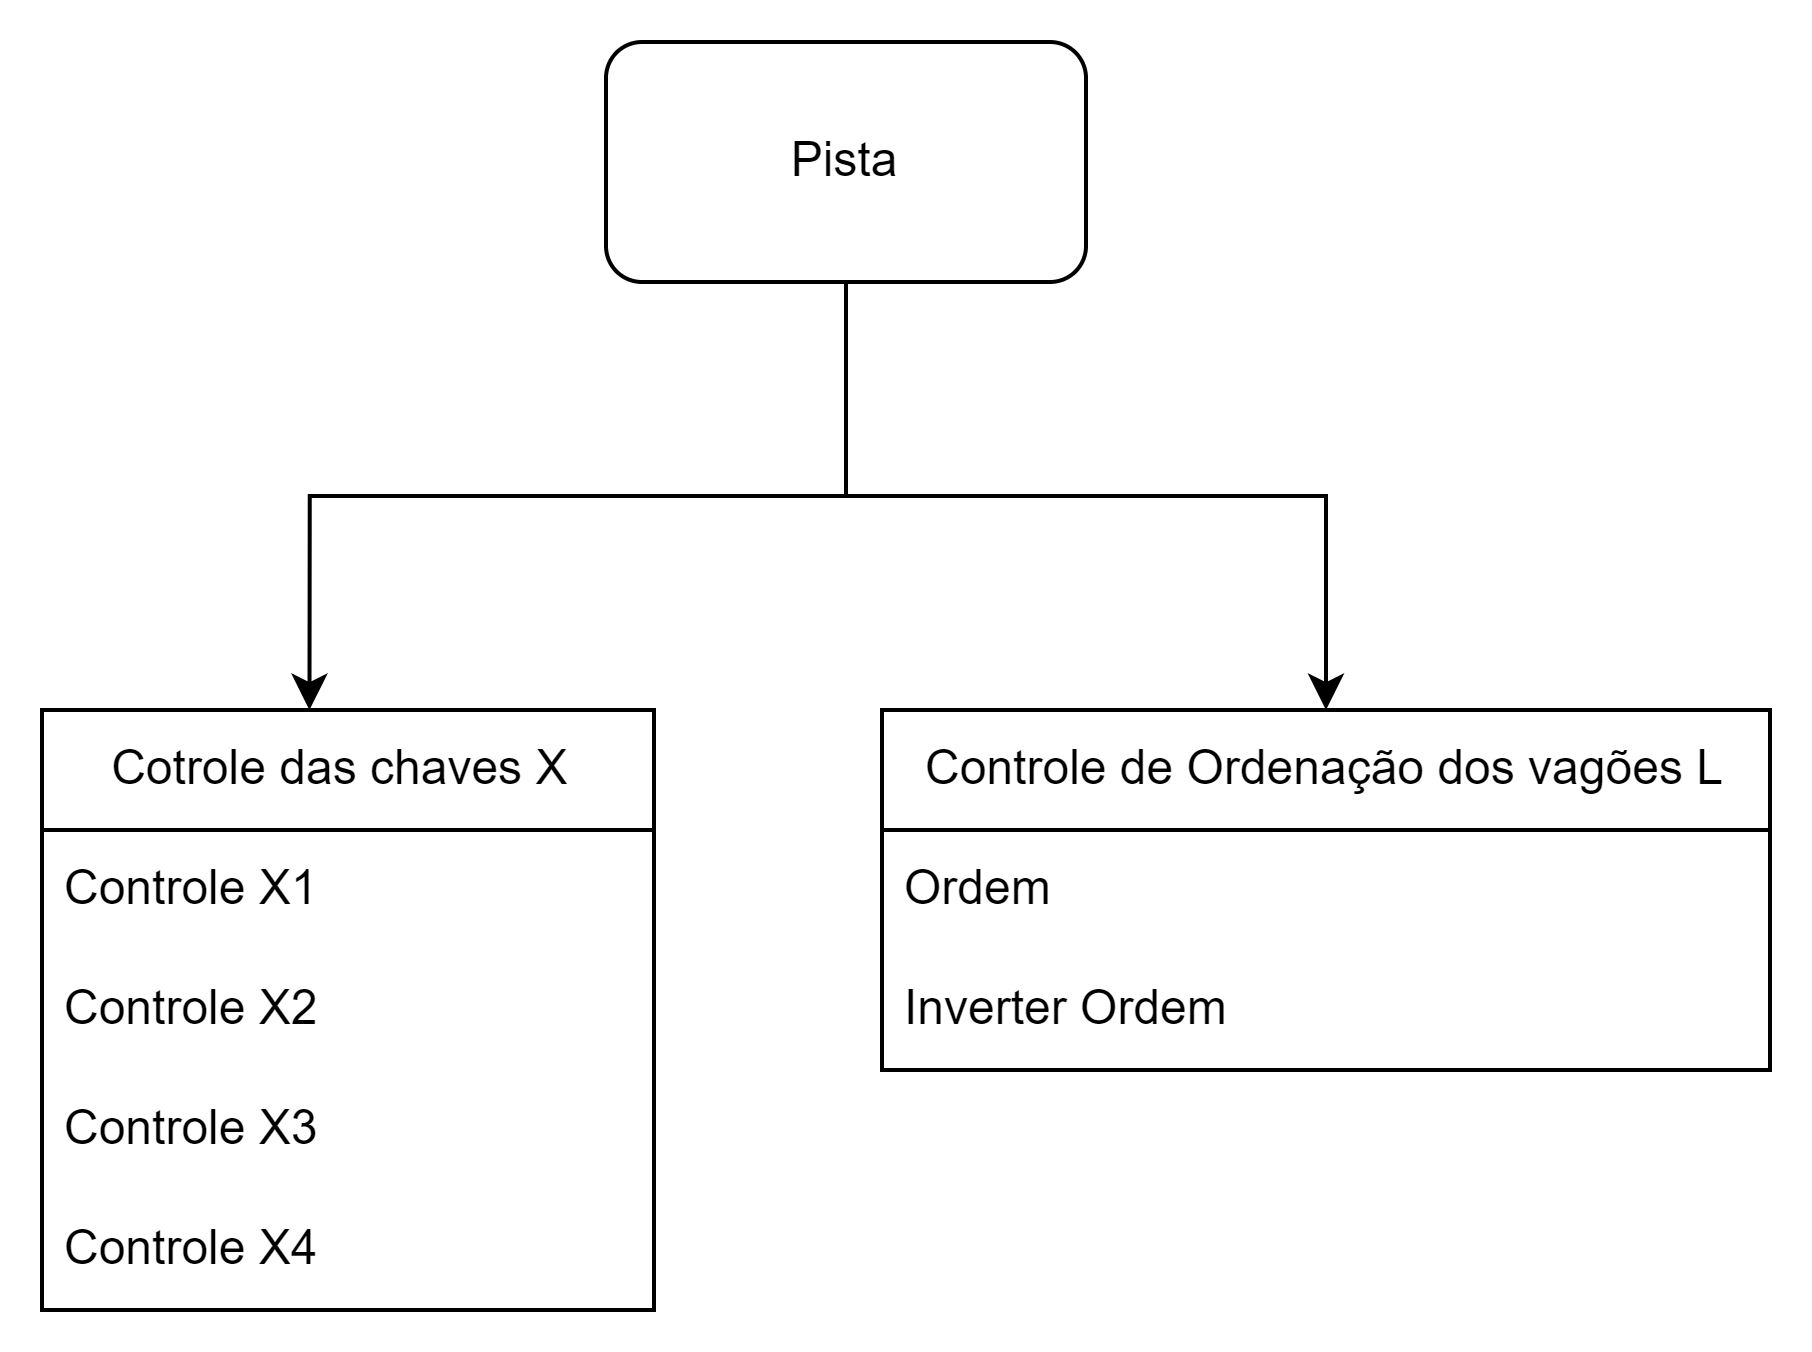
\includegraphics[width=0.8\linewidth]{figures//Simulation//Modelagem/hierarquia.png}
    \legend{Fonte: Elaborado pelo autor.}
\end{figure}

A RPC de camada superior é dada pela figura \ref{fig:rede_geral}, nela é possível verifica a existência de outras sub-redes dada pelas transições \textit{Controle} $X_1$ a $X_4$ e \textit{Ordem} e \textit{Inverter Ordem}, dadas pelas transições com dupla bordas, que correpondem aos componentes de mais baixa hierarquia modelado através da figura \ref{fig:hierarquia_RPC}.

\begin{figure}[ht]
    \centering
    \caption{Rede de Nível Hierárquico superior}
    \label{fig:rede_geral}
    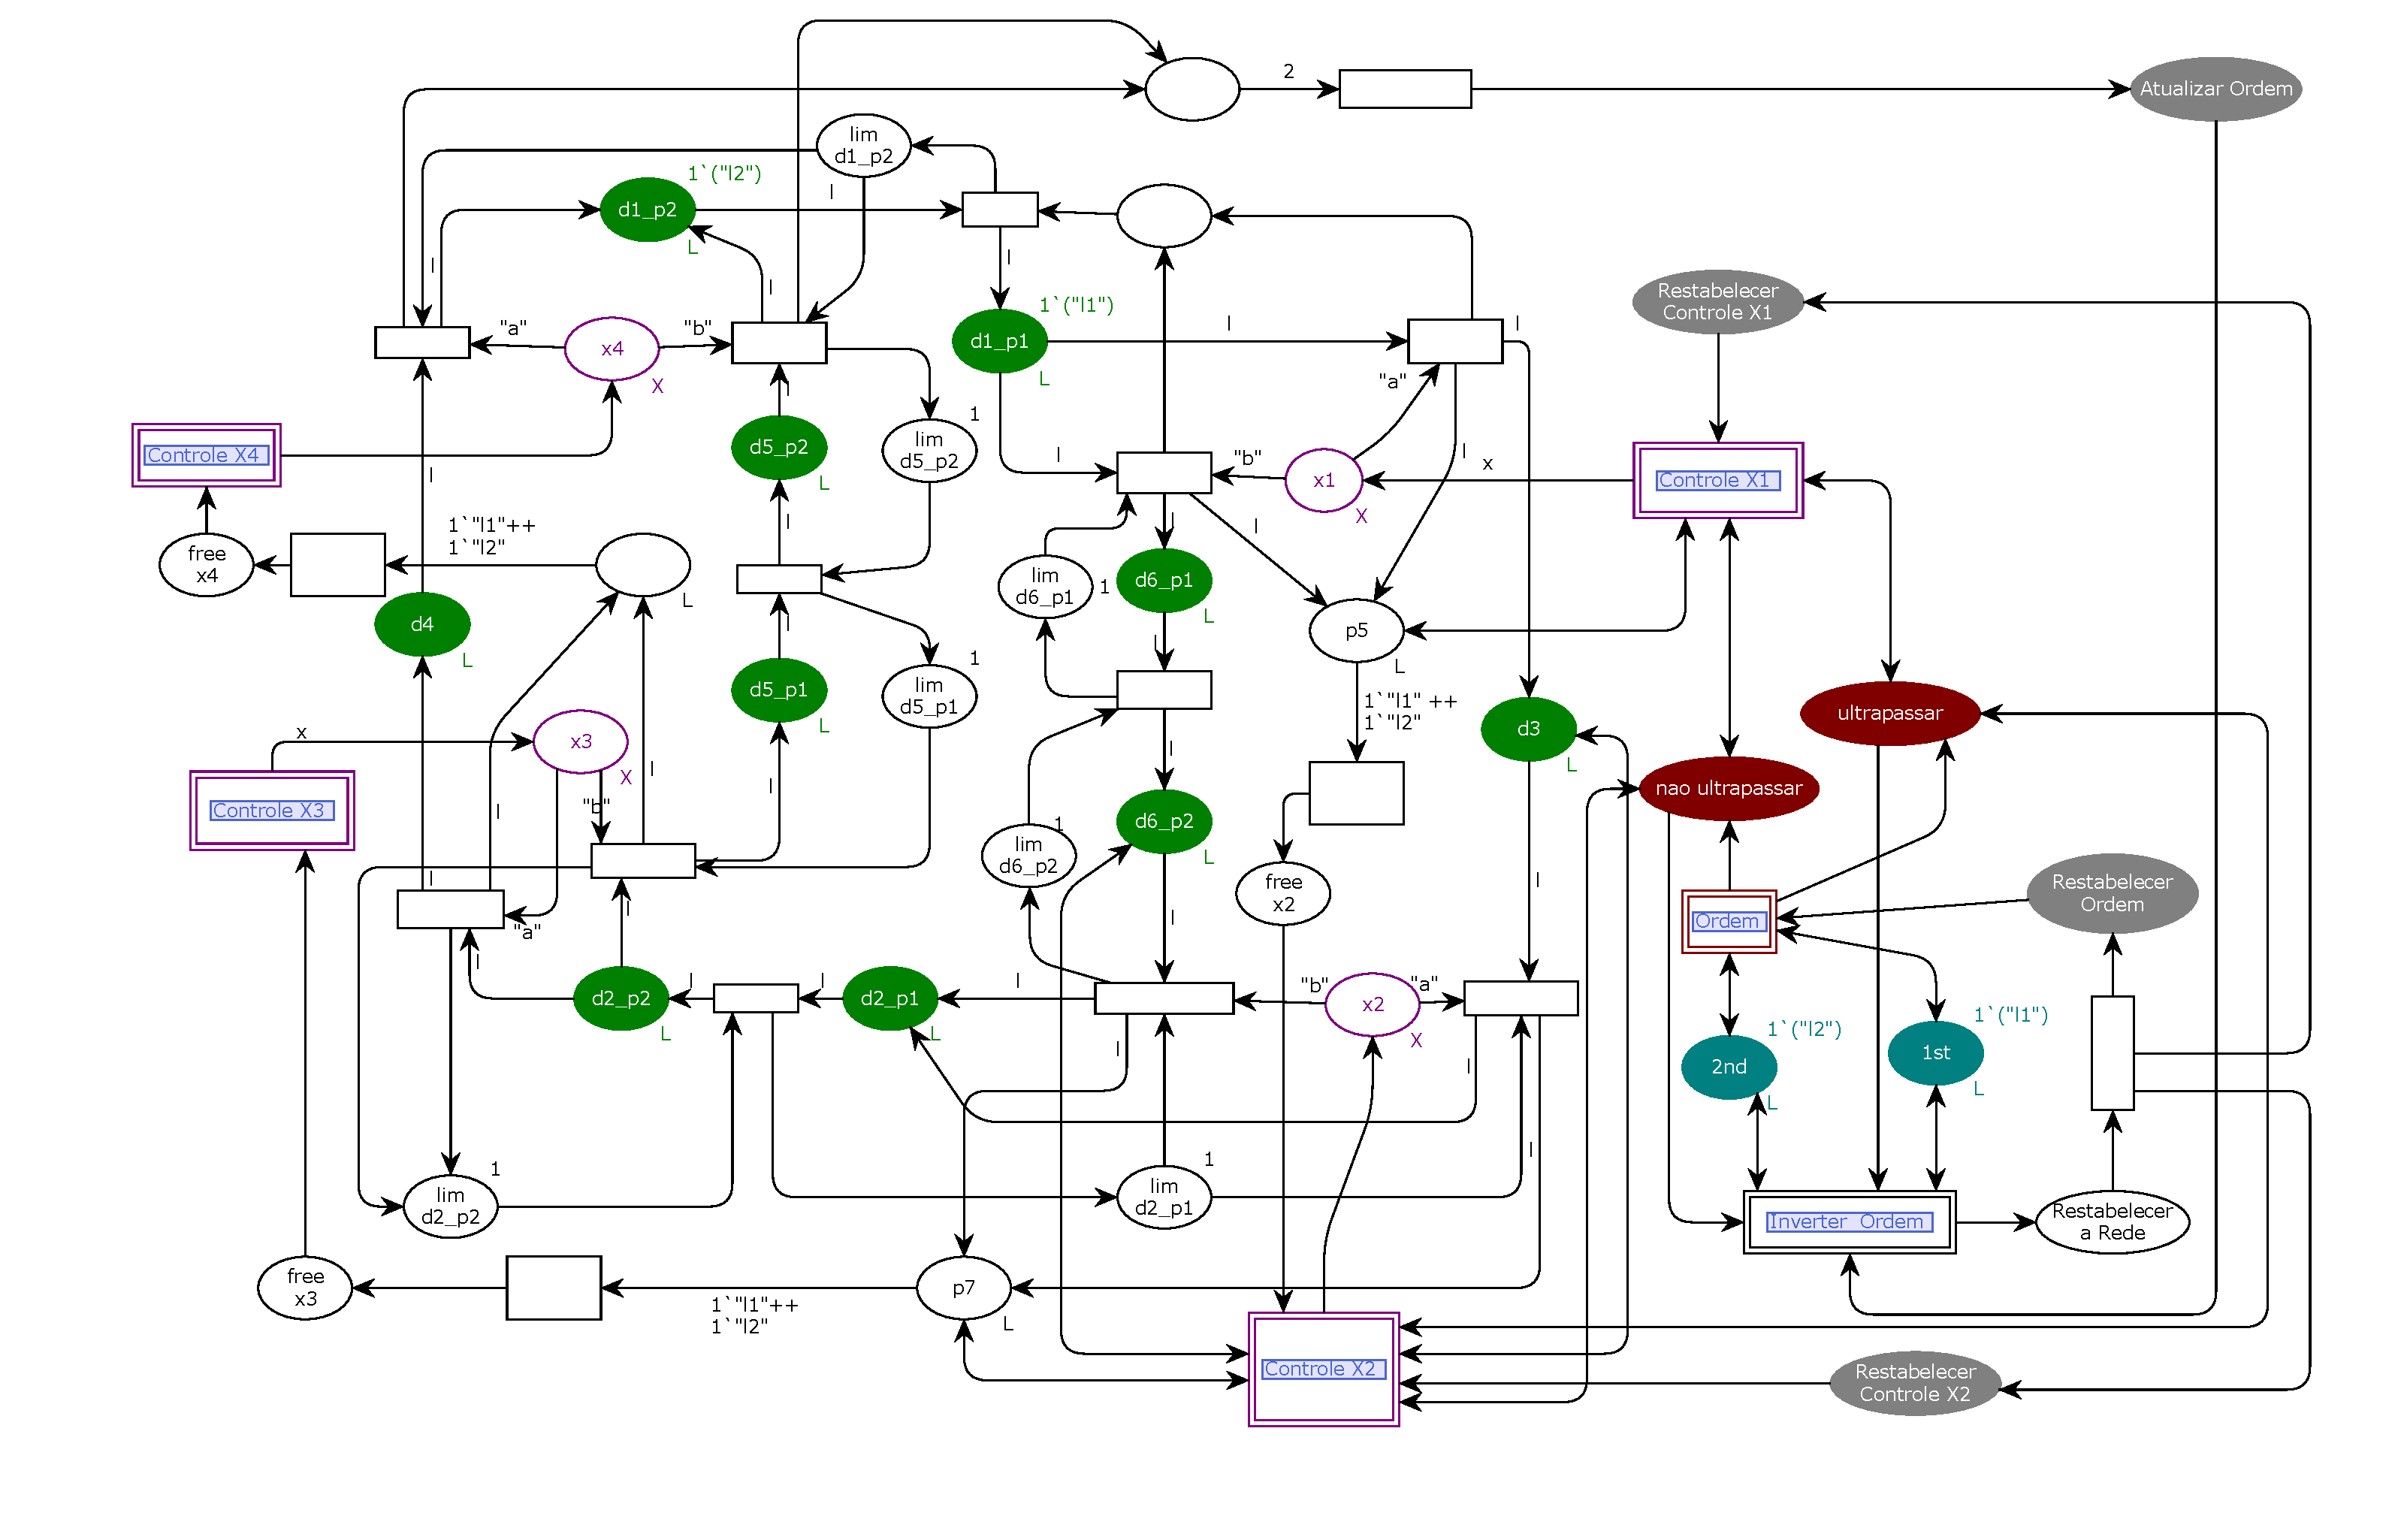
\includegraphics[width=1\linewidth]{figures/Simulation/Modelagem/rede_geral.eps}
    \legend{Fonte: Elaborado pelo autor.}
\end{figure}


\subsubsection{Modelagem da Pista}
\label{sub:model_pista}
A modelagem da pista foi feito através do conjunto de lugares e transições que representam o movimento e mecanismos pelos quais os vagões iram transitar, a modelagem completa dada pela figura \ref{fig:rede_geral} foi dividida em algumas máscaras (representação parcial da rede) para melhor visualização ao longo da sub seção. 

A figura \ref{fig:pista_RPC} demonstra os principais componentes das pista, tal que os lugares de $d_1$ a $d_6$ referem-se as curvas da pista representada na figura \ref{fig:pista_com_dois_agentes}. Observe que o conjunto de cores nesses lugares são o conjunto $L$, indicando que neles transitam as fichas do tipo vagões que podem ser "$l_1$" ou "$l_2$" como nos casos do lugar $d_1\_p_1$ e $d_1\_p_2$ respectivamente. Assim de modo análogo os arcos que referentes a movimentação das fichas do tipo \textit{L} são da variável tipo \textit{l} que controla os graus de saída e entrada das transições que movimentam os vagões ao longo da pista. Também é modelado os locais de junções e divisões, por exemplo no lugar $d_1\_p_1$ que representa a área $1$ da pista $d_1$ nela a pista sofre uma divisão, de modo que o vagão pode ir ou para a curva $d_6$ ou para a curva $d_3$ da pista. Os locais de junção ocorrem por exemplo na curva $d_2\_p_1$ da pista, em que recebe tanto os vagões que veem da pista $d_3$, quanto da pista $d_6$.
\begin{figure}[ht]
    \centering
    \caption{Máscara dos Componentes da pista na RPC}
    \label{fig:pista_RPC}
    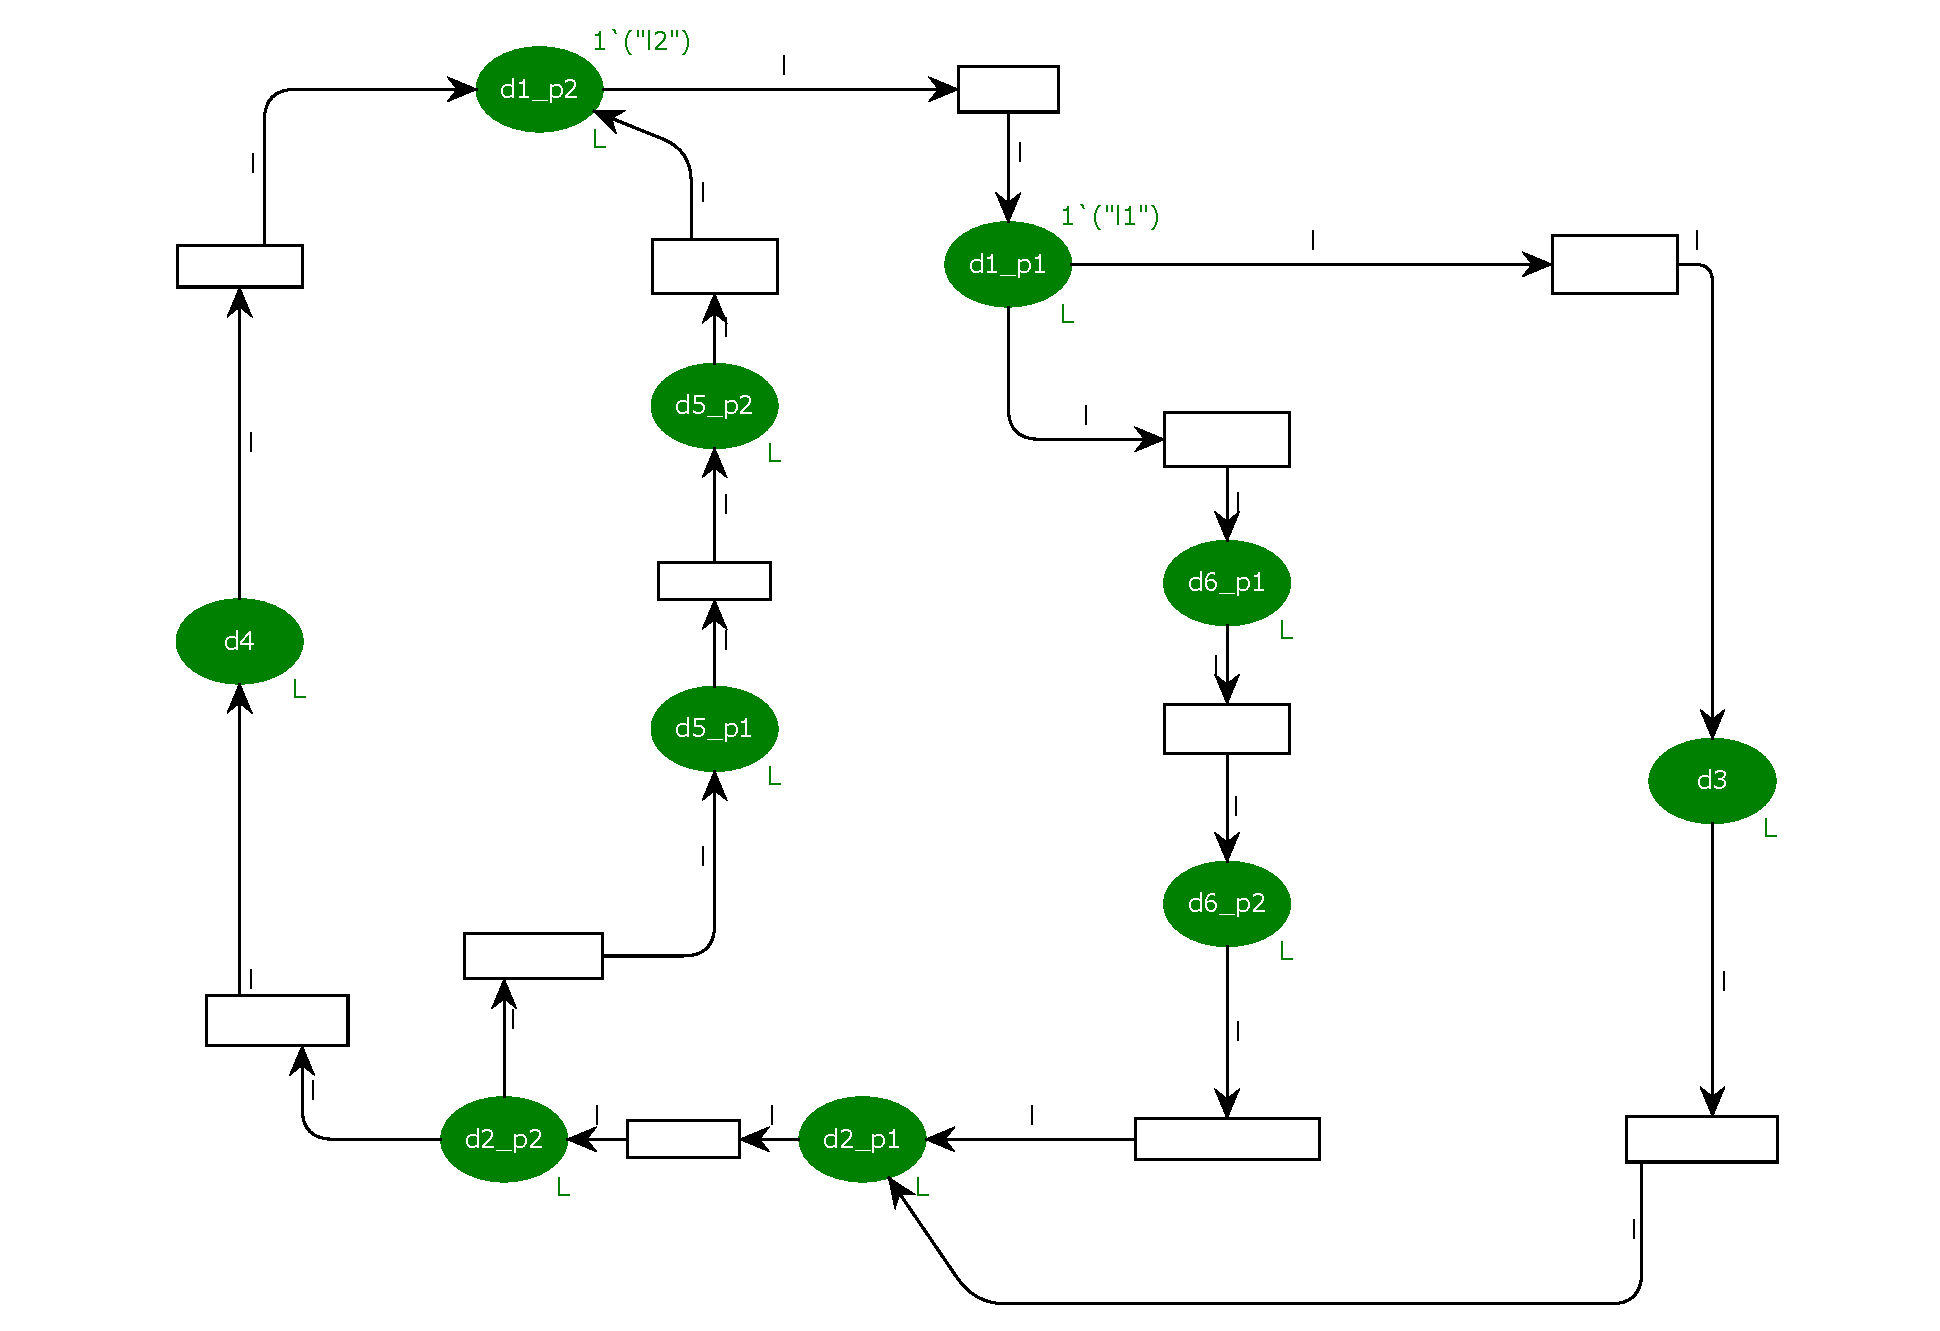
\includegraphics[width=1\linewidth]{figures//Simulation//Modelagem/pista.eps}
    \legend{Fonte: Elaborado pelo autor.}
\end{figure}

Para a modelagem da pista também é importante a implementação do conceito limitadores de região, que são lugares que controlam a quantidade de vagões por região, que para níveis de modelagem na RPC são importantes para evitar que dois vagões estejam na mesma região ao mesmo tempo. Os limitadores de região são implementados em algumas regiões como demonstrado na figura \ref{fig:limitadores_pista}, de modo que quando o vagão entra em determinada região é retirado uma ficha do lugar \textit{lim} ${d_x\_p_y}$, desabilitando a transição que permite a entrada de um vagão naquela região, tal ficha é devolvida quando o vagão que está sai para outra região. 

Por exemplo, note que para que uma ficha entre no lugar $d_5\_p_2$ é necessário que haja uma ficha no lugar \textit{lim} $d_5\_p_2$, e que ao entrar nessa região uma ficha é consumida e ao sair a ficha é retornada ao limitador garantido que somente um vagão ocupara aquela região por vez.

\begin{figure}[ht]
    \centering
    \caption{Máscara dos Componentes da pista com o controle das chaves na RPC}
    \label{fig:limitadores_pista}
    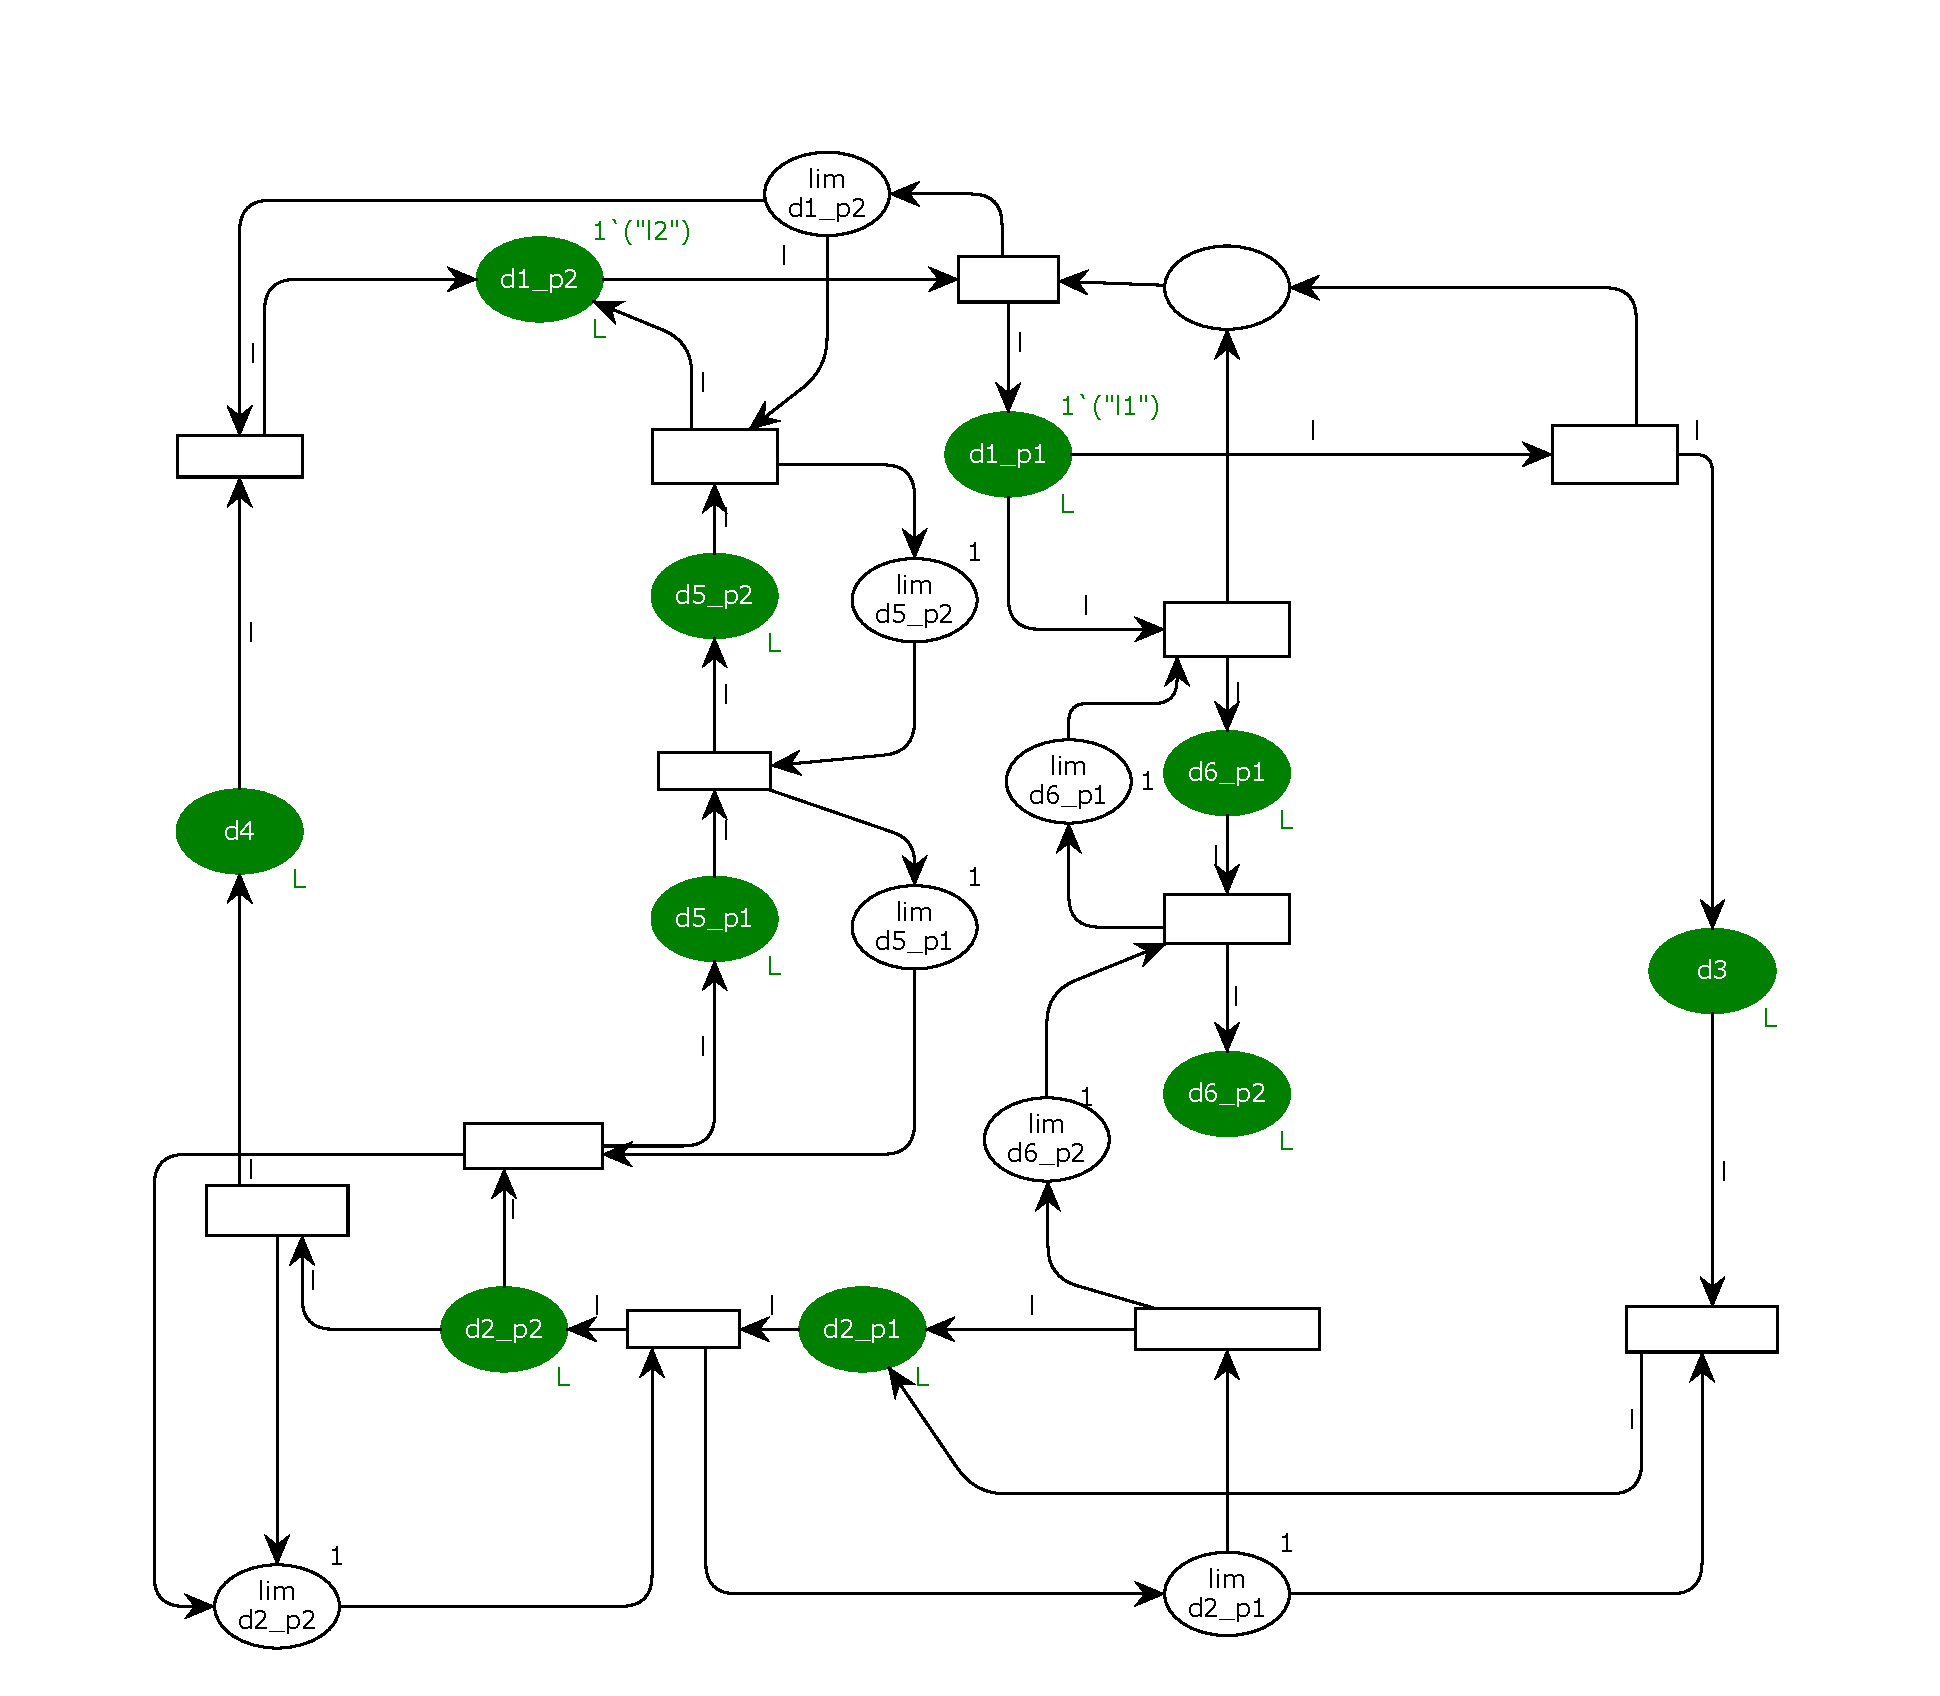
\includegraphics[width=1\linewidth]{figures//Simulation//Modelagem/limitadores_pista.eps}
    \legend{Fonte: Elaborado pelo autor.}
\end{figure}

Outro conceito fundamental na modelagem de uma RPC é o de reestabelecimento da rede, garantido que ao chegar no final do ciclo de uma volta a rede continue em funcionamento para um número ilimitado de iterações, tal reestabelecimento é demonstrado na figura \ref{fig:restabelecer_geral}. Note que após a segunda ativação da chave $X_4$ é dado o comando de atualizar a ordem vigente dos vagões e logo em seguida é dado o comando de \textit{Reestabelecer a Rede}, enviando a ficha para reestabelecer os \textit{Controles} $X_1 e X_2$ assim como o \textit{Controle de Ordem}.

\begin{figure}[ht]
    \centering
    \caption{Máscara dos Componentes de reestabelecimento na RPC}
    \label{fig:restabelecer_geral}
    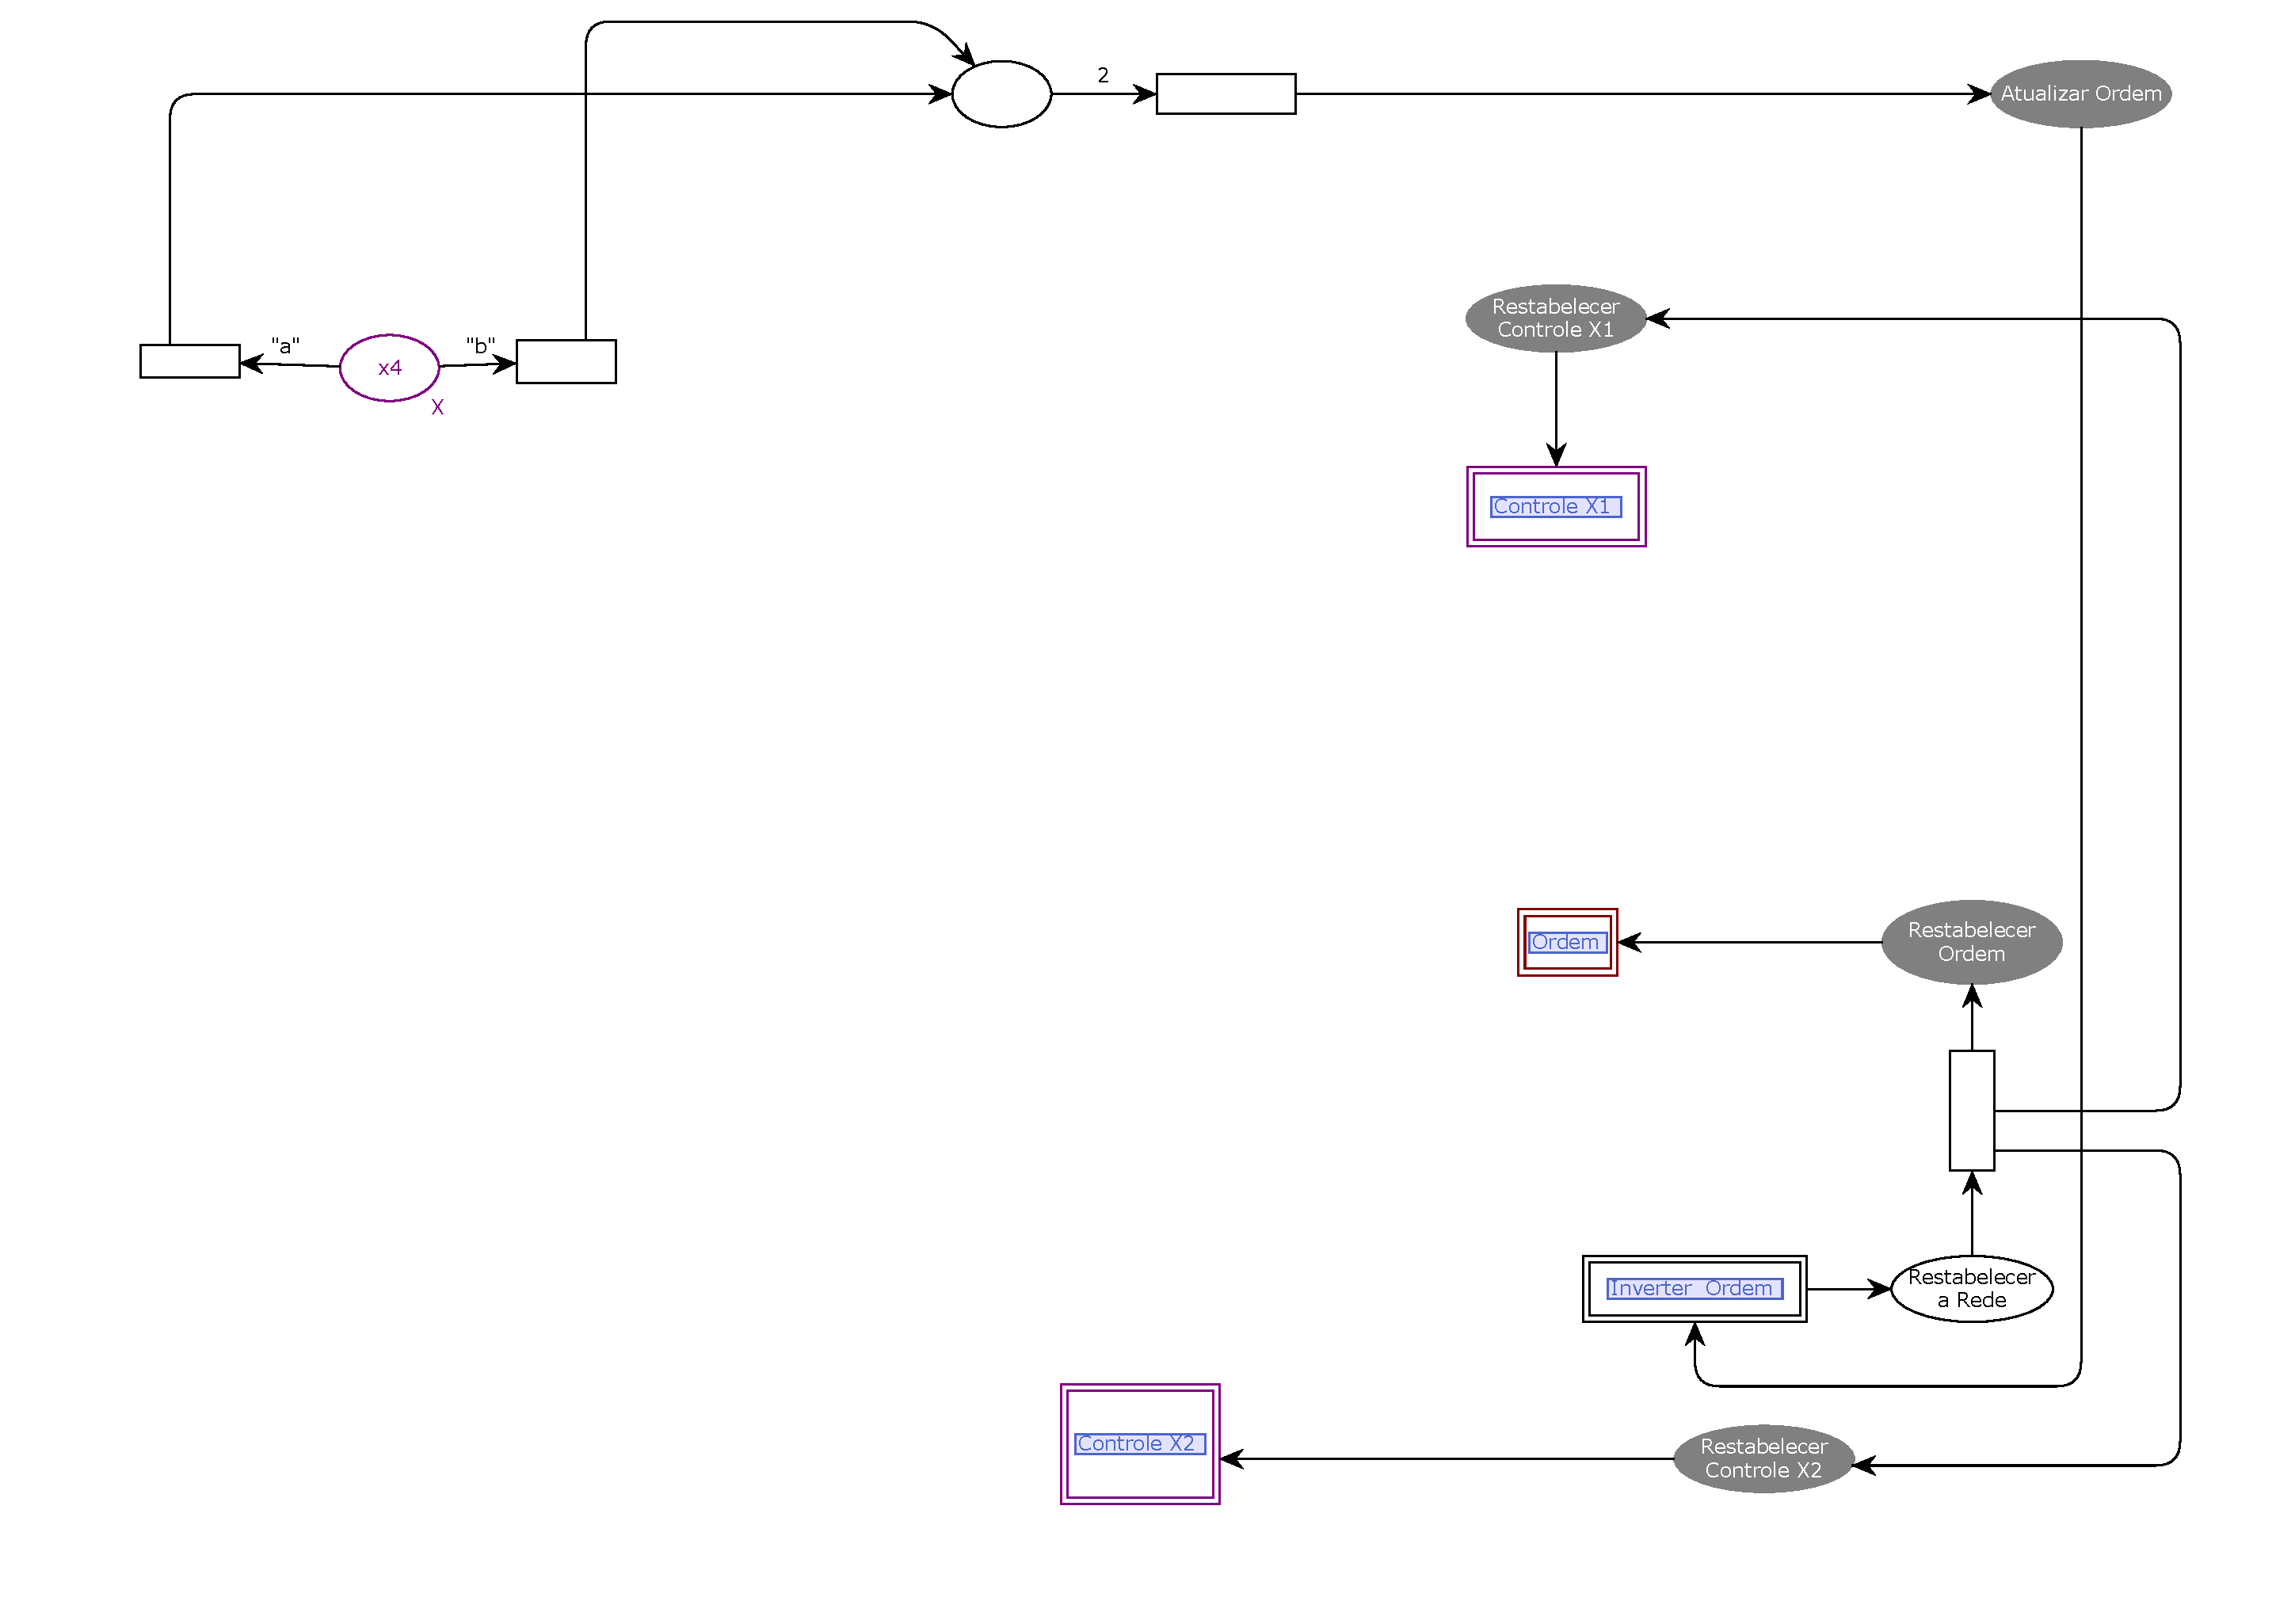
\includegraphics[width=1\linewidth]{figures/Simulation/Modelagem/restabelecer_geral.eps}
    \legend{Fonte: Elaborado pelo autor.}
\end{figure}

\clearpage
\subsubsection{Modelagem Controladores}
Considerando o modelo anterior na subseção \ref{sub:model_pista} de organização das pistas a figura \ref{fig:pista_chaves_RPC} representa além dos componentes fundamentas das curvas das pistas $d_1$ a $d_6$, os componentes de chaves \textit{X}, com as transições hierárquicas de \textit{Controle} $X_1$ a \textit{Controle} $X_4$. Observe que nos pontos de junção e divisão se encontroam os locais $X_1$ a $X_4$, que pertencem ao conjunto \textit{X} que podem receber fichas do tipo "a" ou "b" como explicado no quadro \ref{qua:variaveis_RPC}, tais lugares controlam as condições de acionamento das transições ligadas os arcos de saída. 

Por exemplo, dado um ficha "1`$(l_1)$" no lugar $d_1\_p_1$ quem vai definir qual transição será habilita, se para ir para a pista $d_3$ ou para a pista $d_6$, será a ficha no lugar $x_1$, que é controlada pela transição hierárquica \textit{Controle} $X_1$. Tal que dependendo da ficha que o local \textit{X} receber pelos respectivos Controladores será habilitada e desabilitada as transições que ligam as curvas ao longo da pista. 
\begin{figure}[ht]
    \centering
    \caption{Máscara dos Componentes da pista com o controle das chaves na RPC}
    \label{fig:pista_chaves_RPC}
    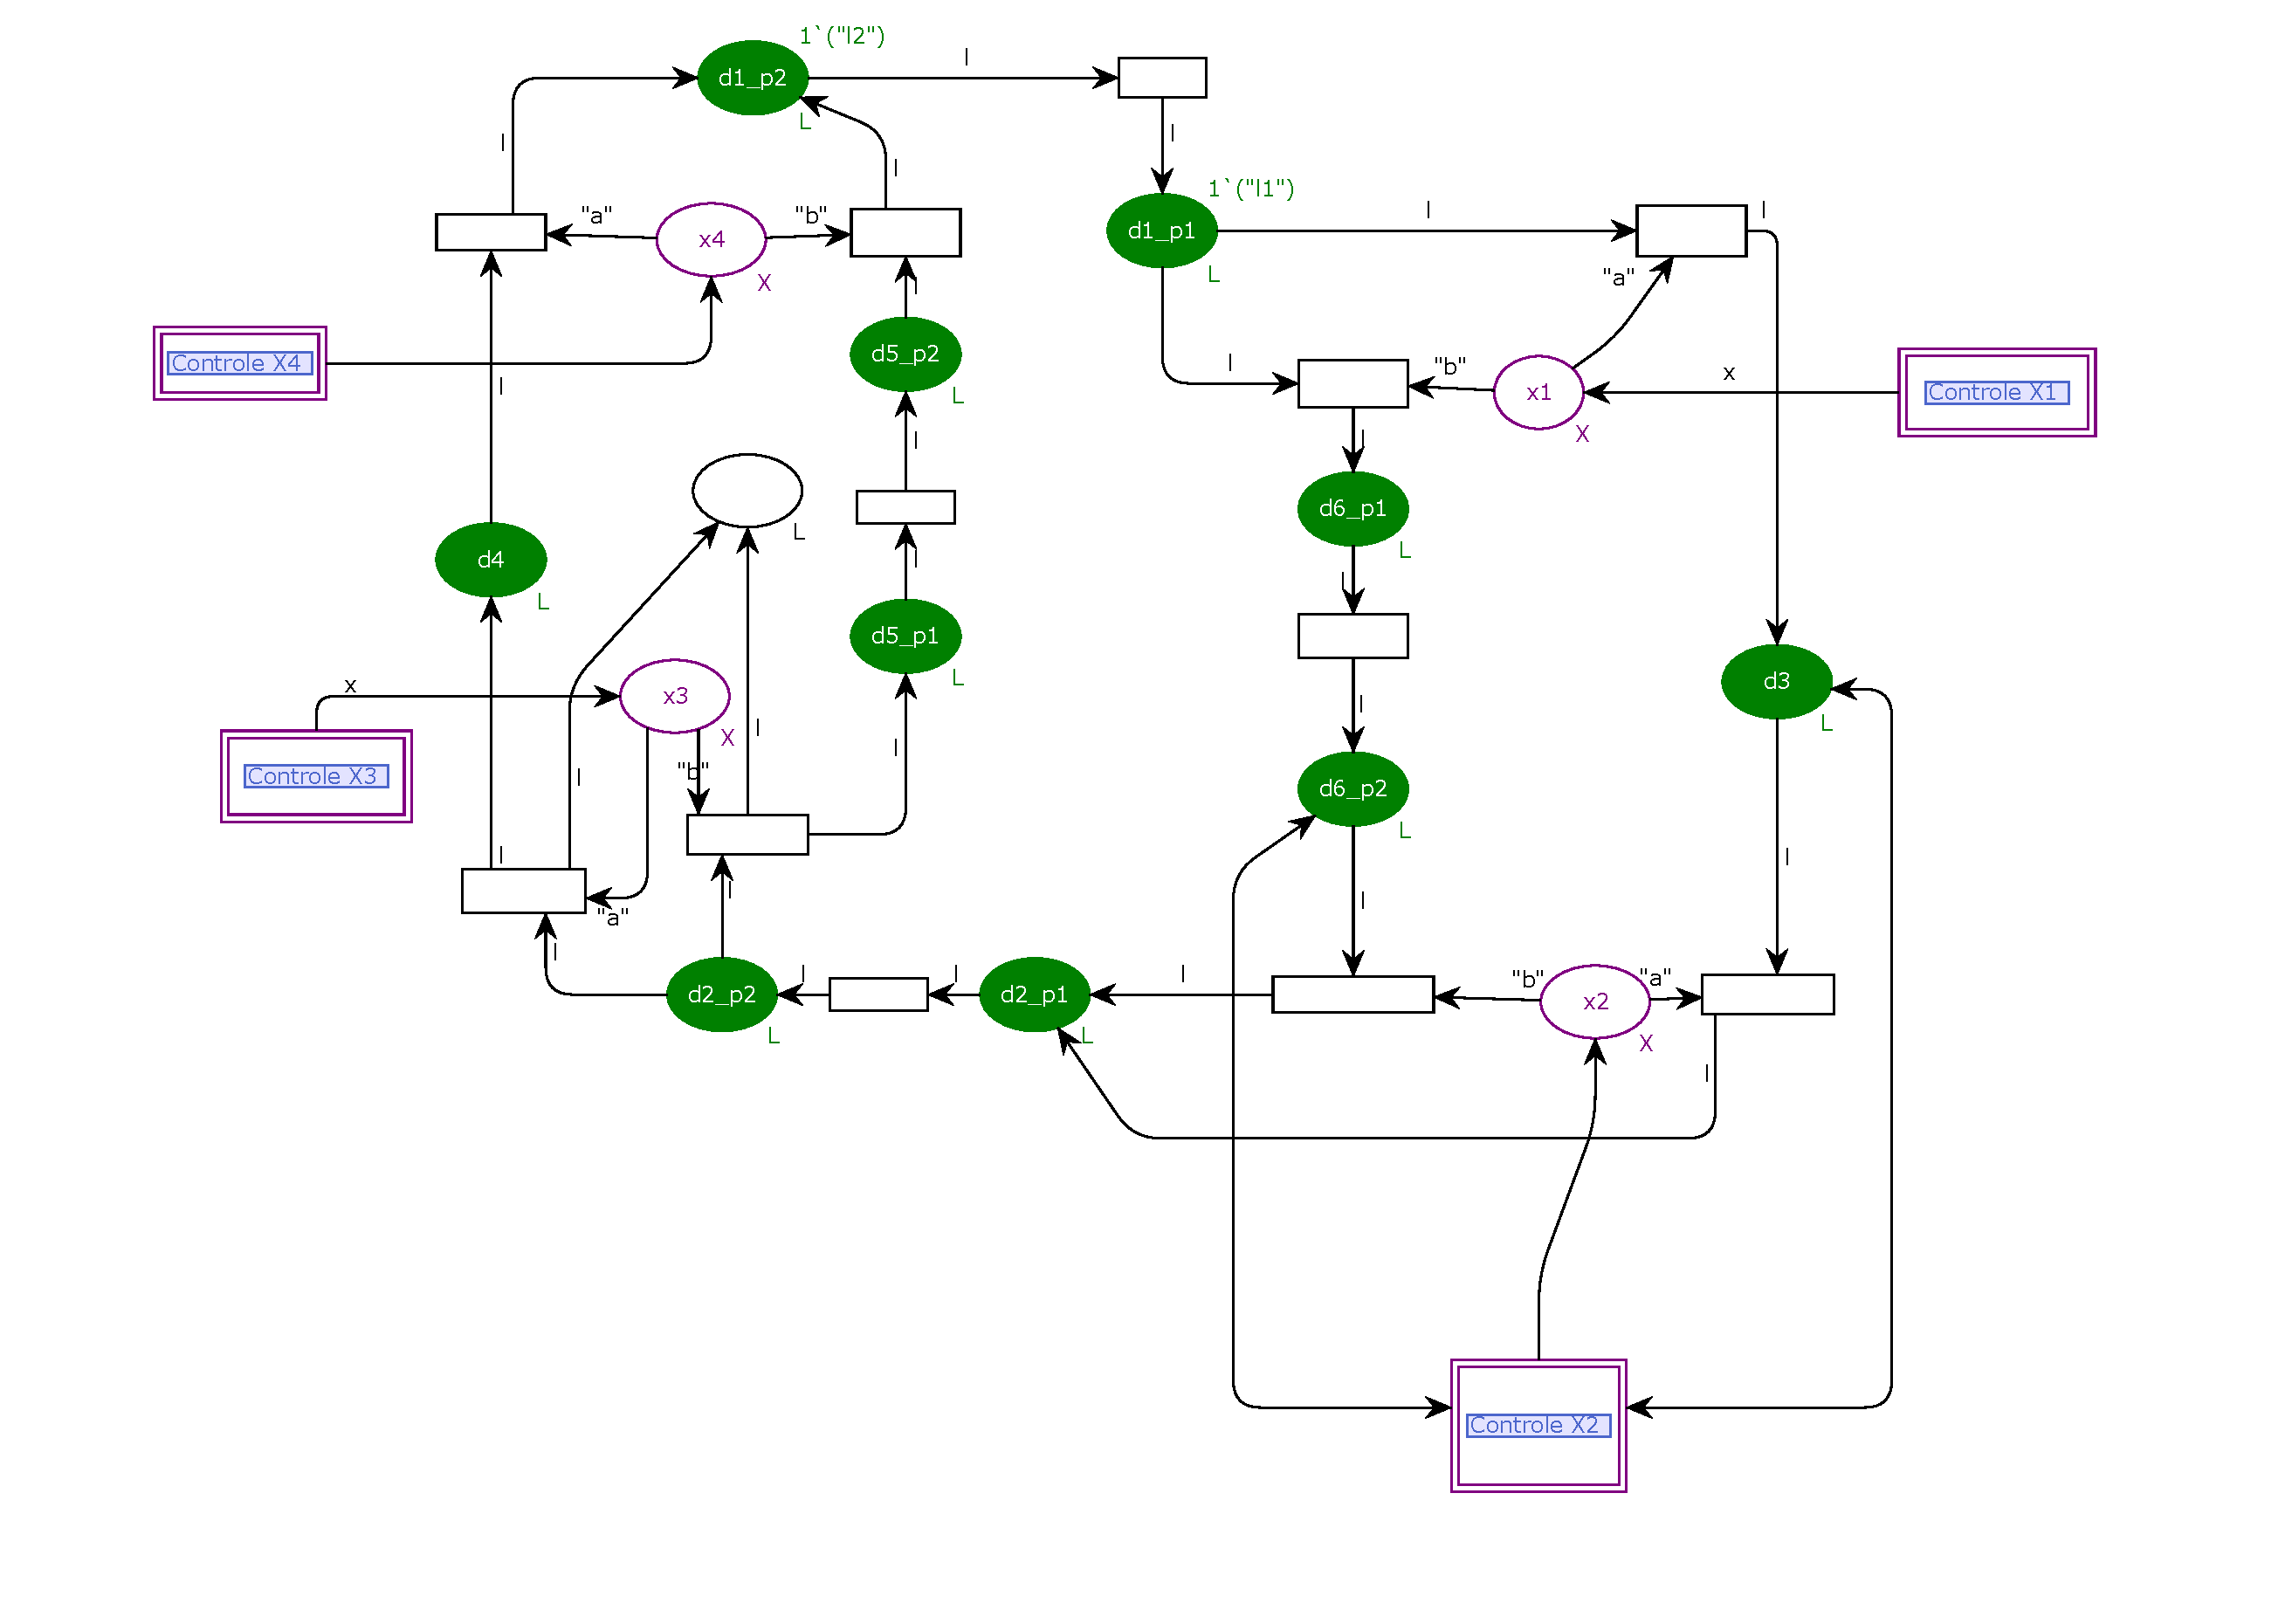
\includegraphics[width=1\linewidth]{figures//Simulation//Modelagem/pista_com_chaves.eps}
    \legend{Fonte: Elaborado pelo autor.}
\end{figure}

Na modelagem dos controladores, é essencial assegurar a comunicação entre os elementos da pista em certos momentos, permitindo que os controladores tomem decisões com base nas posições dos vagões. Um exemplo dessa comunicação é ilustrado na Figura \ref{fig:free_control}. Em algumas transições conectadas às chaves, a informação sobre qual vagão passou pela região é transmitida à medida que as transições são acionadas. Posteriormente, essas informações são fornecidas, direta ou indiretamente, aos controladores.

Por exemplo, note que nas transições ligadas ao lugar $X_2$ possuem lugar de saída definida no conjunto L, de modo que ao passar algum vagão naquela região, a informação de qual vagão passou é processada pelo \textit{Controle} $X_2$. Posteriormente ao se passar os dois vagões diferentes a transição ligada ao lugar \textit{free} $x_3$ é habilitada, transmitindo a informação de que já se passaram aqueles dois tipos de vagões naquela região, para a tomada de decisão do \textit{Controle} $X_3$.

\begin{figure}[ht]
    \centering
    \caption{Máscara dos Componentes de controle das chaves e comunicadores na RPC}
    \label{fig:free_control}
    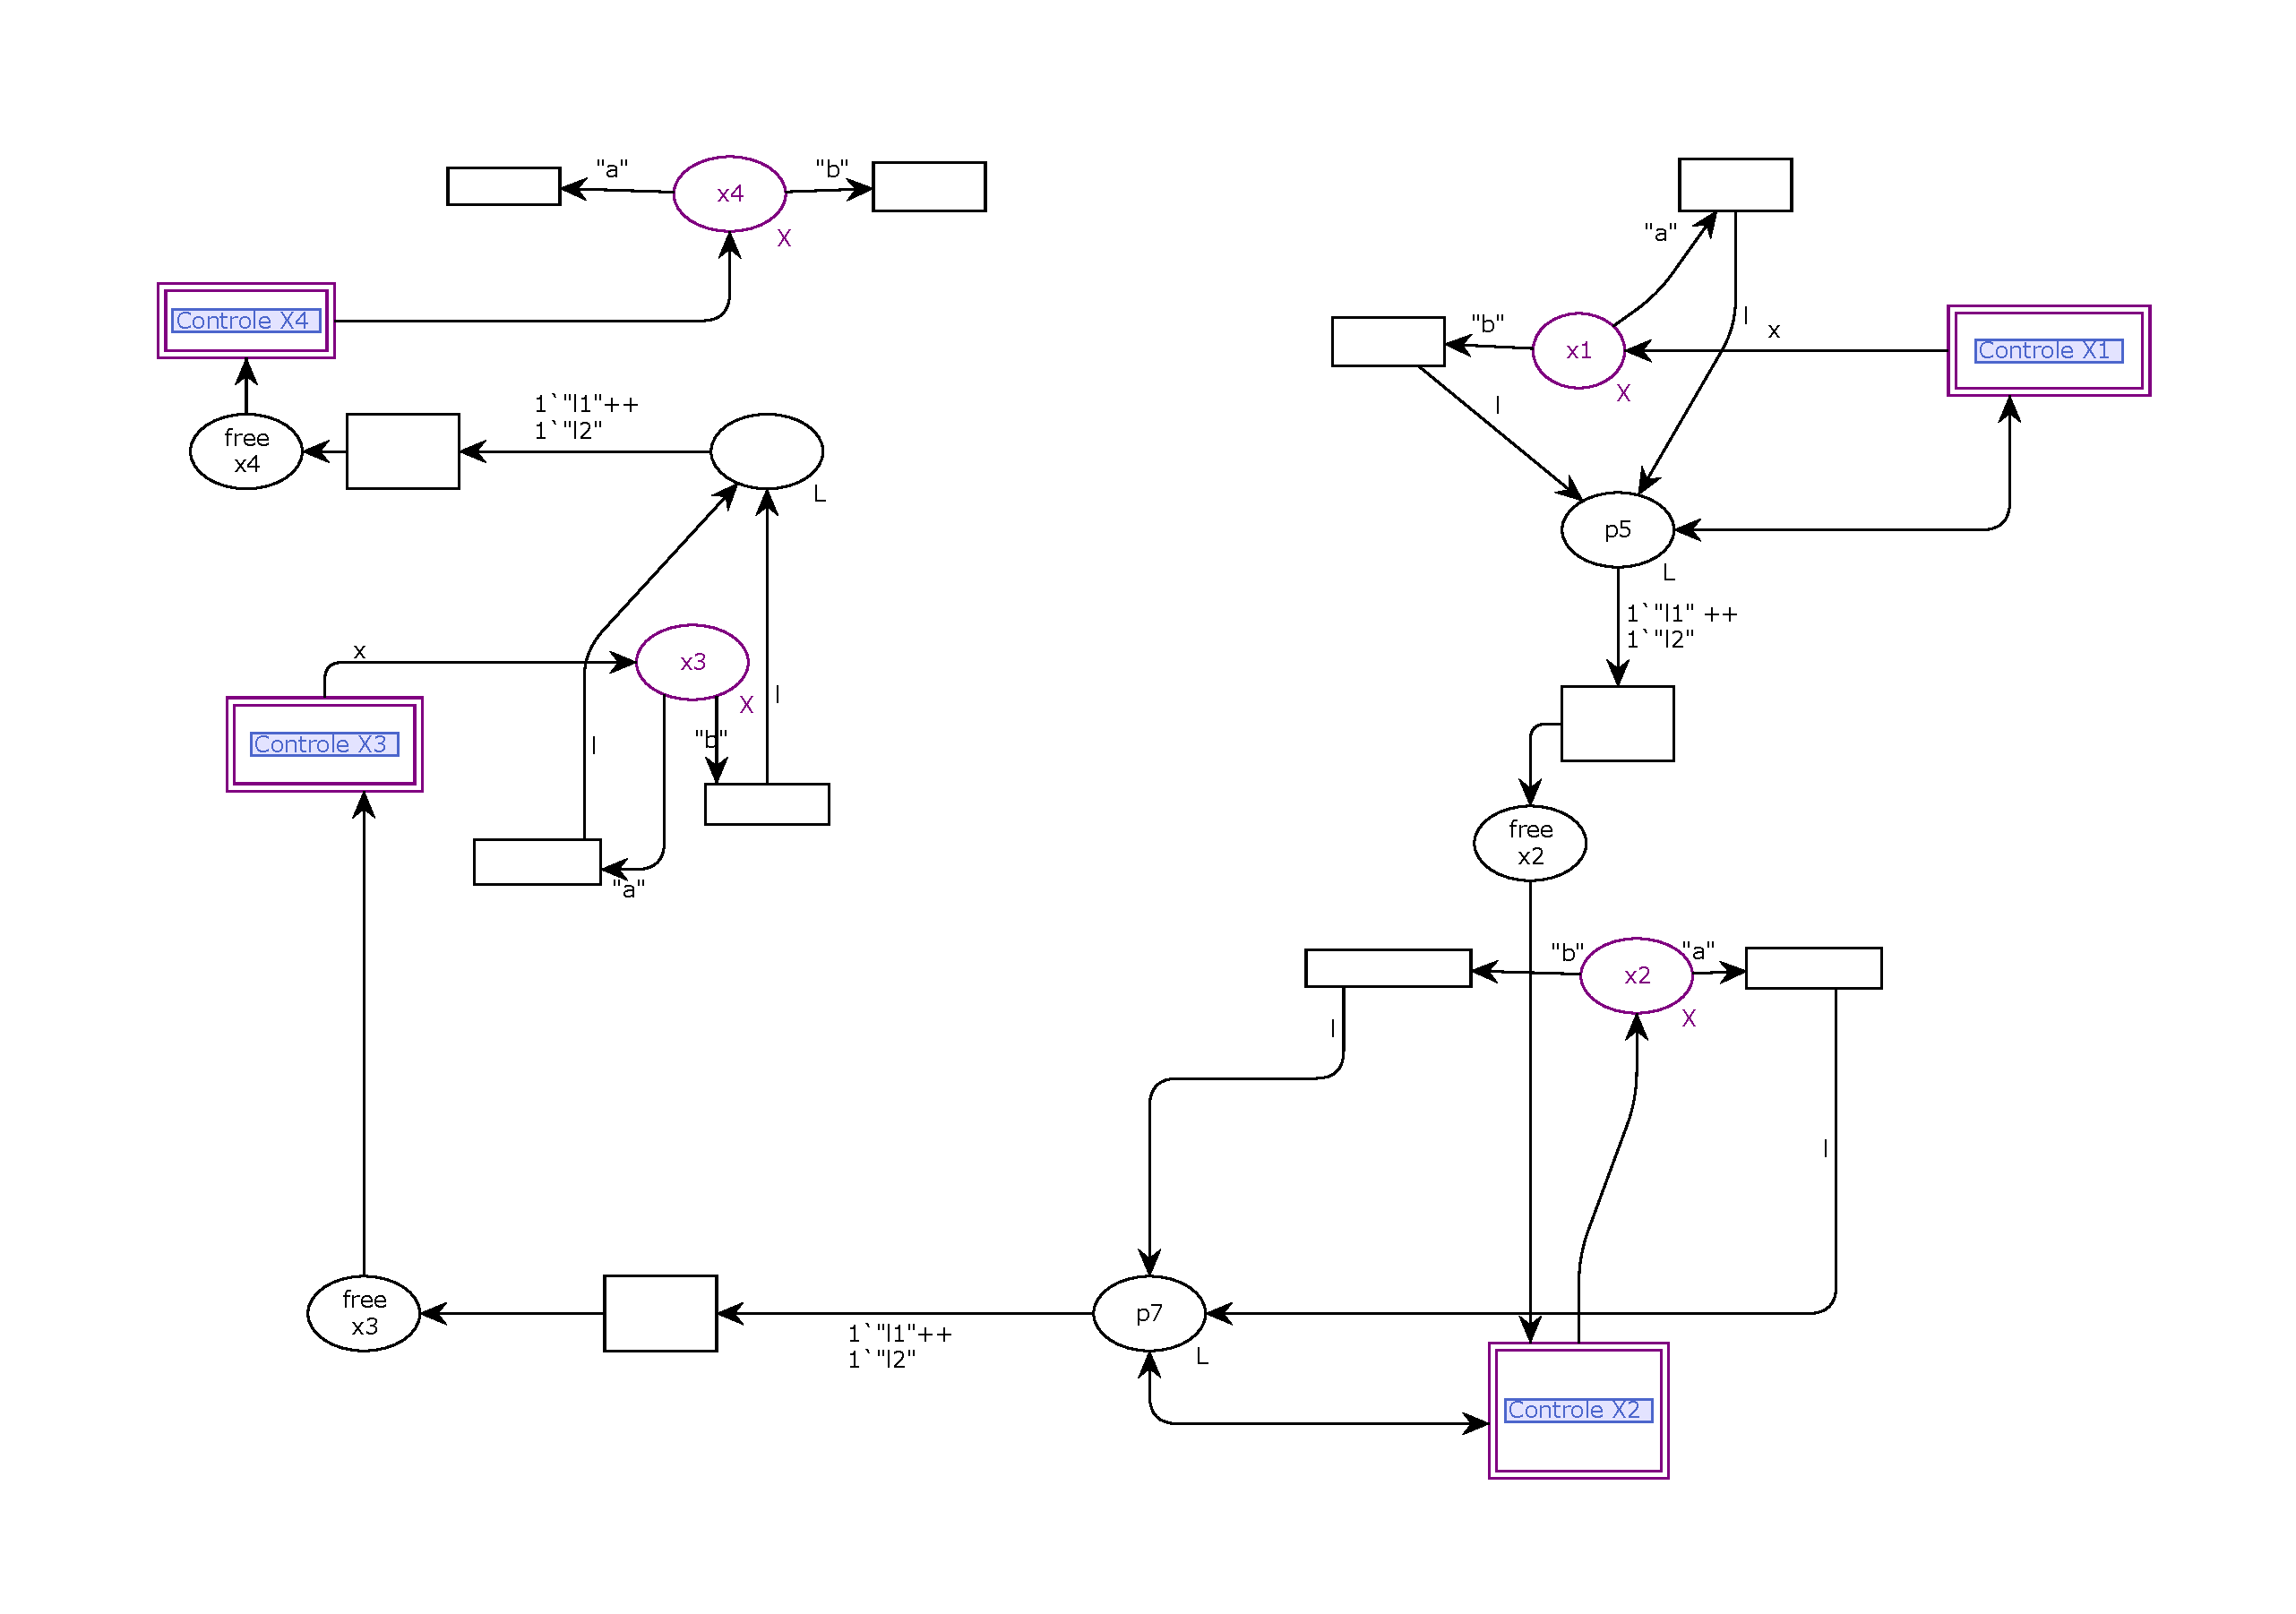
\includegraphics[width=1\linewidth]{figures//Simulation//Modelagem/free_control.eps}
    \legend{Fonte: Elaborado pelo autor.}
\end{figure}


Em um nível hierárquico abaixo do nível da pista, como demonstrado na figura \ref{fig:hierarquia_RPC} estão os \textit{Controladores} $x_1$ a $x_4$, que serão detalhados a seguir. 

O \textit{Controlador} $X_1$ referente a transição \textit{Controle} $X_1$ com borda vermelha na figura \ref{fig:free_control}, é demonstrado na figura \ref{fig:controle_x1}. Note que a rede de Controle de $X_1$, possui alguns lugares com subscrição denominadas de \textit{IN}, \textit{OUT} ou \textit{IN/OUT}, que são diretamente relacionadas aos lugares externos a rede, estabelecendo uma comunicação com lugares pertencentes ao nível hierárquico superior. Alguns lugares como $x1$ e $p5$ já foram demonstrados na máscara de componentes na figura \ref{fig:free_control}, outros serão demonstrados na subseção \ref{sub:model_ord} referente a modelagem de ordenação dos vagões.

Para o controle do lugar $X_1$ note que a rede possui inicialmente uma ficha no lugar $p_1$, de modo que dependendo do comando de ultrapassar ou não ultrapassar a transição $t_2$ ou $t_1$ será acionada, respectivamente. O acionamento primeiro coloca ficha de posição "a" ou "b" na chave $X_1$ e posteriormente a posição "b" pela transição $t_3$ pós a passagem do primeiro vagão sinalizada pelo lugar $p_5$. Após os dois comandos de posição serem utilizados a rede aguarda o comando externo de restabelece o controle para assim, reiniciar a rede para o estado inicial e começar um novo ciclo.

\begin{figure}[ht]
    \centering
    \caption{Rede referente ao controle hierárquico X1 na RPC}
    \label{fig:controle_x1}
    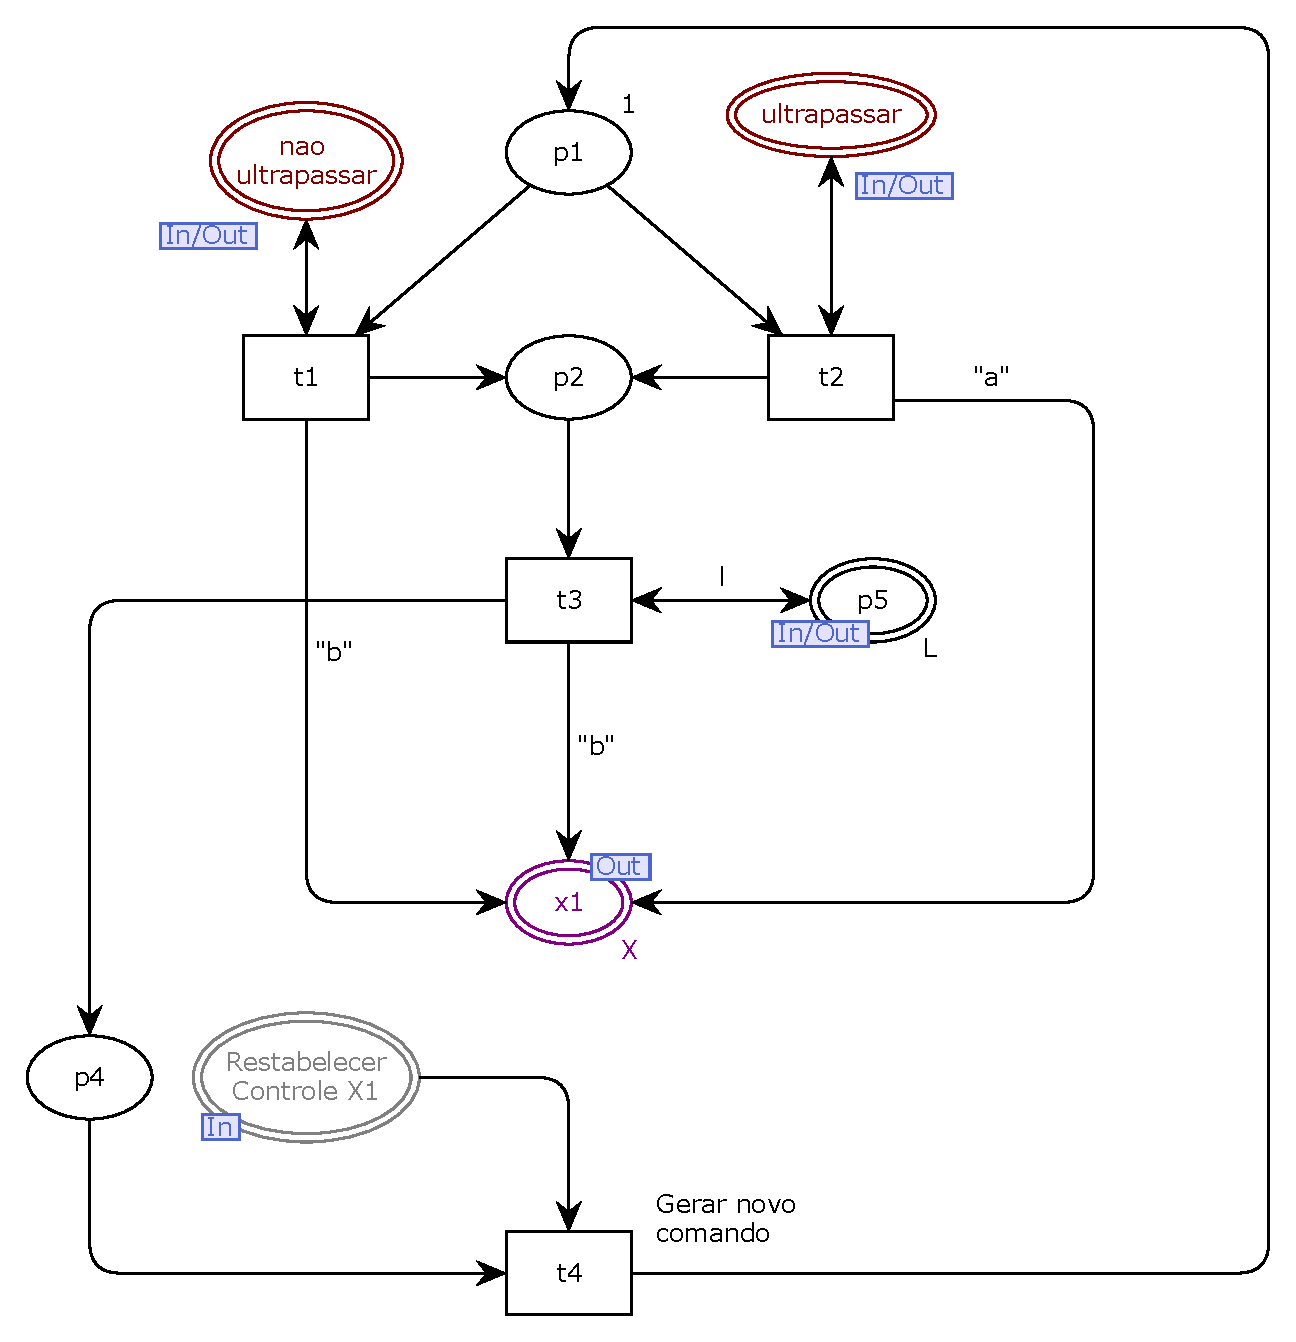
\includegraphics[width=0.8\linewidth]{figures//Simulation//Modelagem/controle_x1.eps}
    \legend{Fonte: Elaborado pelo autor.}
\end{figure}

A RPC referente a transição \textit{Controle} $X_2$ é demonstrado na figura \ref{fig:controle_x2}. Tal controle tem como objetivo primeiramente receber o vagão da pista $d_6$, ou seja do menor caminho e posteriormente, analisar caso tenha tido o comando de ultrapassagem o próximo vagão é esperado na pista $d_3$, caso contrário virá novamente pela pista $d_6$. Para alcançar tal objetivo primeiramente a estrutura da rede recebe uma ficha vinda da pista de \textit{free} $x_2$ ativando a transição $t_9$ que espera o vagão chegar em $d_6$, ao ser identificado na curva é liberada primeiramente a ficha para X2 "b". Posteriormente, dependendo do comando relacionado à ultrapassagem é acionado $t_13$ ou $t_12$, com as fichas respectivamente em $p_11$ ou $p_10$, é esperado que chegar uma ficha no lugar $p_7$ indicando que já pode dar o segundo comando para a chave, por fim é dado o comando de posição "a" ou "b" para a chave caso $t_8$ seja acionado ou $t_7$, respectivamente. Ao fim do ciclo a rede espera uma ficha para restabelecer o \textit{Controle} $X_2$.

\begin{figure}[ht]
    \centering
    \caption{Rede referente ao controle hierárquico X2 na RPC}
    \label{fig:controle_x2}
    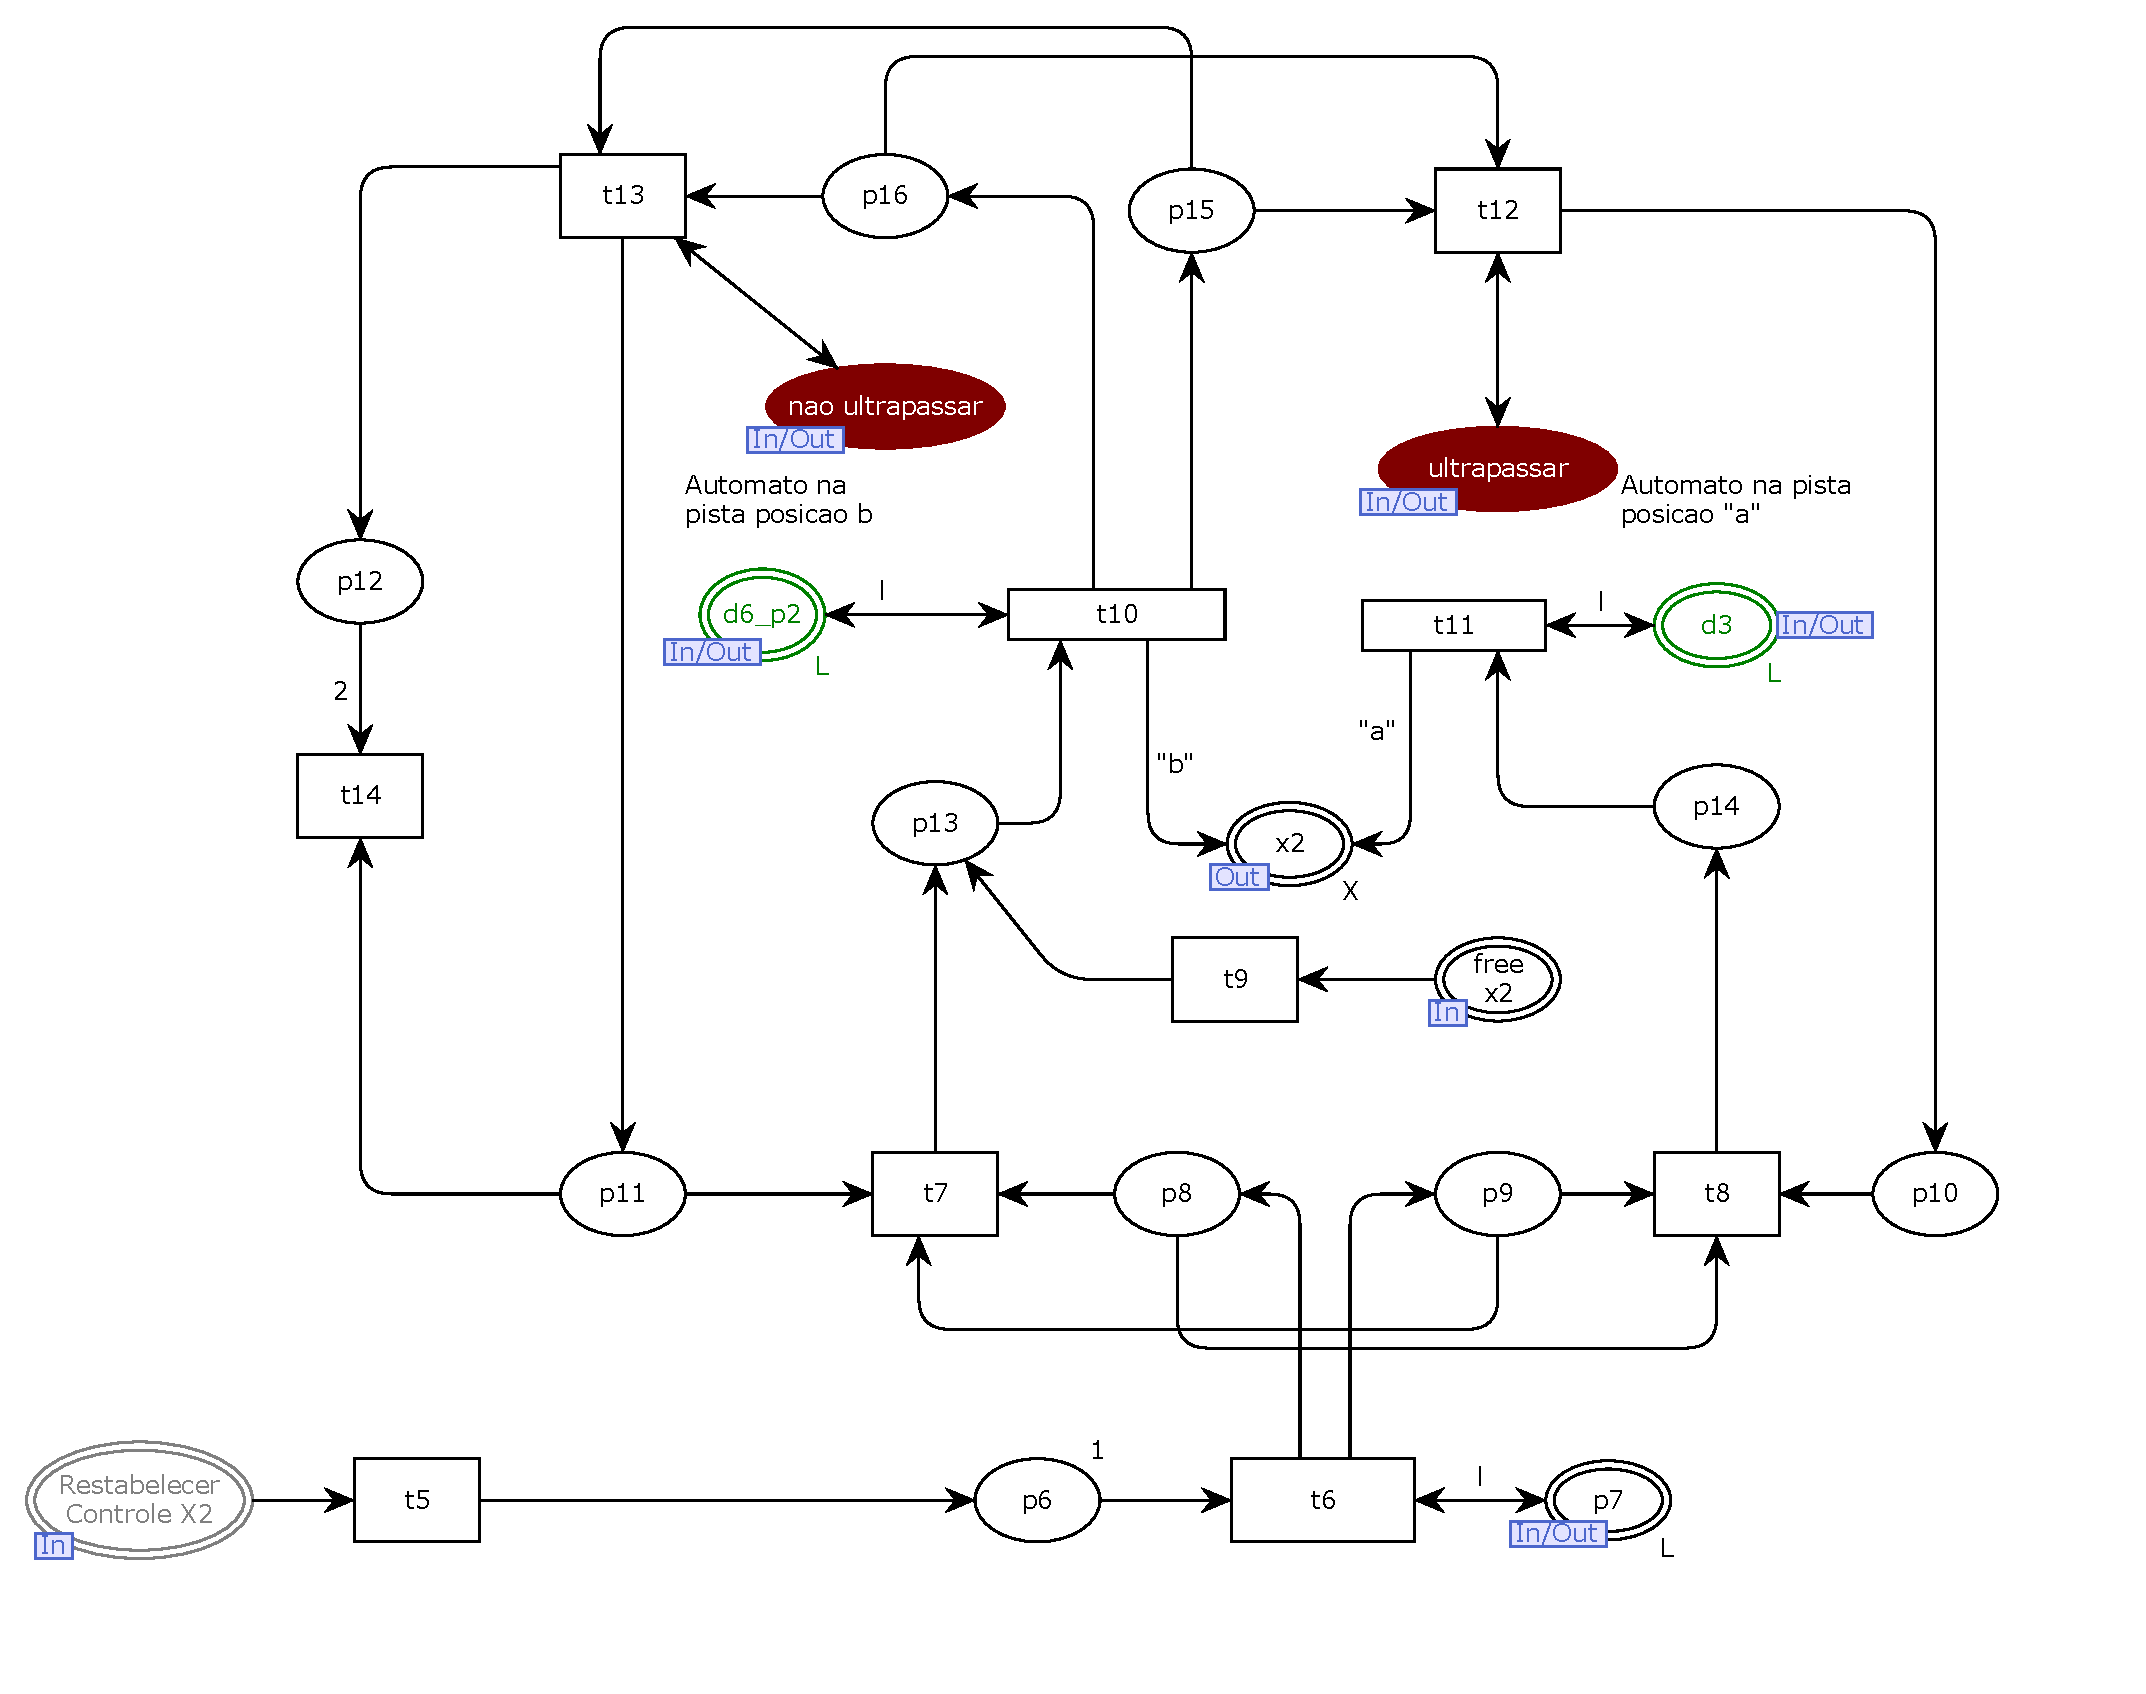
\includegraphics[width=1\linewidth]{figures//Simulation//Modelagem/controle_x2.eps}
    \legend{Fonte: Elaborado pelo autor.}
\end{figure}

A RPC referente ao controlador $X_3$ e $X_4$, possuem estruturas e comportamentos idênticos como demonstrados na figura \ref{fig:controle_x3} e \ref{fig:controle_x4}. Como no escopo da simulação o local de ultrapassagem foi fixado no \textit{Controle} $X_1$, o objetivo do \textit{Controle} $X_3$ e \textit{Controle} $X_4$ é apenas garantir que uma vez liberado o controle para o controlador através do lugar \textit{free} $x_3$ ou $x_4$ seja colocada a ficha de posição \textit{"b"}, ou seja o menor caminho para o vagão que vinher.

\begin{figure}[ht]
    \centering
    \caption{Rede referente ao controle hierárquico X3 na RPC}
    \label{fig:controle_x3}
    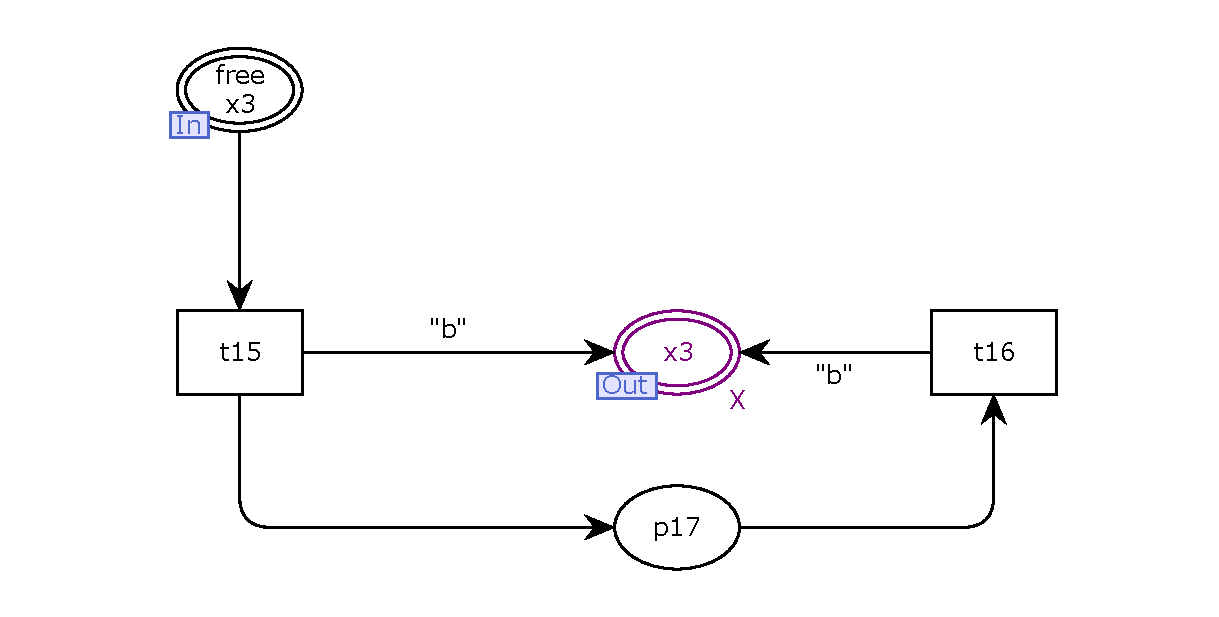
\includegraphics[width=0.6\linewidth]{figures//Simulation//Modelagem/controle_x3.eps}
    \legend{Fonte: Elaborado pelo autor.}
\end{figure}

\begin{figure}[ht]
    \centering
    \caption{Rede referente ao controle hierárquico X4 na RPC}
    \label{fig:controle_x4}
    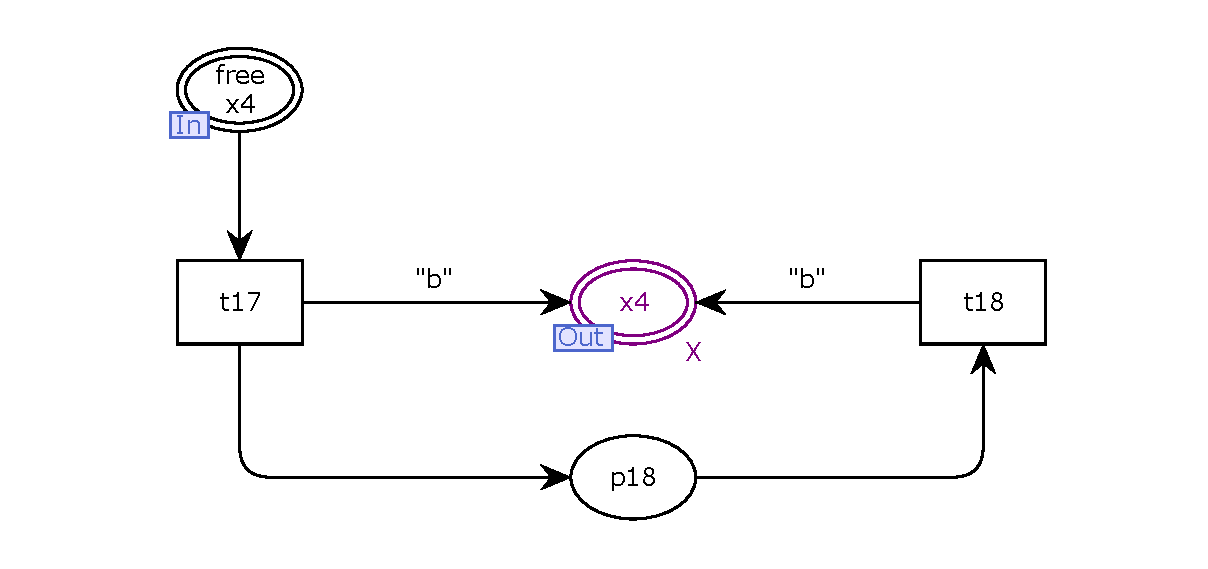
\includegraphics[width=0.6\linewidth]{figures//Simulation//Modelagem/controle_x4.eps}
    \legend{Fonte: Elaborado pelo autor.}
\end{figure}

\clearpage 
\subsubsection{Modelagem Ordenação dos vagões}
\label{sub:model_ord}
Na hierarquia trabalhada referente a figura \ref{fig:hierarquia_RPC}, que do modelo hierárquico referente a RPC, será demonstrado agora as redes relacionadas aos comando de coordenação dos vagões. Na camada de cima da hierarquia da pista as transições e lugares de ordem e inversão de ordem possuem comunicação principal com os controladores, como demonstrado na máscara do primeiro nível hierárquico na figura \ref{fig:pista_ordem}. Note que as informações de ultrapassagem e não ultrapassagem tem comunicação contro os \textit{Controladores} $X1$ e $X2$ e quem gerencia o primeiro($1_{st}$) e segundo($2_{nd}$) lugar são os dois componentes de \textit{Ordem} e\textit{ Inversão de Ordem}.

\begin{figure}[ht]
    \centering
    \caption{Máscara de componentes relacionados a ordem na RPC}
    \label{fig:pista_ordem}
    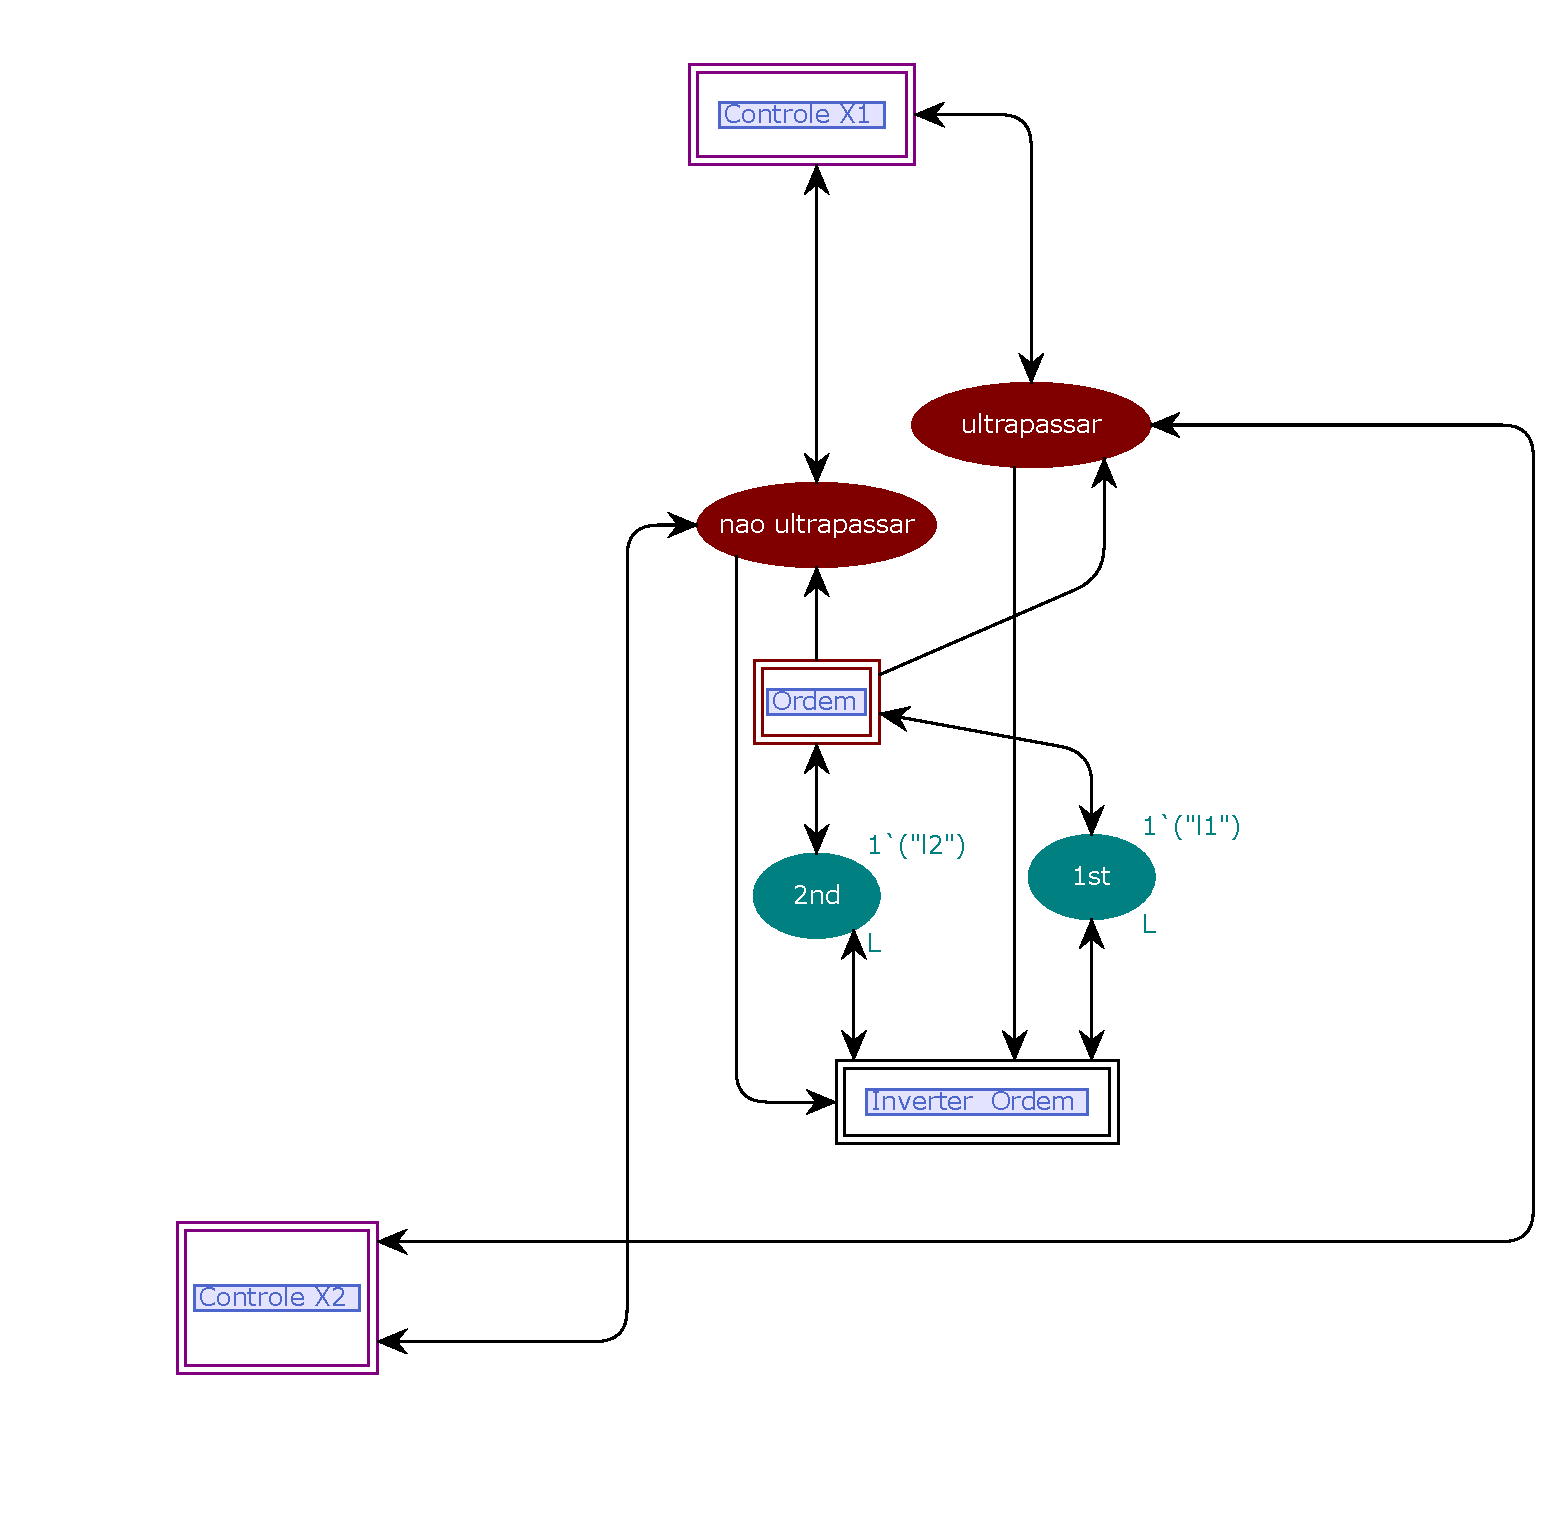
\includegraphics[width=0.8\linewidth]{figures//Simulation//Modelagem/pista_ordem.eps}
    \legend{Fonte: Elaborado pelo autor.}
\end{figure}

A transição hierárquica do componente de \textit{Ordem} é definida através da RPC demonstrada na figura \ref{fig:ordem}, para melhor compreensão a mesma foi dividade em duas máscaras uma de geração de comando e outra de restabelecimento da rede para geração de um novo comando.

\begin{figure}[ht]
    \centering
    \caption{Rede referente ao componente de Ordem na RPC}
    \label{fig:ordem}
    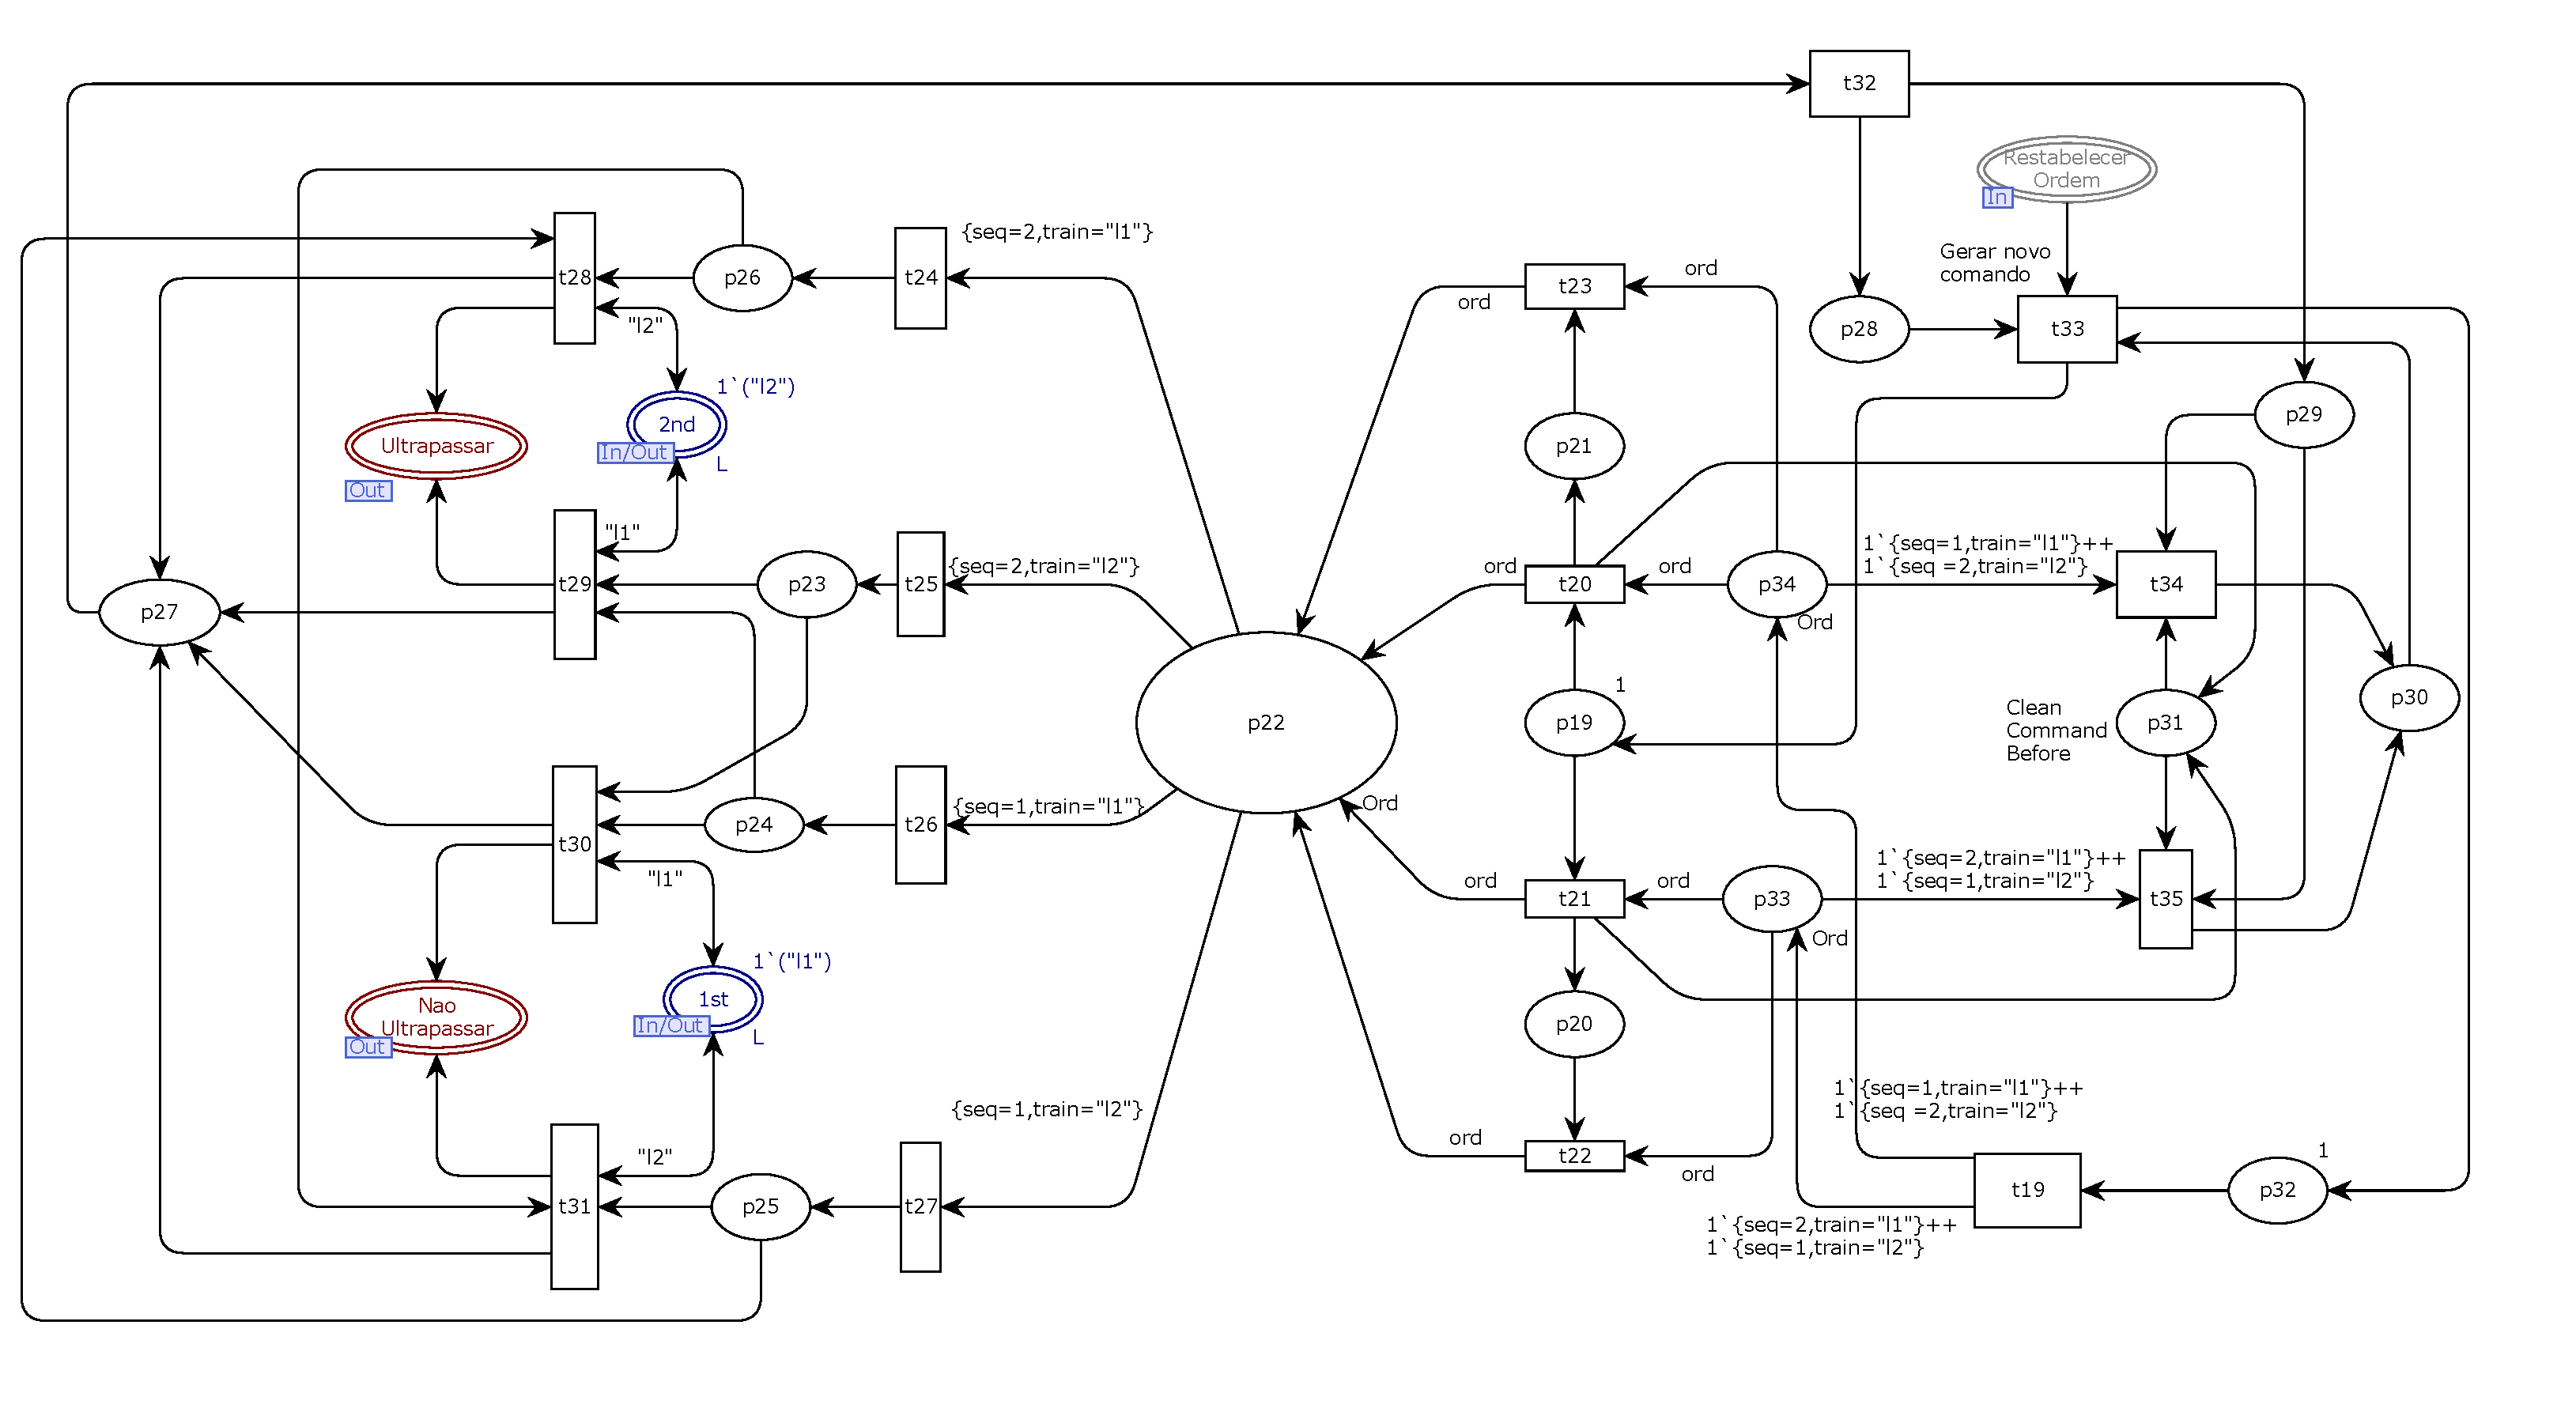
\includegraphics[width=1\linewidth]{figures//Simulation//Modelagem/ordem.eps}
    \legend{Fonte: Elaborado pelo autor.}
\end{figure}

Na geração do comando referente a ultrapassagem ou não ultrapassagem a parte da rede responsável é demonstrada na figura \ref{fig:geracao_ordem}, tal que no início da rede na transição $t_{19}$, são carregados dois comandos o primeiro comando que é recebido pelo lugar $p_{34}$ é o par da do vagão $l_1$ na posição 1 e o vagão $l_2$ na posição 2, através das fichas $1`\{seq=1,train="l1"\} ++ 1`\{seq=2,train="l2"\}$. De modo análogo o segundo comando é recebido pelo lugar $p_{33}$ referente ao vagão $l_2$ na posição 1 e o vagão $l_1$ na posição 2, através das fichas $1`\{seq=2,train="l1"\} ++ 1`\{seq=1,train="l2"\}$
Depois que os lugares $p_{33}$ e $p_{34}$ recebem as fichas as duas transições $t_{20}$ e $t_{21}$ ficam habilitadas ao mesmo tempo, de modo que o acionamento de uma ou outra é feito de forma aleatória. Por fim é feita a verificação de qual vagão está em primeiro e em segundo lugar pelos lugares $1_{st}$ e $2_{nd}$, respectivamente, para a partir disso ser gerado o comando de \textit{Ultrapassar} ou \textit{Não Ultrapassar}.

\begin{figure}[ht]
    \centering
    \caption{Máscara referente a geração de comando do componente de Ordem na RPC}
    \label{fig:geracao_ordem}
    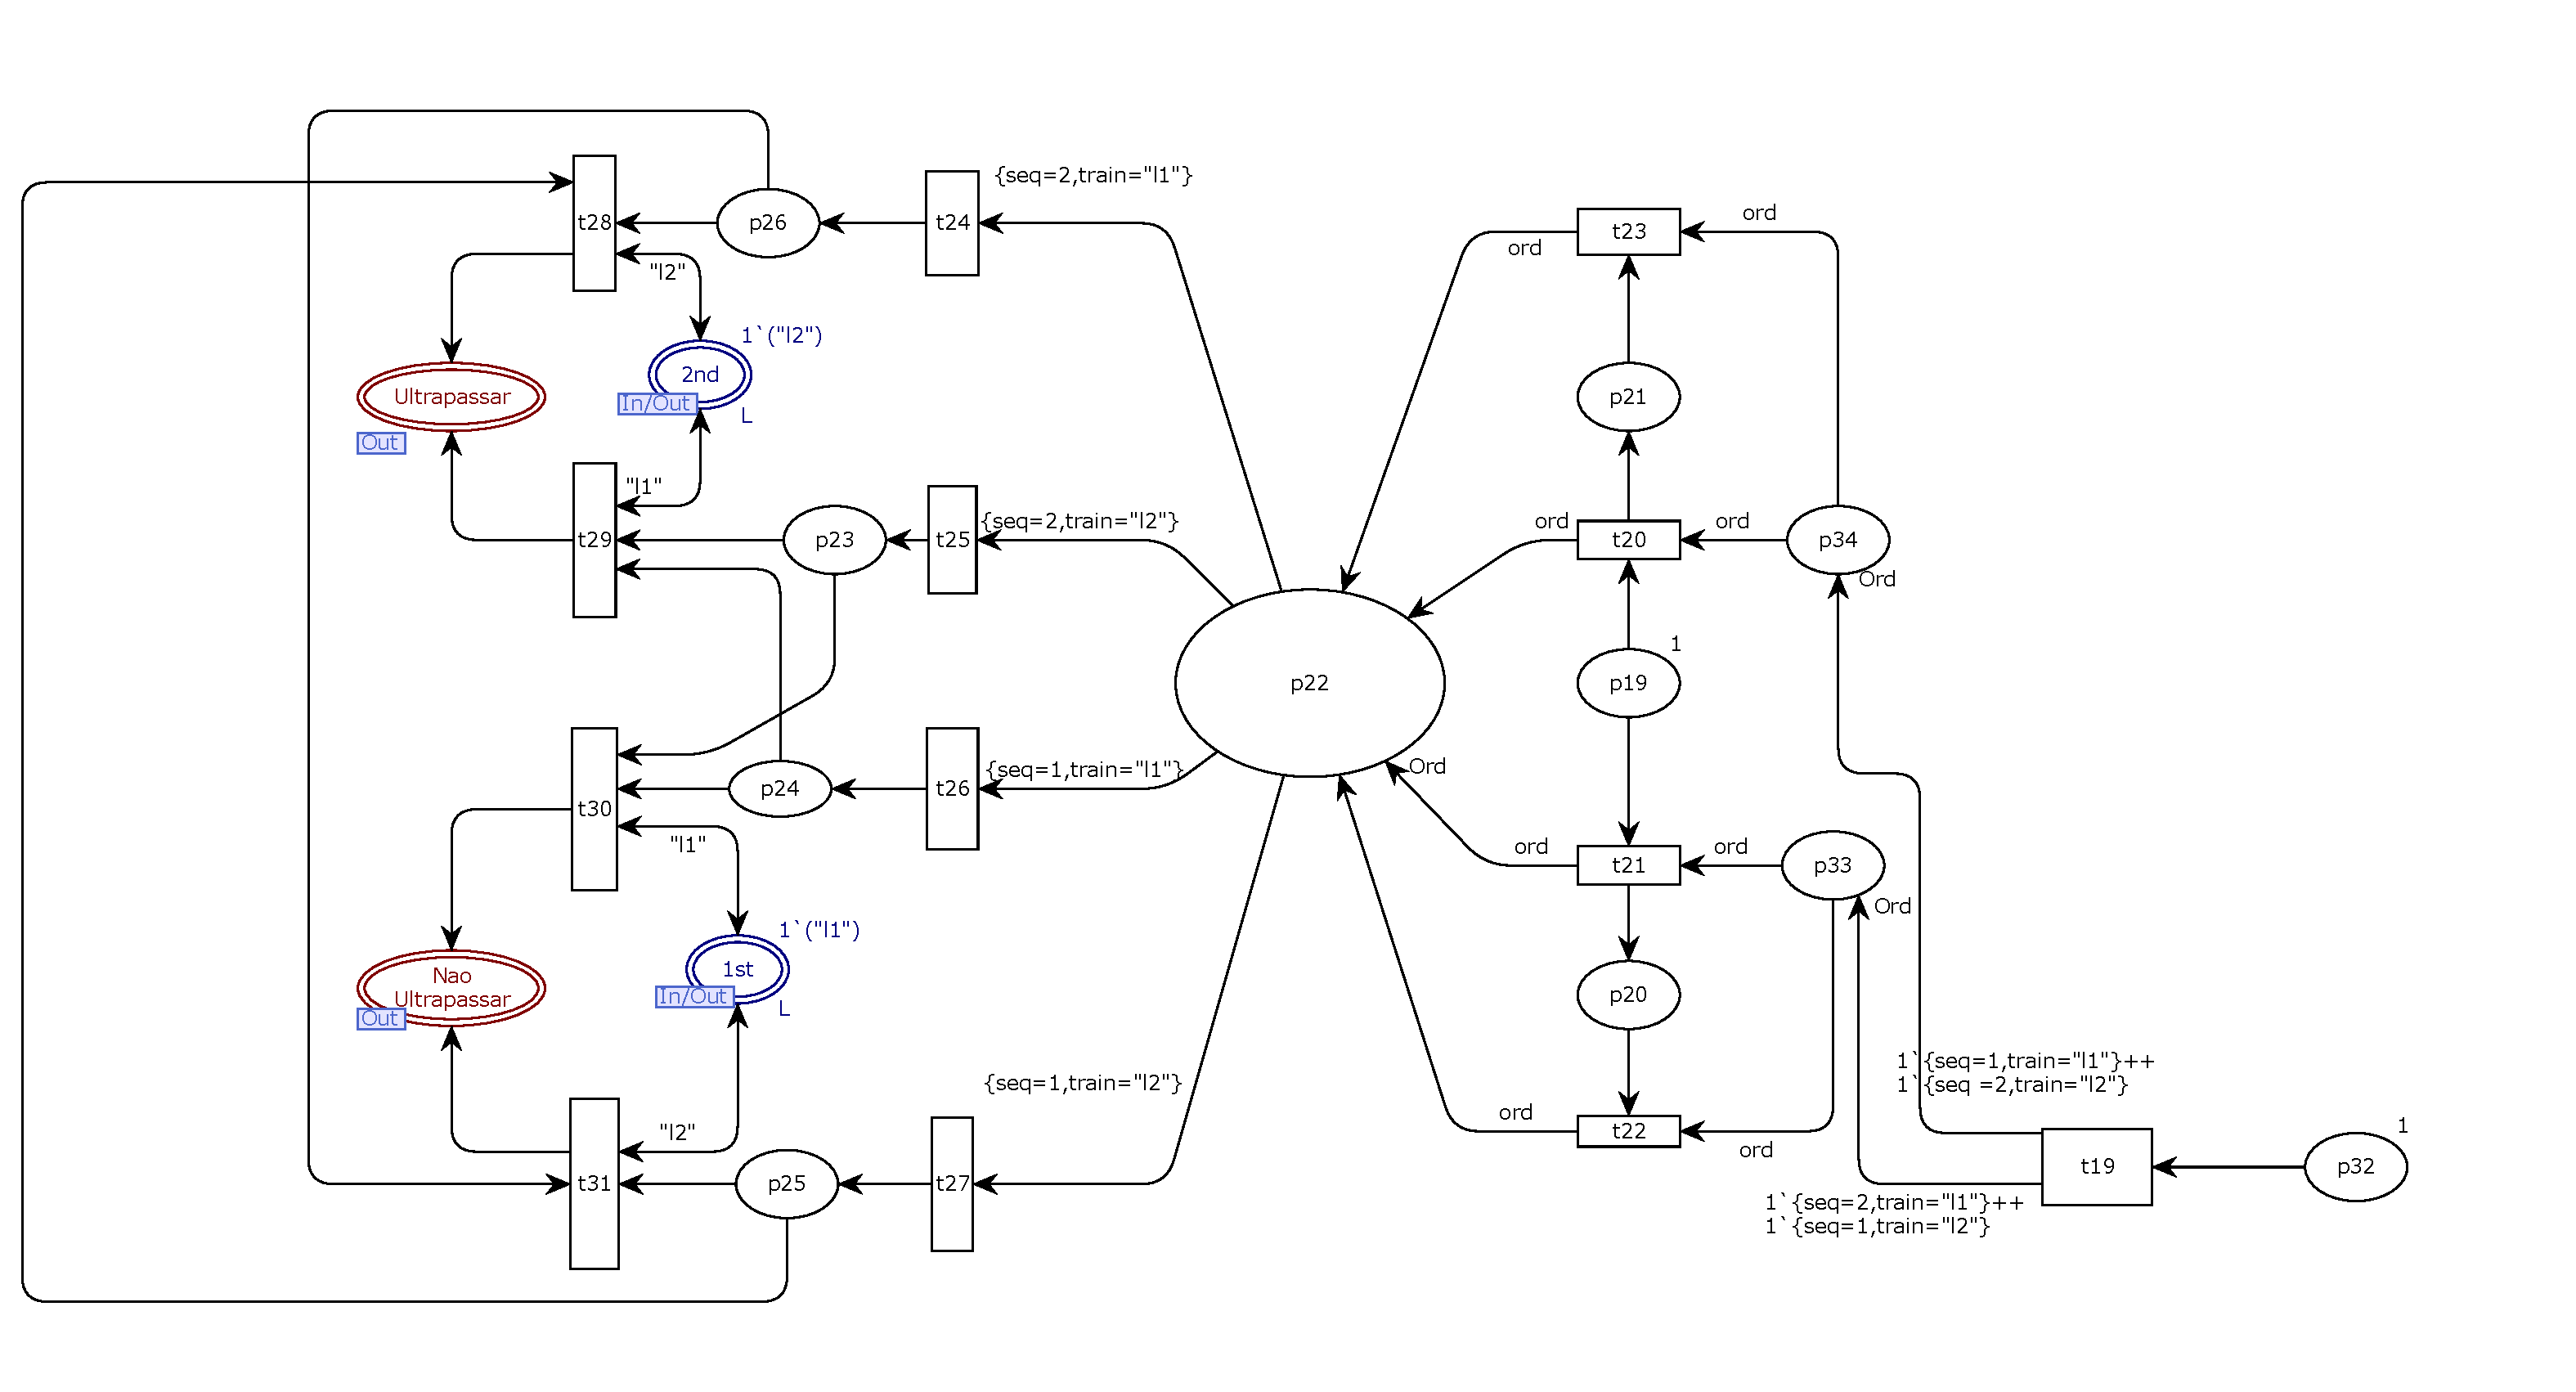
\includegraphics[width=1\linewidth]{figures/Simulation/Modelagem/geracao_ordem.eps}
    \legend{Fonte: Elaborado pelo autor.}
\end{figure}

Após gerado o comando de \textit{Ultrapassar} ou \textit{Não Ultrapassar} é necessário modelar o reestabelecimento da rede para que possa ser gerado novamente os comandos e não haja travamento da rede. O reestabelecimento é demonstrado na figura \ref{fig:restabelecer_ordem}, tal que após gerado os comandos que podem vir de qualquer uma das quatro transições $t_{28}, t_{29}, t_{30}, t_{31}$ a transição $t_32$ transfere uma ficha para $p_{28}$ que ativará a transição $t_{33}$ no momento de reestabelecer a ordem e uma ficha para o $p_{29}$ responsável por retirar a ficha que não foi utilizada durante a escolha aleatória de ordem.

\begin{figure}[ht]
    \centering
    \caption{Máscara referente ao restabelecimento do componente de Ordem na RPC}
    \label{fig:restabelecer_ordem}
    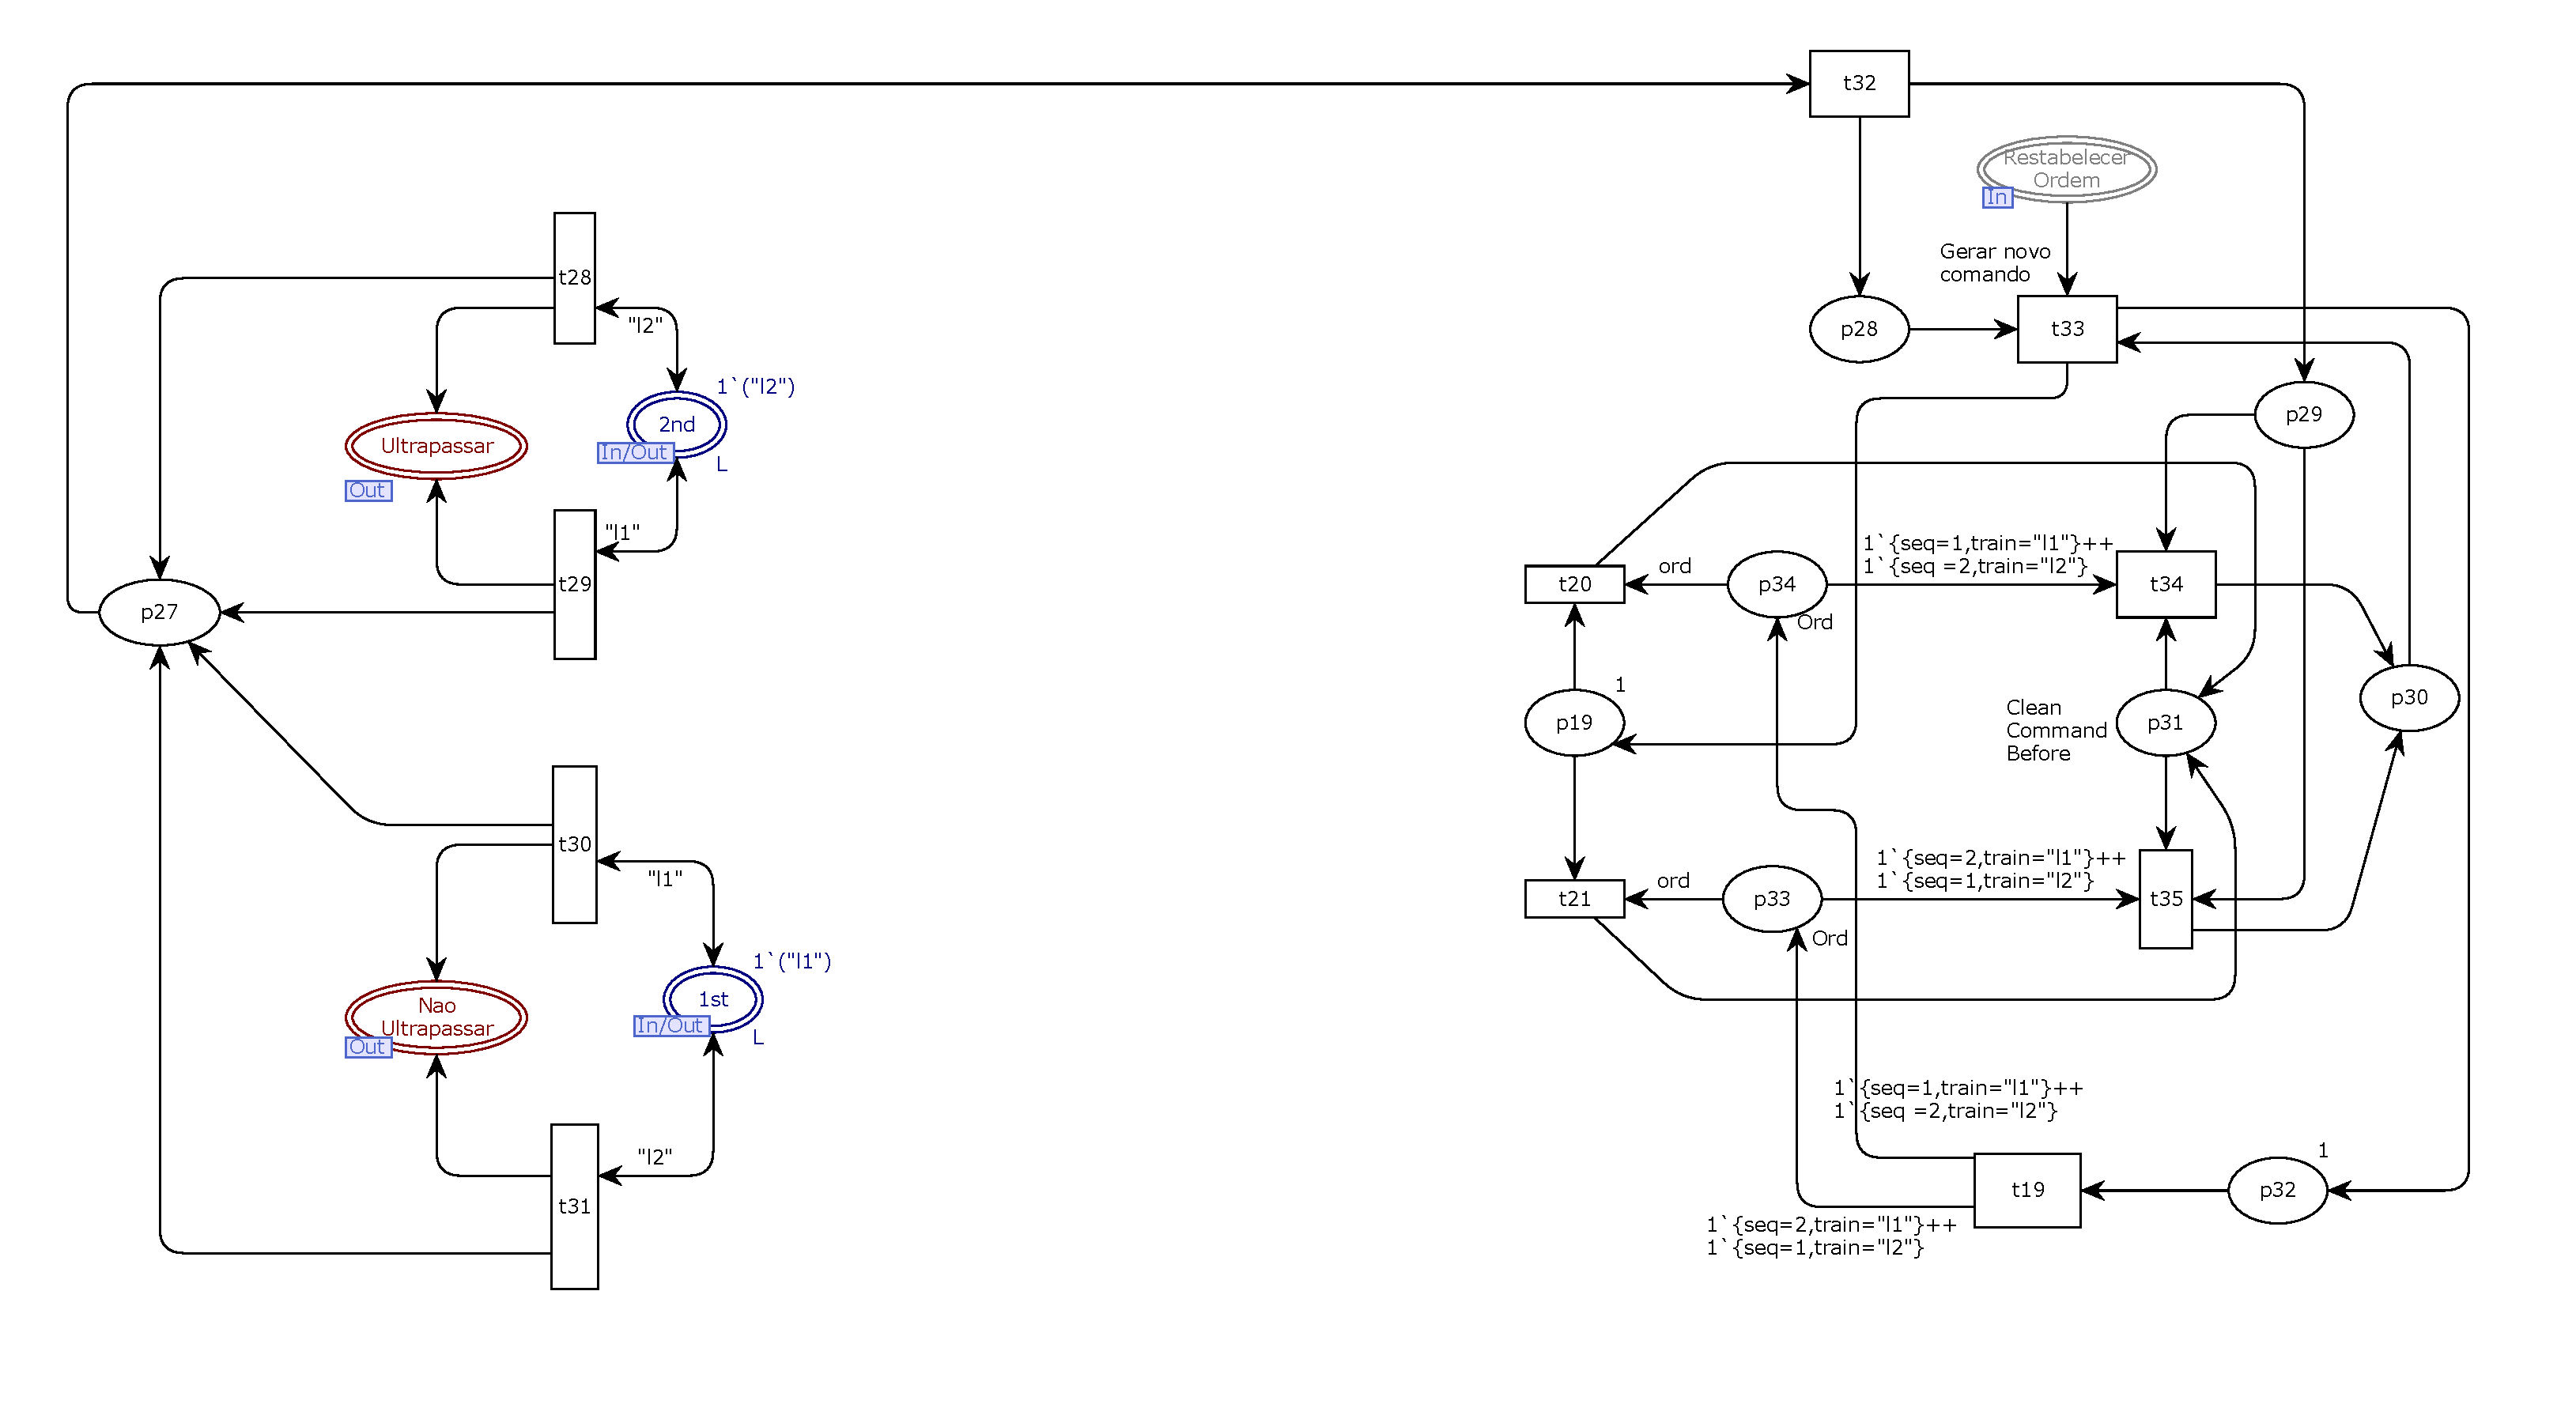
\includegraphics[width=1\linewidth]{figures/Simulation/Modelagem/restabelecer_ordem.eps}
    \legend{Fonte: Elaborado pelo autor.}
\end{figure}

O ultimo componente hierárquico da rede é o de \textit{Inverter Ordem}, responsável por atualizar os lugares de $1_{st}$ e $2_{nd}$, dado pela RPC representada na figura \ref{fig:inverter_ordem}. Note que ao chegar o comando de atualizar ordem caso haja uma ficha em ultrapassar, é ativado a transição $t_{36}$ que tem como objetivo retirar a ficha que estava em $2_{nd}$ guardar temporariamente em $p_{37}$ enquanto a ficha que estava em primeiro lugar é transferida para o segundo lugar e por fim é atualizado o primeiro lugar.
Caso não tenha ocorrido ultrapassagem a transição $t_{37}$ é acionada enviando o comando de \textit{Restabelecer a Rede} para a hierarquia a cima.

\begin{figure}[ht]
    \centering
    \caption{Máscara referente ao restabelecimento do componente de Ordem na RPC}
    \label{fig:inverter_ordem}
    \includegraphics[width=1\linewidth]{figures/Simulation/Modelagem/inverter_ordem.eps}
    \legend{Fonte: Elaborado pelo autor.}
\end{figure}

\subsection{Controle Cooperativo aplicado a Multiagentes}
Posteriormente à detalhada modelagem do sistema na seção \ref{sec:model_RPC} que foi definida os principais eventos do sistema, além da arquitetura da rede que gera algumas regras para o deslocamento dos vagões é buscada um controle de nível superior responsável por otimizar a referência de posição de cada vagão. Para o desenvolvimento do controle cooperativo entre os vagões com o objetivo de evitar   colisões e promover a otimização das trajetórias é importante garantir que as transições na rede de petri possuem acionamentos praticamente instantâneos não influenciando assim de forma significativa na dinâmica do sistema.

Para a coordenação e intercomunicação entre os agentes e a referência (agente virtual ou líder), foi escolhido o modelado o seguinte grafo \ref{fig:grafo_cooperativo}. Tal que $x_1$ e $x_2$, são os dois agentes da planta e o líder e dado por $x_3$. Note, que o grafo é classificado com um \textit{direct tree}, pois existe somente um líder o qual possui grau de entrada nulo, como apresentado na subseção \ref{sub:consenso_lider}. 

\begin{figure}[ht]
    \centering
    \caption{Modelagem do grafo entre agentes}
    \label{fig:grafo_cooperativo}
    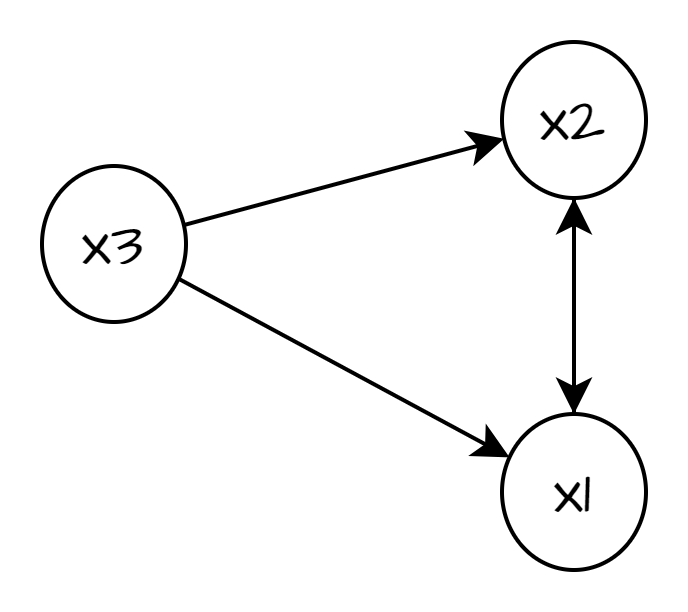
\includegraphics[width=0.4\linewidth]{figures/Simulation/Cooperativo/grafo_cooperativo.png}
    \legend{Fonte: Elaborado pelo autor.}
\end{figure}

Foram formulados dois tipos de problemática para o controle, o primeiro relacionado aos momentos que acontecem uma situação de ultrapassagem no ciclo de uma volta partindo e chagando em $d_1$ na pista da figura \ref{fig:pista_com_dois_agentes}, e o segundo o ciclo de uma volta sem ultrapassagem.

\subsubsection{Casos de Ultrapassagem}
Para a simulação e comportamento do controle por consenso nos casos de ultrapassagem foram escolhidas 4 referências diferentes para demonstrar o comportamento do sistema de acordo com a tabela \ref{tab:caso1_utrapassagem}. 
\begin{table}[ht]
    \centering
    \begin{tabular}{c|c}                 
         referência & trajetória  \\ \cline{1-2}
          0.5 & $d_1$ para $d_6$ e $d_3$  \\ \cline{1-2}
         -0.5 & $d_3$ e $d_6$ para $d_2$ \\ \cline{1-2}
         -0.2 & $d_2$ para $d_5$  \\ \cline{1-2}
            0 & $d_5$ para $d_1$ \\     
    \end{tabular}
    \caption{Escolha de referências ao longo do tempo com inversão de sinal}
    \label{tab:caso1_utrapassagem}
\end{table}

Para  primeira parte do algoritmo de controle cooperativo os valores dos pesos entre agentes, onde o agente \( R \) é considerado como a referência. Posteriormente, define-se a matriz de adjacência \( A \) e a matriz diagonal tal que \( A^T[0] \) corresponde à primeira linha de \( A \) transposta, \( A^T[1] \) à segunda linha e assim por diante, como demonstrado a seguir:
\[
A = \begin{bmatrix}
0 & a_{12} & 0 \\
a_{21} & 0 & 0 \\
a_{31} & a_{32} & 0
\end{bmatrix} ,
D = \begin{bmatrix}
sum(A^{T}[0]) & 0 & 0 \\
0 & sum(A^{T}[1]) & 0 \\
0 & 0 & sum(A^{T}[2])
\end{bmatrix}
\]
Para a construção da matriz Laplaciana, o valor final da matriz é determinado de acordo com a Equação \ref{eq:matriz_L1}, resultando no seguinte valor de L.
\[
L = \begin{bmatrix}
    sum(A^{T}[0]) & -a_{12} & 0 \\
    -a_{21} & sum(A^{T}[1]) & 0 \\
    -a_{31} & -a_{32} & sum(A^{T}[2])
    \end{bmatrix}
\]
Por fim o sistema resultante em espaço de estados é dado pelos seguintes valores de $A$, $B$, $C$ e $D$;
\[
A = -L 
 , 
 B = \begin{bmatrix}
    1\\
    0\\
    0\\
\end{bmatrix}
 ,
C = \begin{bmatrix}
    1 & 0 & 0\\
    0 & 1 & 0\\
    0 & 0 & 1\\
\end{bmatrix}
 ,
D = 0
\]
Por meio da simulação com todos os pesos nos arcos iguais a $0.5$ é obtido a seguinte o gráfico da figura \ref{fig:case1}. Note que inicialmente é praticamente  considerado que os dois iniciam praticamente junto e vão se separando no tempo de 0 a 20 minutos, até que ao chegar aproximadamente em torno de 30 segundo a referência é alterada e é feita uma ultrapassagem nos momentos seguintes as colocações se mantêm mas a distância entre os agentes vai cada vez mais diminuindo coma escolha das referências. 

\begin{figure}[ht]
    \centering
    \caption{Simulação Caso de Ultrapassagem}
    \label{fig:case1}
    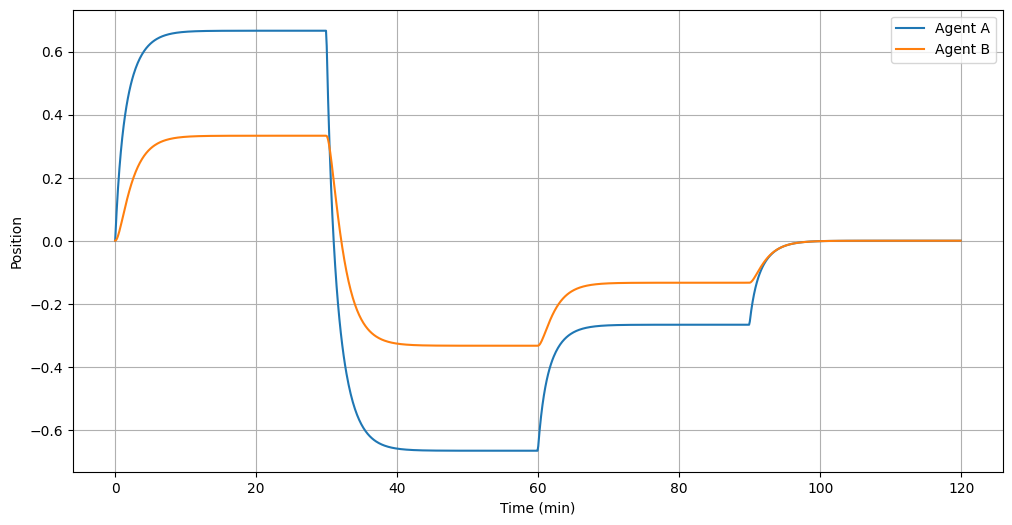
\includegraphics[width=1\linewidth]{figures/Simulation/Cooperativo/case1.png}
    \legend{Fonte: Elaborado pelo autor.}
\end{figure}

A partir da figura \ref{fig:case1_fig2} é visualizado o comportamento da velocidade entre os agentes assim como as mudanças de referência, note que mesmo o líder submetido a valores constantes de referência, o sistema gradualmente estabiliza naquele ponto de referência, gerando assim uma mudança de referência mais suave.
\begin{figure}[ht]
    \centering
    \caption{Análise velocidade Caso de Ultrapassagem}
    \label{fig:case1_fig2}
    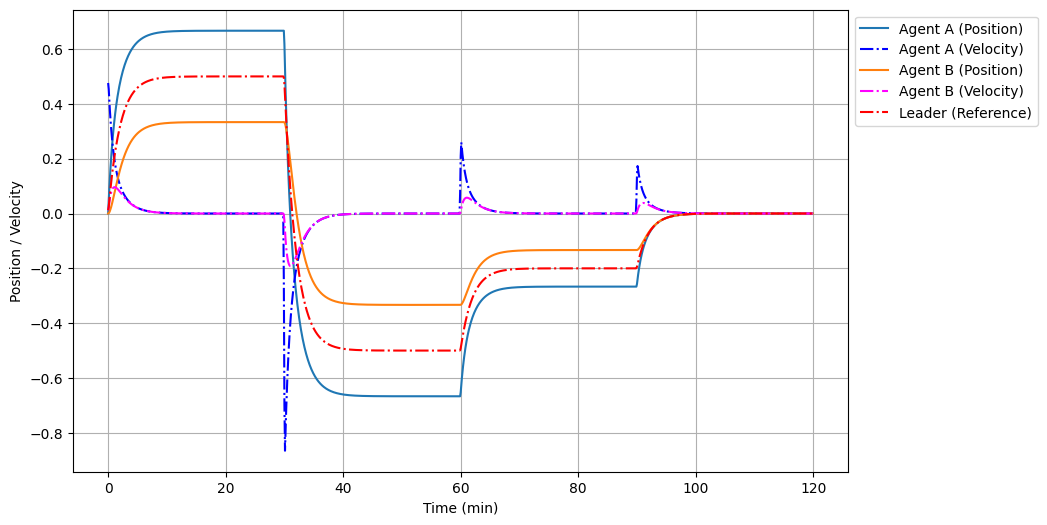
\includegraphics[width=1\linewidth]{figures/Simulation/Cooperativo/case1_fg2.png}
    \legend{Fonte: Elaborado pelo autor.}
\end{figure}

Um segundo resultado é obtido diminuindo a em torno de 4x a comunicação com o líder, mas mantendo o mesmo valor de comunicação entre os agentes. Tal exemplo é demonstrada na figura \ref{fig:case2_fig2}, note que para esse caso a formação dos agentes se mantém ao longo de todas as mudanças de referência, o que muda é a velocidade em que os agentes alcançam a velocidade relativa de zero. Na aplicação proposta esse comportamento não é desencorajado uma vez que o foco tem sido o mantimento da formação nos casos de ultrapassagem.

\begin{figure}[ht]
    \centering
    \caption{Análise Diminuição do peso da comunicação com o líder no Caso de Ultrapassagem}
    \label{fig:case2_fig2}
    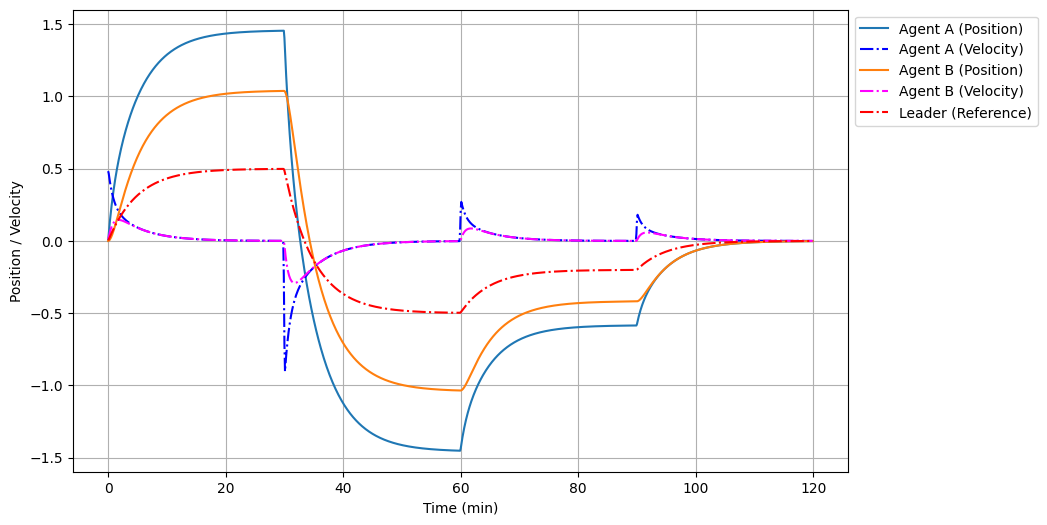
\includegraphics[width=1\linewidth]{figures/Simulation/Cooperativo/case2_fg2.png}
    \legend{Fonte: Elaborado pelo autor.}
\end{figure}

Ainda na análise com os valores de referência descritos na tabela \ref{tab:caso1_utrapassagem}, um importante ponto a ser realçado é que para manter a mesma configuração com a ultrapassagem somente no ponto onde a referência é dada como negativa é importante que o peso dos arcos entre os agentes seja semelhantes, pois a medida que a diferença aumenta  a velocidade em que um agente procura a referência é maior que a do outro, podendo ocasionar uma segunda ultrapassagem, exemplo desse comportamento evitado para a aplicação dada é demonstrado na figura \ref{fig:case3_fig2}. Note que o perfil de velocidade se assemelha nos dois casos, mas na posição é possível perceber que em torno de 90 min o agente A vai de encontro a referência do líder mais rapidamente que o Agente B, ocasionando uma segunda ultrapassage, e de fato para essa simulação o peso do arco do agente A em relação com o líder em relação ao agente B com o líder é em torno de 4x maior.

\begin{figure}[ht]
    \centering
    \caption{Análise pesos muito diferentes na comunicação com o líder Caso de Ultrapassagem}
    \label{fig:case3_fig2}
    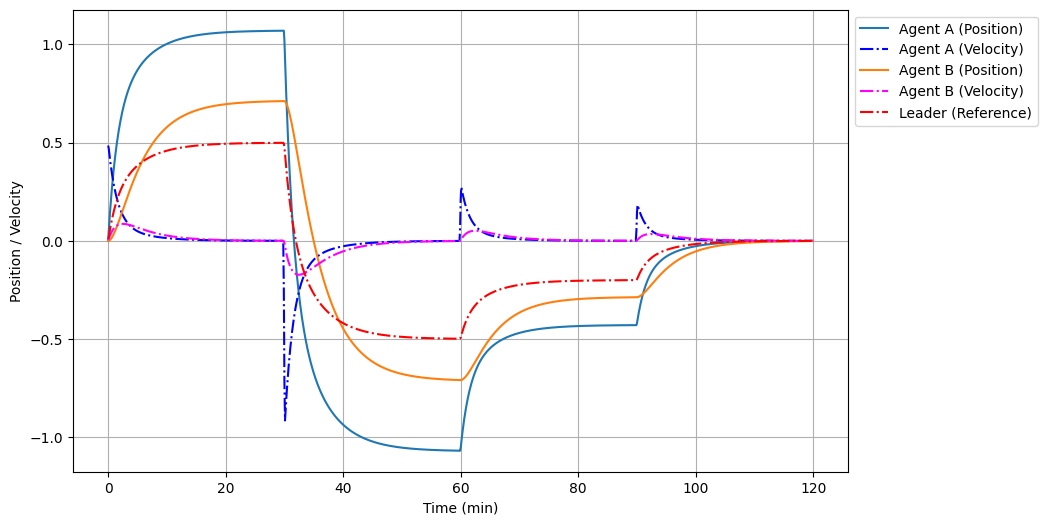
\includegraphics[width=1\linewidth]{figures/Simulation/Cooperativo/case3_fg2.png}
    \legend{Fonte: Elaborado pelo autor.}
\end{figure}

\subsubsection{Casos de Não Ultrapassagem}
O segundo grupo de simulações é relacionado aos casos onde não é necessário que ocorra ultrapassagem entre os agentes, ou seja a formação inicial seja mantida ao longo das mudanças de referência. Para isso é utilizado os valores de referência de acordo com a a tabela \ref{tab:caso1_sem_utrapassagem}
\begin{table}[ht]
    \centering
    \begin{tabular}{c|c}                 
         referência & trajetória  \\ \cline{1-2}
         0.2 & $d_1$ para $d_6$ e $d_3$  \\ \cline{1-2}
         0.5 & $d_3$ e $d_6$ para $d_2$ \\ \cline{1-2}
         0.2 & $d_2$ para $d_5$  \\ \cline{1-2}
            0 & $d_5$ para $d_1$ \\     
    \end{tabular}
    \caption{Escolha de referências ao longo do tempo sem inversão de sinal}
    \label{tab:caso1_sem_utrapassagem}
\end{table}

Por meio da simulação com todos os pesos nos arcos iguais a $0.5$ é obtido a seguinte o gráfico da figura \ref{fig:case4}. Note que inicialmente é considerado que os dois iniciam praticamente junto e vão se separando no tempo de 0 a 20 minutos, e em quanto o valor de referência sobe, a distância entre eles aumenta até o momento que a referência começa a diminuir. Note que a formação do grupo de agentes se mantém a mesma ao longo de diferentes valores de referência positiva.

\begin{figure}[ht]
    \centering
    \caption{Simulação Caso de não ultrapassagem}
    \label{fig:case4}
    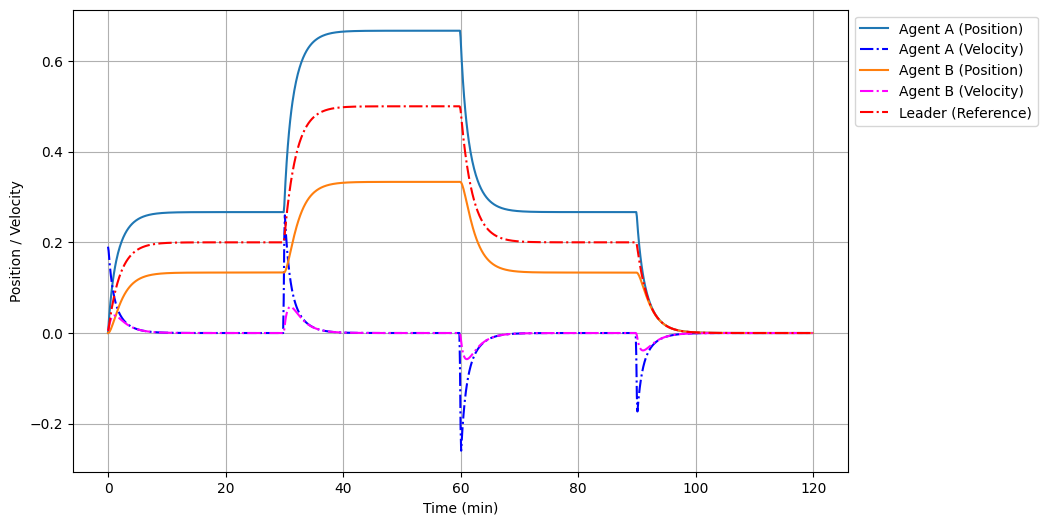
\includegraphics[width=1\linewidth]{figures/Simulation/Cooperativo/case4_fg2.png}
    \legend{Fonte: Elaborado pelo autor.}
\end{figure}

De forma análoga um segundo resultado é obtido diminuindo em torno de 4x a comunicação com o líder, mas mantendo o mesmo valor de comunicação entre os agentes. Tal exemplo é demonstrada na figura \ref{fig:case5}, note que para esse caso a formação dos agentes se mantém ao longo de todas as mudanças de referência, o que muda é a velocidade em que os agentes alcançam a velocidade relativa de zero.

\begin{figure}[ht]
    \centering
    \caption{Simulação Caso de não ultrapassagem, diminuição peso comunicação com o líder}
    \label{fig:case5}
    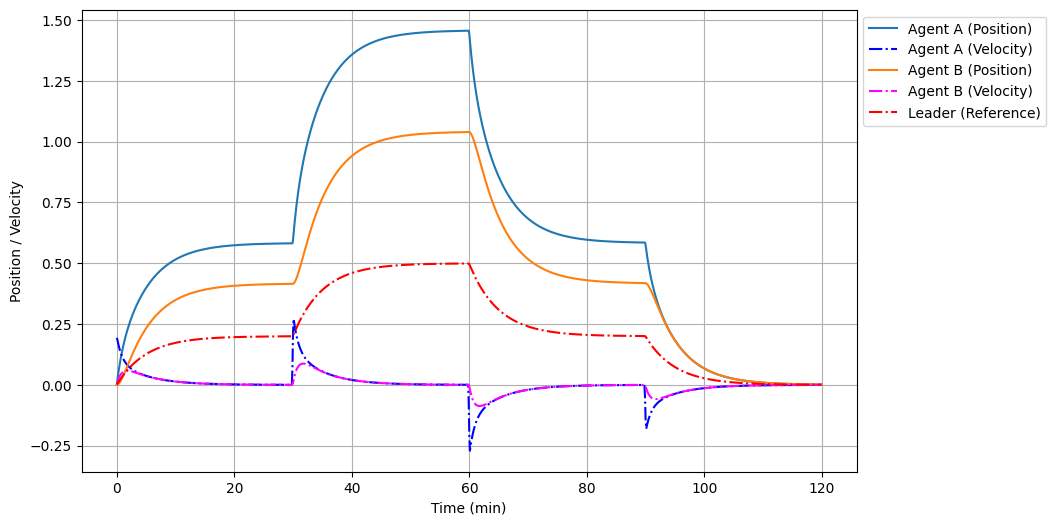
\includegraphics[width=1\linewidth]{figures/Simulation/Cooperativo/case5_fg2.png}
    \legend{Fonte: Elaborado pelo autor.}
\end{figure}

Por fim, para fins de análise, é refeito o testes de pesos desbalanceados em relação ao líder, o resultado é demonstrado na figura \ref{fig:case6}, note que o mesmo tipo de comportamento acontece como demonstrado no caso de ultrapassagem, em que a formação é alterada perto do ponto de referência nula do líder. No caso de manter a formação tal comportamento não é desejado.
\begin{figure}[ht]
    \centering
    \caption{Simulação Caso de não ultrapassagem, grande diferença peso na comunicação com o líder}
    \label{fig:case6}
    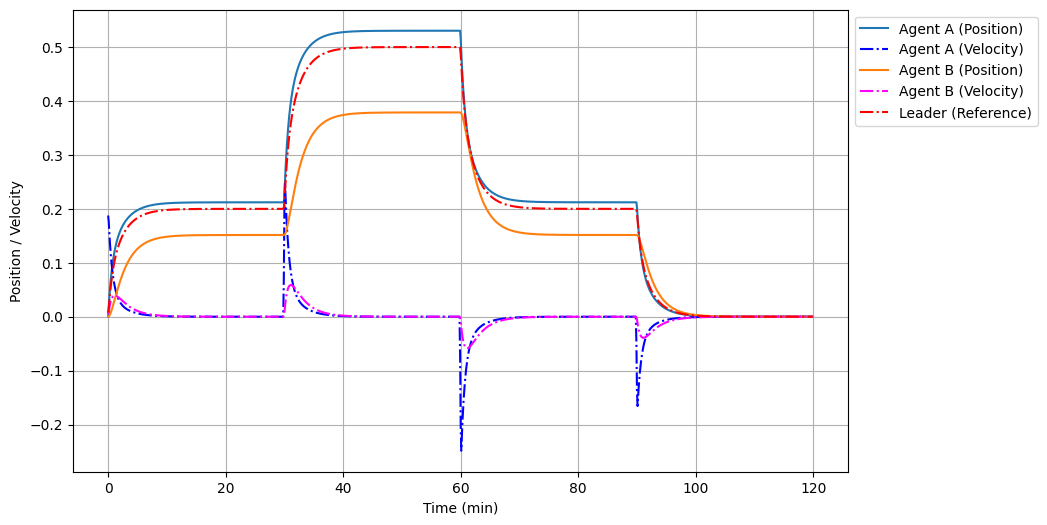
\includegraphics[width=1\linewidth]{figures/Simulation/Cooperativo/case6_fg2.png}
    \legend{Fonte: Elaborado pelo autor.}
\end{figure}
